%======================================================================
% Based on: University of Waterloo Thesis Template for LaTeX 
%======================================================================

% DON'T FORGET TO ADD YOUR OWN NAME AND TITLE in the "hyperref" package configuration below. 
% THIS INFORMATION GETS EMBEDDED IN THE PDF FINAL PDF DOCUMENT.
% You can view the information if you view properties of the PDF document.

% Contains options for print optimization, which I have commented out.

% Compile
% E.g. to process a thesis called "mythesis.tex" based on this template, run:

% pdflatex mythesis	-- first pass of the pdflatex processor
% bibtex mythesis	-- generates bibliography from .bib data file(s)
% makeindex         -- should be run only if an index is used 
% pdflatex mythesis	-- fixes numbering in cross-references, bibliographic references, glossaries, index, etc.
% pdflatex mythesis	-- it takes a couple of passes to completely process all cross-references

% N.B. The "pdftex" program allows graphics in the following formats to be included with the "\includegraphics" command: PNG, PDF, JPEG, TIFF
% Tip: Generate your figures and photos in the size you want them to appear in your thesis, rather than scaling them with \includegraphics options.
% Tip: Any drawings you do should be in scalable vector graphic formats: SVG, PNG, WMF, EPS and then converted to PNG or PDF, so they are scalable in the final PDF as well.
% Tip: Photographs should be cropped and compressed so as not to be too large.

% To create a PDF output that is optimized for double-sided printing: 
% 1) comment-out the \documentclass statement in the preamble below, and un-comment the second \documentclass line.
% 2) change the value assigned below to the boolean variable "PrintVersion" from " false" to "true".

%======================================================================
%   D O C U M E N T   P R E A M B L E
% Specify the document class, default style attributes, and page dimensions, etc.
% For hyperlinked PDF, suitable for viewing on a computer, use this:
\documentclass[letterpaper,12pt,titlepage,oneside,final]{book}
 
% For PDF, suitable for double-sided printing, change the PrintVersion variable below to "true" and use this \documentclass line instead of the one above:
%\documentclass[letterpaper,12pt,titlepage,openright,twoside,final]{book}

% Some LaTeX commands I define for my own nomenclature (template
\newcommand{\cmmd}[1]{\textbackslash\texttt{#1}} % command name in tt font 
\newcommand{\href}[1]{#1} % does nothing, but defines the command so the print-optimized version will ignore \href tags (redefined by hyperref pkg).

%% PACKAGES %%

% This package allows if-then-else control structures.
\usepackage{ifthen}
\newboolean{PrintVersion}
\setboolean{PrintVersion}{false}
% CHANGE THIS VALUE TO "true" as necessary, to improve printed results for hard copies by overriding some options of the hyperref package, called below.

\usepackage{amsmath,amssymb,amstext} % Lots of math symbols and environments
\usepackage[pdftex]{graphicx} % For including graphics N.B. pdftex graphics driver 
\usepackage{siunitx}
\usepackage{caption}
\usepackage{subcaption}
\usepackage{xcolor}
\usepackage{tabularx}
\usepackage{scalerel}
\usepackage{geometry}

% My latex commands
\newcommand{\package}[1]{\texttt{#1}} % package names in bold text
\def\msquare{\mathord{\scalerel*{\Box}{gX}}} % to make a "square" shape in math mode

% Hyperlinks make it very easy to navigate an electronic document.
% In addition, this is where you should specify the thesis title and author as they appear in the properties of the PDF document.
% Use the "hyperref" package 
% N.B. HYPERREF MUST BE THE LAST PACKAGE LOADED; ADD ADDITIONAL PKGS ABOVE
\usepackage[pdftex,pagebackref=false]{hyperref} % with basic options
%\usepackage[pdftex,pagebackref=true]{hyperref}
		% N.B. pagebackref=true provides links back from the References to the body text. This can cause trouble for printing.
\hypersetup{
    plainpages=false,       % needed if Roman numbers in frontpages
    unicode=false,          % non-Latin characters in Acrobat’s bookmarks
    pdftoolbar=true,        % show Acrobat’s toolbar?
    pdfmenubar=true,        % show Acrobat’s menu?
    pdffitwindow=false,     % window fit to page when opened
    pdfstartview={FitH},    % fits the width of the page to the window
    pdftitle={Using cosmic-ray hodoscope data to validate the misalignment model of small-strip thin gap chambers for the ATLAS new small wheels},
    pdfauthor={Lia Formenti},
    pdfsubject={Using cosmic-ray hodoscope data to validate the misalignment model of small-strip thin gap chambers for the ATLAS new small wheels},
%    pdfkeywords={keyword1} {key2} {key3}, % list of keywords, and uncomment this line if desired
    pdfnewwindow=true,      % links in new window
    colorlinks=true,        % false: boxed links; true: colored links
    linkcolor=blue,         % color of internal links
    citecolor=green,        % color of links to bibliography
    filecolor=magenta,      % color of file links
    urlcolor=cyan           % color of external links
}
\ifthenelse{\boolean{PrintVersion}}{   % for improved print quality, change some hyperref options
\hypersetup{	% override some previously defined hyperref options
%    colorlinks,%
    citecolor=black,%
    filecolor=black,%
    linkcolor=black,%
    urlcolor=black}
}{} % end of ifthenelse (no else)

\usepackage[automake,toc,abbreviations]{}
% \usepackage[automake,toc,abbreviations]{glossaries-extra} % Exception to the rule of hyperref being the last add-on package
% If glossaries-extra is not in your LaTeX distribution, get it from CTAN (http://ctan.org/pkg/glossaries-extra), 
% although it's supposed to be in both the TeX Live and MikTeX distributions. There are also documentation and 
% installation instructions there.

%% STYLE %%

% Setting up the page margins...
% uWaterloo thesis requirements specify a minimum of 1 inch (72pt) margin at the
% top, bottom, and outside page edges and a 1.125 in. (81pt) gutter margin (on binding side). 
% While this is not an issue for electronic viewing, a PDF may be printed, and so we have the same page layout for both printed and electronic versions, we leave the gutter margin in.
% Set margins to minimum permitted by uWaterloo thesis regulations:
\setlength{\marginparwidth}{0pt} % width of margin notes
% N.B. If margin notes are used, you must adjust \textwidth, \marginparwidth
% and \marginparsep so that the space left between the margin notes and page
% edge is less than 15 mm (0.6 in.)
% \setlength{\marginparsep}{0.125pt} % width of space between body text and margin notes
% Changed even/oddsidemargin from 0.125 to 0 because I think I will only make an electronic copy. Changed textwidth to match. - LF
\setlength{\evensidemargin}{0in} % Adds 1/8 in. to binding side of all 
% even-numbered pages when the "twoside" printing option is selected
\setlength{\oddsidemargin}{0in} % Adds 1/8 in. to the left of all pages when "oneside" printing is selected, and to the left of all odd-numbered pages when "twoside" printing is selected
\setlength{\textwidth}{6.5in} % assuming US letter paper (8.5 in. x 11 in.) and side margins as above
\raggedbottom

% The following statement specifies the amount of space between paragraphs. Other reasonable specifications are \bigskipamount and \smallskipamount.
\setlength{\parskip}{\medskipamount}

% The following statement controls the line spacing.  
% The default spacing corresponds to good typographic conventions and only slight changes (e.g., perhaps "1.2"), if any, should be made.
\renewcommand{\baselinestretch}{1} % this is the default line space setting

% Remove paragraph indentation
\setlength{\parindent}{0pt}

% Commented out because you aren't printing and this is a waste of paper - LF
% By default, each chapter will start on a recto (right-hand side) page.
% We also force each section of the front pages to start on a recto page by inserting \cleardoublepage commands.
% In many cases, this will require that the verso (left-hand) page be blank, and while it should be counted, a page number should not be printed.
% The following statements ensure a page number is not printed on an otherwise blank verso page.
% \let\origdoublepage\cleardoublepage
% \newcommand{\clearemptydoublepage}{%
%  \clearpage{\pagestyle{empty}\origdoublepage}}
% \let\cleardoublepage\clearemptydoublepage

% Define Glossary terms (This is properly done here, in the preamble and could also be \input{} from a separate file...)
% \input{glossaries}
% \makeglossaries

% My commands
%\newcommand{\um}{$\upmu$m} % micrometers
%\newcommand{\urad}{$\upmu$rad} % microrads

%======================================================================
%   L O G I C A L    D O C U M E N T
% The logical document contains the main content of your thesis.
% Being a large document, it is a good idea to divide your thesis into several files, each one containing one chapter or other significant chunk of content, so you can easily shuffle things around later if desired.
%======================================================================
\begin{document}

%----------------------------------------------------------------------
% FRONT MATERIAL
% title page,declaration, borrowers' page, abstract, acknowledgements,
% dedication, table of contents, list of tables, list of figures, nomenclature, etc.
%----------------------------------------------------------------------
% T I T L E   P A G E
% -------------------
% Last updated October 23, 2020, by Stephen Carr, IST-Client Services
% The title page is counted as page `i' but we need to suppress the
% page number. Also, we don't want any headers or footers.
\pagestyle{empty}
\pagenumbering{roman}

% The contents of the title page are specified in the "titlepage"
% environment.
\begin{titlepage}
        \begin{center}
        \vspace*{1.0cm}

        \Huge
        {\bf Cosmic ray validation of electrode positions in small-strip thin gap chambers for the upgrade of the ATLAS detector } \\

        \vspace*{1.0cm}

        \Large
        Lia Formenti \\
        
        \vspace*{1.0cm}
        
        \normalsize
        Department of Physics \\
        McGill University, Montreal \\
        October, 2021 \\

        \vspace*{3.0cm}

        \normalsize
        A thesis submitted to\\
        McGill University \\ 
        in partial fulfillment of the \\
        requirements of the degree of \\
        Master of Science \\

        \vspace*{2.0cm}

        \copyright\ Lia Formenti 2021 \\
        \end{center}
\end{titlepage}

% The rest of the front pages should contain no headers and be numbered using Roman numerals starting with `ii'
\pagestyle{plain}
\setcounter{page}{2}

\cleardoublepage % Ends the current page and causes all figures and tables that have so far appeared in the input to be printed.
% In a two-sided printing style, it also makes the next page a right-hand (odd-numbered) page, producing a blank page if necessary.

% T A B L E   O F   C O N T E N T S
% ---------------------------------
\renewcommand\contentsname{Table of Contents}
\tableofcontents
\cleardoublepage
\phantomsection    % allows hyperref to link to the correct page

% A B S T R A C T
% ---------------

\begin{center}\textbf{Abstract}\end{center}
% Medium length abstract
% The particle collision rate at the Large Hadron Collider (LHC) will be effectively increased in 2025-2027 by an extensive upgrade program. The upgrades will improve the statistics on measurements and the sensitivity of searches for rare processes using the ATLAS experiment and other experiments at the LHC. The innermost endcaps of the ATLAS muon spectrometer consist of two wheels of muon detectors that must be replaced to maintain the muon momentum resolution in the high-rate environment. The so-called New Small Wheels (NSWs) are covered with two detector technologies: micromegas and small-strip thin gap chambers (sTGCs). Canada is responsible for 1/4 of the required sTGCs. sTGCs are gas ionization chambers that hold a thin volume of gas between two cathode boards. One board is segmented into strips of \SI{3.2}{mm} pitch that are used to precisely measure the coordinate of a passing muon. Four sTGCs glued together, called a quadruplet, cover the NSWs. Quadruplets were designed to achieve \SI{1}{mrad} angular resolution to fulfill the spectrometer's precision tracking and triggering requirements. A requirement to deliver the angular resolution is positioning the strips in the ATLAS coordinate system to within the chambers' position resolution (less than \SI{100}{\micro\meter}). The ATLAS alignment system is able to position the surface of the quadruplets, so the interal geometry of the quadruplets must be characterized. At McGill University, quadruplets are characterized using a cosmic ray hodoscope before being sent to CERN, where the charge profile left by x-rays is used to measure the local offset of the strip pattern at specific positions on the quadruplet surface. The x-ray method has acceptable but limited precision. It is being used to position the strips within the ATLAS alignment system. Given the importance of alignment, the x-ray method must be validated by an external method. Cosmic ray data is used to characterize the relative alignment between layers and validate the x-ray method.

% Too long version of abstract (rough)
% The collision rate in the LHC will be effectively increased in 2025-2027 by an extensive upgrade program. The innermost endcaps of the ATLAS muon spectrometer consist of two wheels of muon detectors that must be replaced to improve the angular resolution of tracks for precision muon momentum reconstruction. The New Small Wheels (NSWs) will be covered with two detector types that must trigger on and track outgoing particles: micromegas and small-strip thin gap chambers (sTGCs). Canada is responsible for one quarter of the required sTGCs.  sTGCs are gas ionization chambers that hold a thin volume of gas between two cathode boards. One board is segmented into strips of \SI{3.2}{mm} pitch that are used to measure the precision coordinate. At McGill University, modules with four layers of sTGCs called quadruplets are characterized using a cosmic ray hodoscope before being sent to CERN for further testing and integration into the wheels. Quadruplets must be able to reconstruct particle tracks with 1 mrad angular resolution using the precision coordinate recorded by the strips of each sTGC layer for ATLAS' physics goals. A requisite to delivering the angular resolution is positioning the strips in the ATLAS coordinate system to within the chambers' position resolution (\SI{100}{\micro\meter}). The ATLAS alignment system will be able to position alignment platforms on the surface of quadruplets, so the internal geometry of the chambers must be measured and corrected for. Analyzing the residuals of cosmic ray tracks is used to measure the offset of the strip pattern on one layer with respect to other layers in areas of interest. Looking at the relative offsets over the surface of an sTGC layer characterizes the quadruplets' relative alignment. To get the strip pattern offsets in ATLAS' absolute coordinate system, the charge profile left by an x-ray gun is used to measure the offset of the strip pattern from nominal. These offsets are used to create an alignment model for each sTGC strip layer. The x-ray measurements are limited to the positions of the alignment platform and have limited precision, so their accuracy must be verified by an independent method. In this work, cosmic ray data is used to study the relative alignment between quadruplet strip layers and to validate the x-ray method. 

% and coordinate measuring machine (CMM) measurements of strip cathode boards are being used to define alignment parameters.
The Large Hadron Collider (LHC) is used to generate subatomic physics processes at the energy frontier to challenge our understanding of the Standard Model of particle physics. The particle collision rate at the LHC will be increased up to seven times its design value in 2025-2027 by an extensive upgrade program. The innermost endcaps of the ATLAS muon spectrometer consist of two wheels of muon detectors that must be replaced to maintain the muon momentum resolution in the high-rate environment. The so-called New Small Wheels (NSWs) are made of two detector technologies: micromegas and small-strip thin gap chambers (sTGCs). The sTGCs are gas ionization chambers that hold a thin volume of gas between two cathode boards. One board is segmented into copper readout strips of \SI{3.2}{mm} pitch that are used to precisely reconstruct the coordinate of a passing muon. Modules of four sTGCs glued together into quadruplets cover the NSWs. Quadruplets were designed to achieve a \SI{1}{mrad} angular resolution to fulfill the spectrometer's triggering and precision tracking requirements. To achieve the required angular resolution the absolute position of the readout strips must be known in the ATLAS coordinate system to within \SI{100}{\micro\meter}. At McGill University, the performance of sTGC quadruplets was characterized using cosmic ray data before being sent to CERN, where the charge profile left by x-rays is used to measure the offset of the strip patterns with respect to nominal at a limited number of points on the surface of each quadruplet. The x-ray strip position measurements have acceptable but limited precision and do not span the whole area of the strip layers. Given the importance of knowing the absolute position of each readout strip to achieve the performance requirements of the NSWs, the x-ray method must be validated by an independent method. Cosmic ray data is used to characterize the relative alignment between layers and validate the x-ray method.

\cleardoublepage

% R E S U M E
% ---------------

\begin{center}\textbf{R\'{e}sum\'{e}}\end{center}

Le grand collisioneur des hadrons (LHC) utilise des collisions de protons afin de g\'{e}n\'{e}rer des processus de la physique subatomique \`{a} la fronti\`{e}re m\^{e}me de la haute \'{e}nergie, et ceci afin de tenter remettre en cause le mod\`{e}le standard de la physique des particules. Le taux des collisions entre protons au LHC sera augmont\'{e} jusqu'\`{a} sept fois le taux nominal d'ici 2025-2027 \`{a} l'aide d'un programme de mise \`{a} niveau de grande envergure. Une partie du spectrom\`{e}tre \`{a} muons du d\'{e}tecteur ATLAS consistant de deux roues de d\'{e}tecteurs de muons doit \^{e}tre remplac\'{e}e afin de mantenir la r\'{e}solution sur l'inertie des muons \`{a} haut taux de collision. Appel\'{e}es les Nouvelles Petites Roues (NSWs), elles utilisent deux technologies de d\'{e}tection differentes: des chambres micromegas et des chambres \`{a} petites bandes et \`{a} intervalles fins (sTGCs). Les sTGCs sont des chambres d'ionisation de gaz, qui contiennent un volume tr\`{e}s fin de gaz entre deux panneux cathodiques. Un panneau est segment\'{e} avec de petites bandes en cuivre en pente de \SI{3.2}{mm}. Ceux-ci d\'{e}tectent le signal laiss\'{e} par des muons et permettent la mesure pr\'{e}cise des coordonn\'{e}es spatiales des muons qui traversent le d\'{e}tecteur. Des modules de quatre sTGCs coll\'{e}s ensemble en quaduplets couvrent la superficie des NSWs. Ces quadruplets ont \'{e}t\'{e} con\c{c}us afin de permettre une r\'{e}solution angulaire de \SI{1}{mrad}, et de satisfaire les exigences des syst\`{e}mes de d\'{e}clenchement et de m\'{e}sures de pr\'{e}cision. Afin d'atteindre cette r\'{e}solution angulaire il faut que la position absolue de chaque bande soit connue au sein du d\'{e}tecteur ATLAS avec une pr\'{e}cision d'au moins \SI{100}{\micro\meter}. \`{A} l'Universit\'{e} de McGill, la performance des quadruplets a \'{e}t\'{e} caract\'{e}riser avec des rayons cosmiques avant leur envoi au CERN, o\`{u} le profil des charges laiss\'{e} par des rayons X est utilis\'{e} pour mesurer le d\'{e}placement du motif des bandes par rapport \`{a} leur emplacement nominal. Ceci est fait \`{a} un nombre de positions limit\'{e} sur la surface des quadruplets. Ces d\'{e}placements, mesur\'{e}s par les rayons X, ont une pr\'{e}cision acceptable mais limit\'{e}e et ne couvrent pas la r\'{e}gion enti\`{e}re des panneaux. \'{E}tant donn\'{e} l'importance de la caract\'{e}risation pr\'{e}cise de la position absolue de chaque bande afin de r\'{e}aliser les exigences de rendement des NSWs, une m\'{e}thode ind\'{e}pendente de validation de la m\'{e}thode des rayons X est requise. Les donn\'{e}es recuellies avec les rayons cosmiques sont utilis\'{e}es pour charactariser l'alignement relatif entre les panneaux et valider la m\'{e}thode des rayons-X.

\cleardoublepage

% A C K N O W L E D G E M E N T S
% -------------------------------

\begin{center}\textbf{Acknowledgements}\end{center}

Experimental particle physics projects are never done alone. I am grateful to have been working with the ATLAS Collaboration for two years now.

Thank you to Dr. Brigitte Vachon for her guidance throughout this project and for editing this thesis. I am consistently amazed by her ability to jump into the details of my project and discuss them with me. She has also supported me as a whole person, encouraging me to pursue volunteering for science outreach and consider opportunities I may not have found on my own.

Thanks also to Dr. Benoit Lefebvre, who collected some of the data used in this thesis, wrote several software tools I used to analyze the data and advised me several times throughout this project. 

Thank you to my labmates at McGill University, Dr. Tony Kwan, Kathrin Brunner, John McGowan and Charlie Chen. Kathrin taught me mechanical skills that I had not learned otherwise and that I will apply elsewhere. She also is my model of a thoughtful, careful and organized experimentalist. Tony, manager of the laboratory, created the most encouraging, trusting and productive work environment I have ever been a part of.

Thank you to the friends I can call on at anytime, and thank you to my family whose constant support makes every step possible.

\cleardoublepage

% C O N T R I B U T I O N
% -------------------------------
  % The following is a sample Delaration Page as provided by the GSO
  % December 13th, 2006.  It is designed for an electronic thesis.
 \begin{center}\textbf{Contribution of authors}\end{center}
  
 \noindent

I, the author, was involved in collecting the cosmic ray data from September 2019 - March 2021. I did not design the cosmic ray testing procedure nor write the data preparation software, but I participated in using the software to analyze cosmic ray results. In the thesis, the terms ``clustering,'' ``local offset'' and ``relative local offset'' are defined. Cosmic ray clustering was done in the data preparation software, but I redid the fit afterwards to explore sensitivity to the fit algorithm. With help from Dr. Lefebvre and Dr. Vachon, I helped design the software that calculated the relative local offsets from cosmic ray data. I wrote that software on my own. I was not involved in the design, data collection, data preparation or analysis of the x-ray data. I also was not involved in creating an alignment model from the x-ray data. I used the x-ray local offsets calculated using x-ray data analysis software to calculate relative local offsets with x-rays. I did the comparison between the x-ray and cosmic ray data.

I hereby declare that I am the sole author of this thesis. This is a true copy of the thesis, including any required final revisions, as accepted by my examiners.

\cleardoublepage

% L I S T   O F   F I G U R E S
% -----------------------------
% \addcontentsline{toc}{chapter}{List of Figures}
% \listoffigures
% \cleardoublepage
% \phantomsection		% allows hyperref to link to the correct page

% L I S T   O F   T A B L E S
% ---------------------------
% \addcontentsline{toc}{chapter}{List of Tables}
% \listoftables
% \cleardoublepage
% \phantomsection		% allows hyperref to link to the correct page

% Change page numbering back to Arabic numerals
\pagenumbering{arabic}



%----------------------------------------------------------------------
% MAIN BODY
% We suggest using a separate file for each chapter of your thesis.
% Start each chapter file with the \chapter command.
% Only use \documentclass or \begin{document} and \end{document} commands in this master document.
% Tip: Putting each sentence on a new line is a way to simplify later editing.
%----------------------------------------------------------------------

% ==================================================
% CHAPTER 1: Introduction %
% ==================================================

\chapter{Introduction}
\label{chap:intro}
% Edit count: Lia - 0, Brigitte - 0

% Miscellaneous intros
%The Large Hadron Collider (LHC) and the ATLAS experiment were designed to search for a Higgs boson~\cite{atlas_letter_of_intent_1992}
%The primary goal in building the Large Hadron Collider (LHC) and the ATLAS experiment was to search for a Higgs boson
%Studying particle detectors is interesting because of the interplay between the physics of what is to be studied with the detector and the physics of how the detector works. 
%Particle detectors intertwine physics concepts at multiple scales since their use requires understanding both the physics of how they work and the physics of what they are meant to study. 
%The details of how a particle detector works intertwine with the physics it is meant to study. Especially in a collaboration as large as ATLAS. 
%Small-strip thin gap chambers (sTGCs) for the ATLAS experiment at CERN 
%The questions proposed in the first recorded physics case for the Large Hadron Collider (LHC) are still only partially answered~\cite{brianti_large_1984}. it is clear there is still more to study at the LHC if the study of the %standard model is to continue. 
%The High-Lumnosity Large Hadron Collider (HL-LHC) project was approved to combat the plateau in statistial gain of recording particle collisions at the LHC at CERN~\cite{hl_lhc_tdr}. 
%The questions proposed in the first recorded physics case for the Large Hadron Collider (LHC) are still only 
%If the study of particle physics is to continue, studying the Higgs boson 

The High-Lumnosity Large Hadron Collider (HL-LHC) project was approved to combat the plateau in statistial gain of recording particle collisions at the LHC at CERN~\cite{hl_lhc_tdr}. Being the most energetic particle accelerator, the LHC still offers unique physics opportunities for studying the Higgs and electroweak sectors of the standard model\cite{dainese_physics_2018}; if the study at the energy frontier is to continue, the LHC must go on. The HL-LHC upgrade aims to increase the luminosity of the LHC by up to a factor of 7 in the next 10 years, which ultimately increases the number of meaningful collisions. Naturally, various sub-systems of the experiments used to capture the outcomes of the collisions will require upgrades to handle higher collision rates and background radiation rates than they were designed for. 

The ATLAS experiment~\cite{collaboration_atlas_2008} is one of the LHC's general-purpose particle detector arrays, positioned around one collision point of the LHC. It detects the products of LHC collisions at a rate of 40 MHz using many detector subsystems, including a trigger system that ultimately reduces the rate of recorded interactions to 1 kHz. The largest upgrade the ATLAS experiment will undergo is the replacement of the small wheels of the muon spectrometer with the so-called New Small Wheels (NSWs)~\cite{nsw_tdr}. The NSW upgrade addresses both the expected decrease in hit efficiency in the precision tracking detectors of the current small wheel expected and the high fake trigger rate of the muon spectrometer. Two different detector technologies will be installed, stacked on the NSW frame: micromegas (MMs) and small-strip thin gap chambers (sTGCs). MMs are optimized for precision tracking while sTGCs are optimized for rapid triggering, although each will provide complete coverage and redundancy over the area of the NSW. Canada was responsible for providing 1/4 of the required sTGCs.

To reduce the fake trigger rate, the NSW will provide better track anglular resolution to the ATLAS trigger system to reject tracks that do not originate from the collision point in ATLAS. sTGCs provide \SI{100}{\micro\meter} position resolution per detector plane, and are stacked in four (called an sTGC quadruplet) to provide \SI{1}{mrad} angular resolution on tracks. To be fast enough to provide this information to the trigger, they were designed with the smallest number of readout electrodes. sTGCs are gas ionization chambers holding a thin volume of gas. The gas volume is closed by two cathode boards, one segmented into pad electrodes (of varying areas around \SI{300}{\centi\meter\squared}) and one segmented into strip electrodes of \SI{3.2}{mm} pitch. The signals picked up by the pads due to a passing charged particle are used to define which strip electrodes to readout, reducing the number of strips to be readout only to those in a region of interest. The position of the particle track in the precision coordinate can then be reconstructed from the strip signals to provide the track angle to the trigger within \SI{2.5}{\micro\second}.

% Both needed to provide position resolution better than \SI{100}{\micro\meter} per detector plane all incident angles and fast, efficient response in a high rate environment. MM are micro-mesh gaseous structures with \SI{100}{ns} response times and excellent position resolution for precision tracking. sTGCs are gas ionization chambers optimized to provide a fast response and, when stacked, an angular resolution better than \SI{1}{mrad} with the smallest number of readout electrodes for rapid triggering. Together, they provide a completely redundant system 

Precise position resolution is naught without accurate positioning of readout electrodes in ATLAS. The ATLAS alignment system is able to position the surface of three sTGC or MM quadruplets traversable by a muon track with respect to one another within \SI{40}{\micro\meter}. Then the internal geometry of the detectors must be controlled or corrected for to within the chambers' position resolution. The derivation of corrections for the position of strip electrodes in sTGC quadruplets is in its final stages. The corrections are done with characterization data collected throughout the construction process. At the cathode board level, strip electrode positions are digitized with a coordinate measuring machine (CMM). At the quadruplet level, sTGC quadruplets are characterized with cosmic rays over their entire area and with an x-ray gun at positions trackable by the alignment system. The x-ray method is able to measure offsets of the strip pattern near the x-ray gun in a coordinate system accessible to the alignment system; however, it is limited to a handful of positions on the surface of the quadruplet and should be validated by an independent method. In this work, cosmic muon data is used to measure relative strip positions, the x-ray method is validated with cosmic muon data, and how this work fits into the overall alignment scheme is presented.

CHAPTER BREAKDOWN BLAH BLAH BLAH

% In this chapter, the experimental setup of the ATLAS experiment at the LHC is presented, and the NSW upgrade is motivated and detailed before later chapters explain how sTGC characterization datasets are being used for alignment, with a focus on the cosmic muon dataset.
% ==================================================
% CHAPTER 2: The LHC and ATLAS Experiment %
% ==================================================

\chapter{High energy particle physics at the LHC and ATLAS experiment}
\label{chap:lhc_atlas}
% Edit count: Lia - 1, Brigitte - 0

%TODO : Write physics motivation as section 2.1 and adjust this chapter intro

The LHC, ATLAS, and the upgrades they are undergoing are all motivated by the study of the Standard Model (SM) of particle physics and the open questions the SM does not address. Particle physics aims to study the indivisible constituents of matter. Understanding the fundamental building blocks and how they interact informs our understanding of the evolution of the Universe from the Big Bang to the forms of matter we recognize today~-- from atoms to the large scale structure of the universe. In this chapter, the study of particle physics using accelerators is introduced, before moving on to the LHC, HL-LHC and the ATLAS experiment to contextualize the NSW upgrade. The connection to physics questions of interest will be highlighted at each stage. 

The information on particle physics and the SM presented here is rather general; the reader is referred to~\cite{griffiths_introduction_2011, peskin_introduction_1995, zyla_review_2020} for more information. 

\textcolor{red}{Do I need to place the background texts I cite in the in-text citations? I've listed where I've personally gotten each piece of information, but info about the SM and BSM might be so basic as to not required a citation. Comments?}

% --------------------------------------------------
\section{The Standard Model}
% --------------------------------------------------

The SM describes all the fundamental particles and their interactions [GRIFFITHS]. It is a collection of quantum field theories able to explain the existence of all the particles discovered in the past century and predict how they interact to incredible precision [PESKIN]. In fact, when it was being developed in the 1960s-1970s, it began motivating the search for yet undiscovered particles with accelerators, like the Higgs Boson~\cite{brianti_large_1984}. 

\begin{figure}
    \centering
    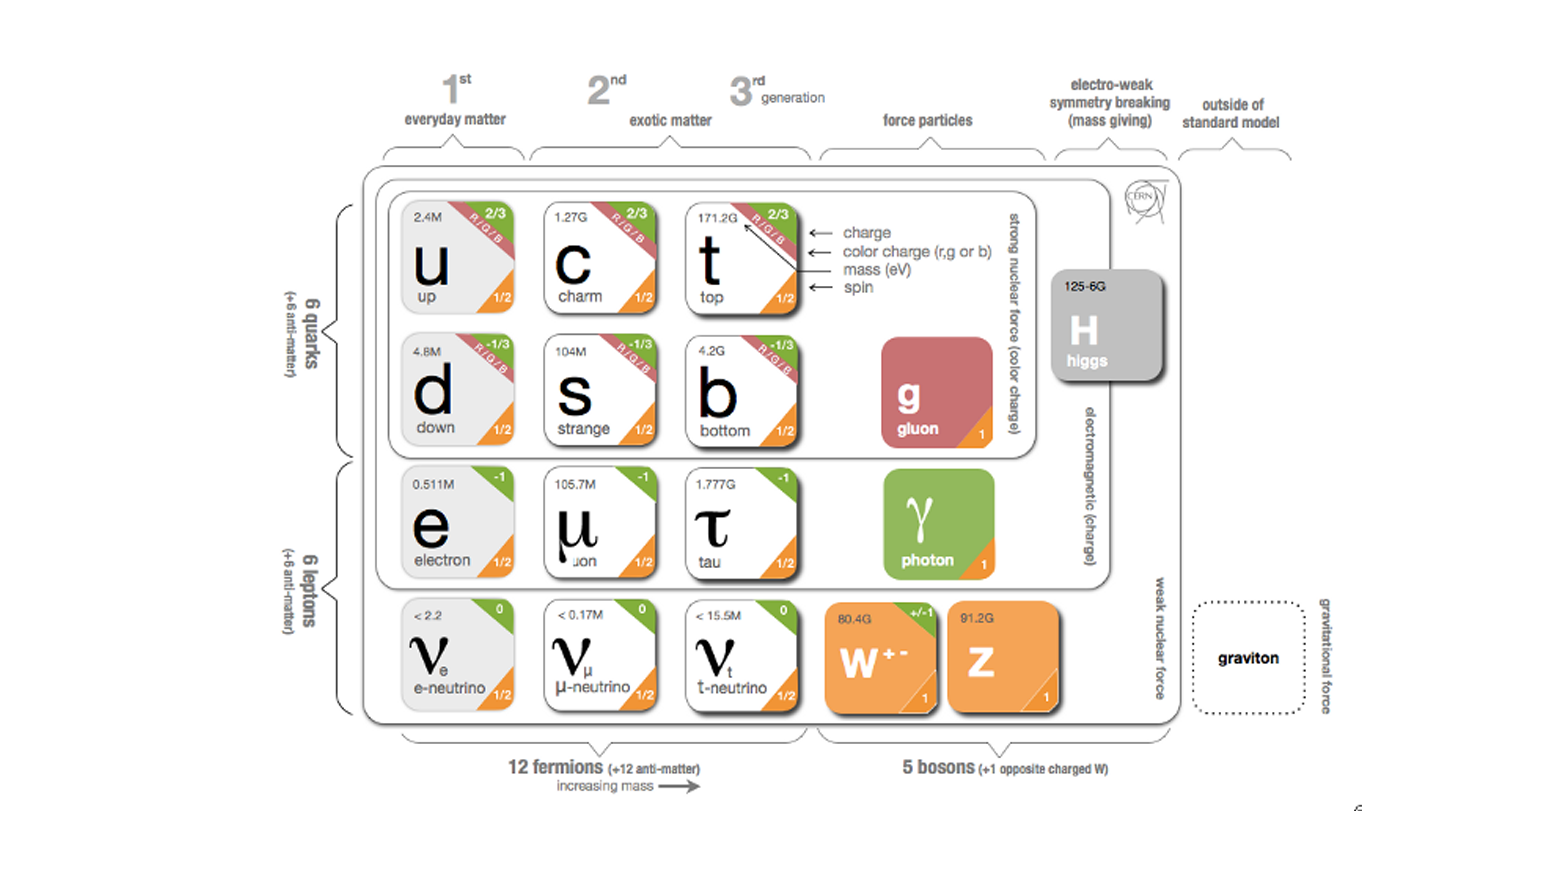
\includegraphics[width = \textwidth]{figures/standardmodel_galbraith_carsten.png}
    \caption{Representation of the standard model of particle physics, highlighting the three main categories of particles (quarks, leptons and force-particles) and the force-particles they interact with~\cite{galbraith_ux_2013}.}
    \label{fig:standard_model}
\end{figure}

The standard model, represented in figure~\ref{fig:standard_model}, consists of six quarks, six leptons, and five force-particles (and all their anti-particles). The force-carrying bosons are exchanged between interacting particles to produce what is perceived as: the strong force mediated by gluons; the electromagnetic force mediated by photons; and the weak force mediated by the charged W-bosons and neutral Z-boson [GRIFFITHS]. The SM actually presents a theory of the electromagnetic and weak force as one force stemming from the same phenomenon: the unified electroweak force [PESKIN]. The Higgs boson field interacts with the particles mediating the unified electroweak force in such a way as to distinguish the weak and electromagnetic forces from each other and give all particles (except neutrinos) a mass. This is referred to as electroweak symmetry breaking [PESKIN]. 

Quarks are fermions that are sensitive to all forces; notably they are the only particles sensitive to the strong force [GRIFFITHS]. Protons and neutrons are made up of quarks and gluons, and the strong force is responsible for their existence and mutual attraction into nuclei [NUCLEAR]. Leptons are particles not sensitive to the strong force. Charged leptons include the electron, which once part of atoms is responsible for chemistry. Neutrinos are neutral, almost massless particles that only interact through the weak force [GRIFFITHS]. 

Common matter is made up of the lightest constituents of the standard model: up and down quarks, electrons and photons. The other particles are or were generated in high-energy environments and decay eventually to the lightest constituents. Such high energy environments include the Big Bang [BIG ORANGE BOOK], astrophysical sources, and accelerators [REV PART PHYS, GRIFFITHS]. The presence of the particles of the standard model at the beginning of the Universe means that their interactions and decays are fundamental for the study of the origin of the Universe [BIG ORANGE BOOK]. Many high energy astrophysical sources, like supernovae, generate particles that rain down on Earth as cosmic rays~\cite{boezio_chemical_2012} [BOEZIO, REV PART PHYS, GRIFFITHS]. Finally, accelerators were built to create controlled high energy environments where the fundamental particles can be produced, detected and subsequently studied [GRIFFITHS, REV PART PHYS].

% --------------------------------------------------
\section{Beyond the Standard Model}
% --------------------------------------------------

The SM provides no explaination for several open questions in particle physics.

First, the fundamental force of gravity is not included in the SM. One might expect a force particle to exist that mediates the gravitational force, but the weak strength of the gravitational force means the graviton will elude detection for a very long time. Moreover, there is no theory of gravity that does not require dark energy or dark matter~\cite{zyla_review_2020}. The universe is expanding at a rate irreconcilable with the known energy density of the Universe, and the nature of this "dark energy" is unknown [BIG ORANGE BOOK]. Dark matter is the name given to mass in the universe whose gravity is measurable, but for which there is no SM explanation~\cite{munoz_dark_2004}.

Second, neutrinos in the standard model are massless; they do not interact with the Higgs field [PESKIN]. However, in 2013 neutrino oscillations were confirmed, which can only occur if neutrinos do have mass~\cite{aharmim_combined_2013}. 

Third, the unification of the electromagnetic and weak force begs the question of if there is a Grand Unified Theory that includes the strong force. 

Theories beyond the standard model (BSM) aim to answer these questions. Often, BSM theories predict new particles. For example, super symmetry (SUSY) predicts that each SM particle has a heavier super symmetric partner. SUSY would explain the origin of dark matter with weakly interacting massive particles and BLANK. Ideally, a BSM theory predicts a measurable signature that can be search for at accelerators or elsewhere.

% --------------------------------------------------
\section{Studying high energy particle physics with accelerators}
% --------------------------------------------------

Accelerators of increasingly high energy have a long history of enabling the discovery of new particles [GRIFFITHS]. Only calling on one example, one of the main goals when the Large Hadron Collider and the ATLAS experiment were proposed was to detect the long-predicted Higgs boson particle~-- a triumph accomplished in YEAR. Being the last particle of the Standard Model to be discovered, the discovery marked the completion of the standard model as it is known today.

Since then, measurements of the cross section of particle physics processes have been enabled by the LHC that test our understanding of the standard model and provide hints of where to look for new physics. A summary of the cross sections measurements done at the ATLAS experiment is shown in figure~\ref{fig:atlas_cross_sections}.
\begin{figure}
    \centering
    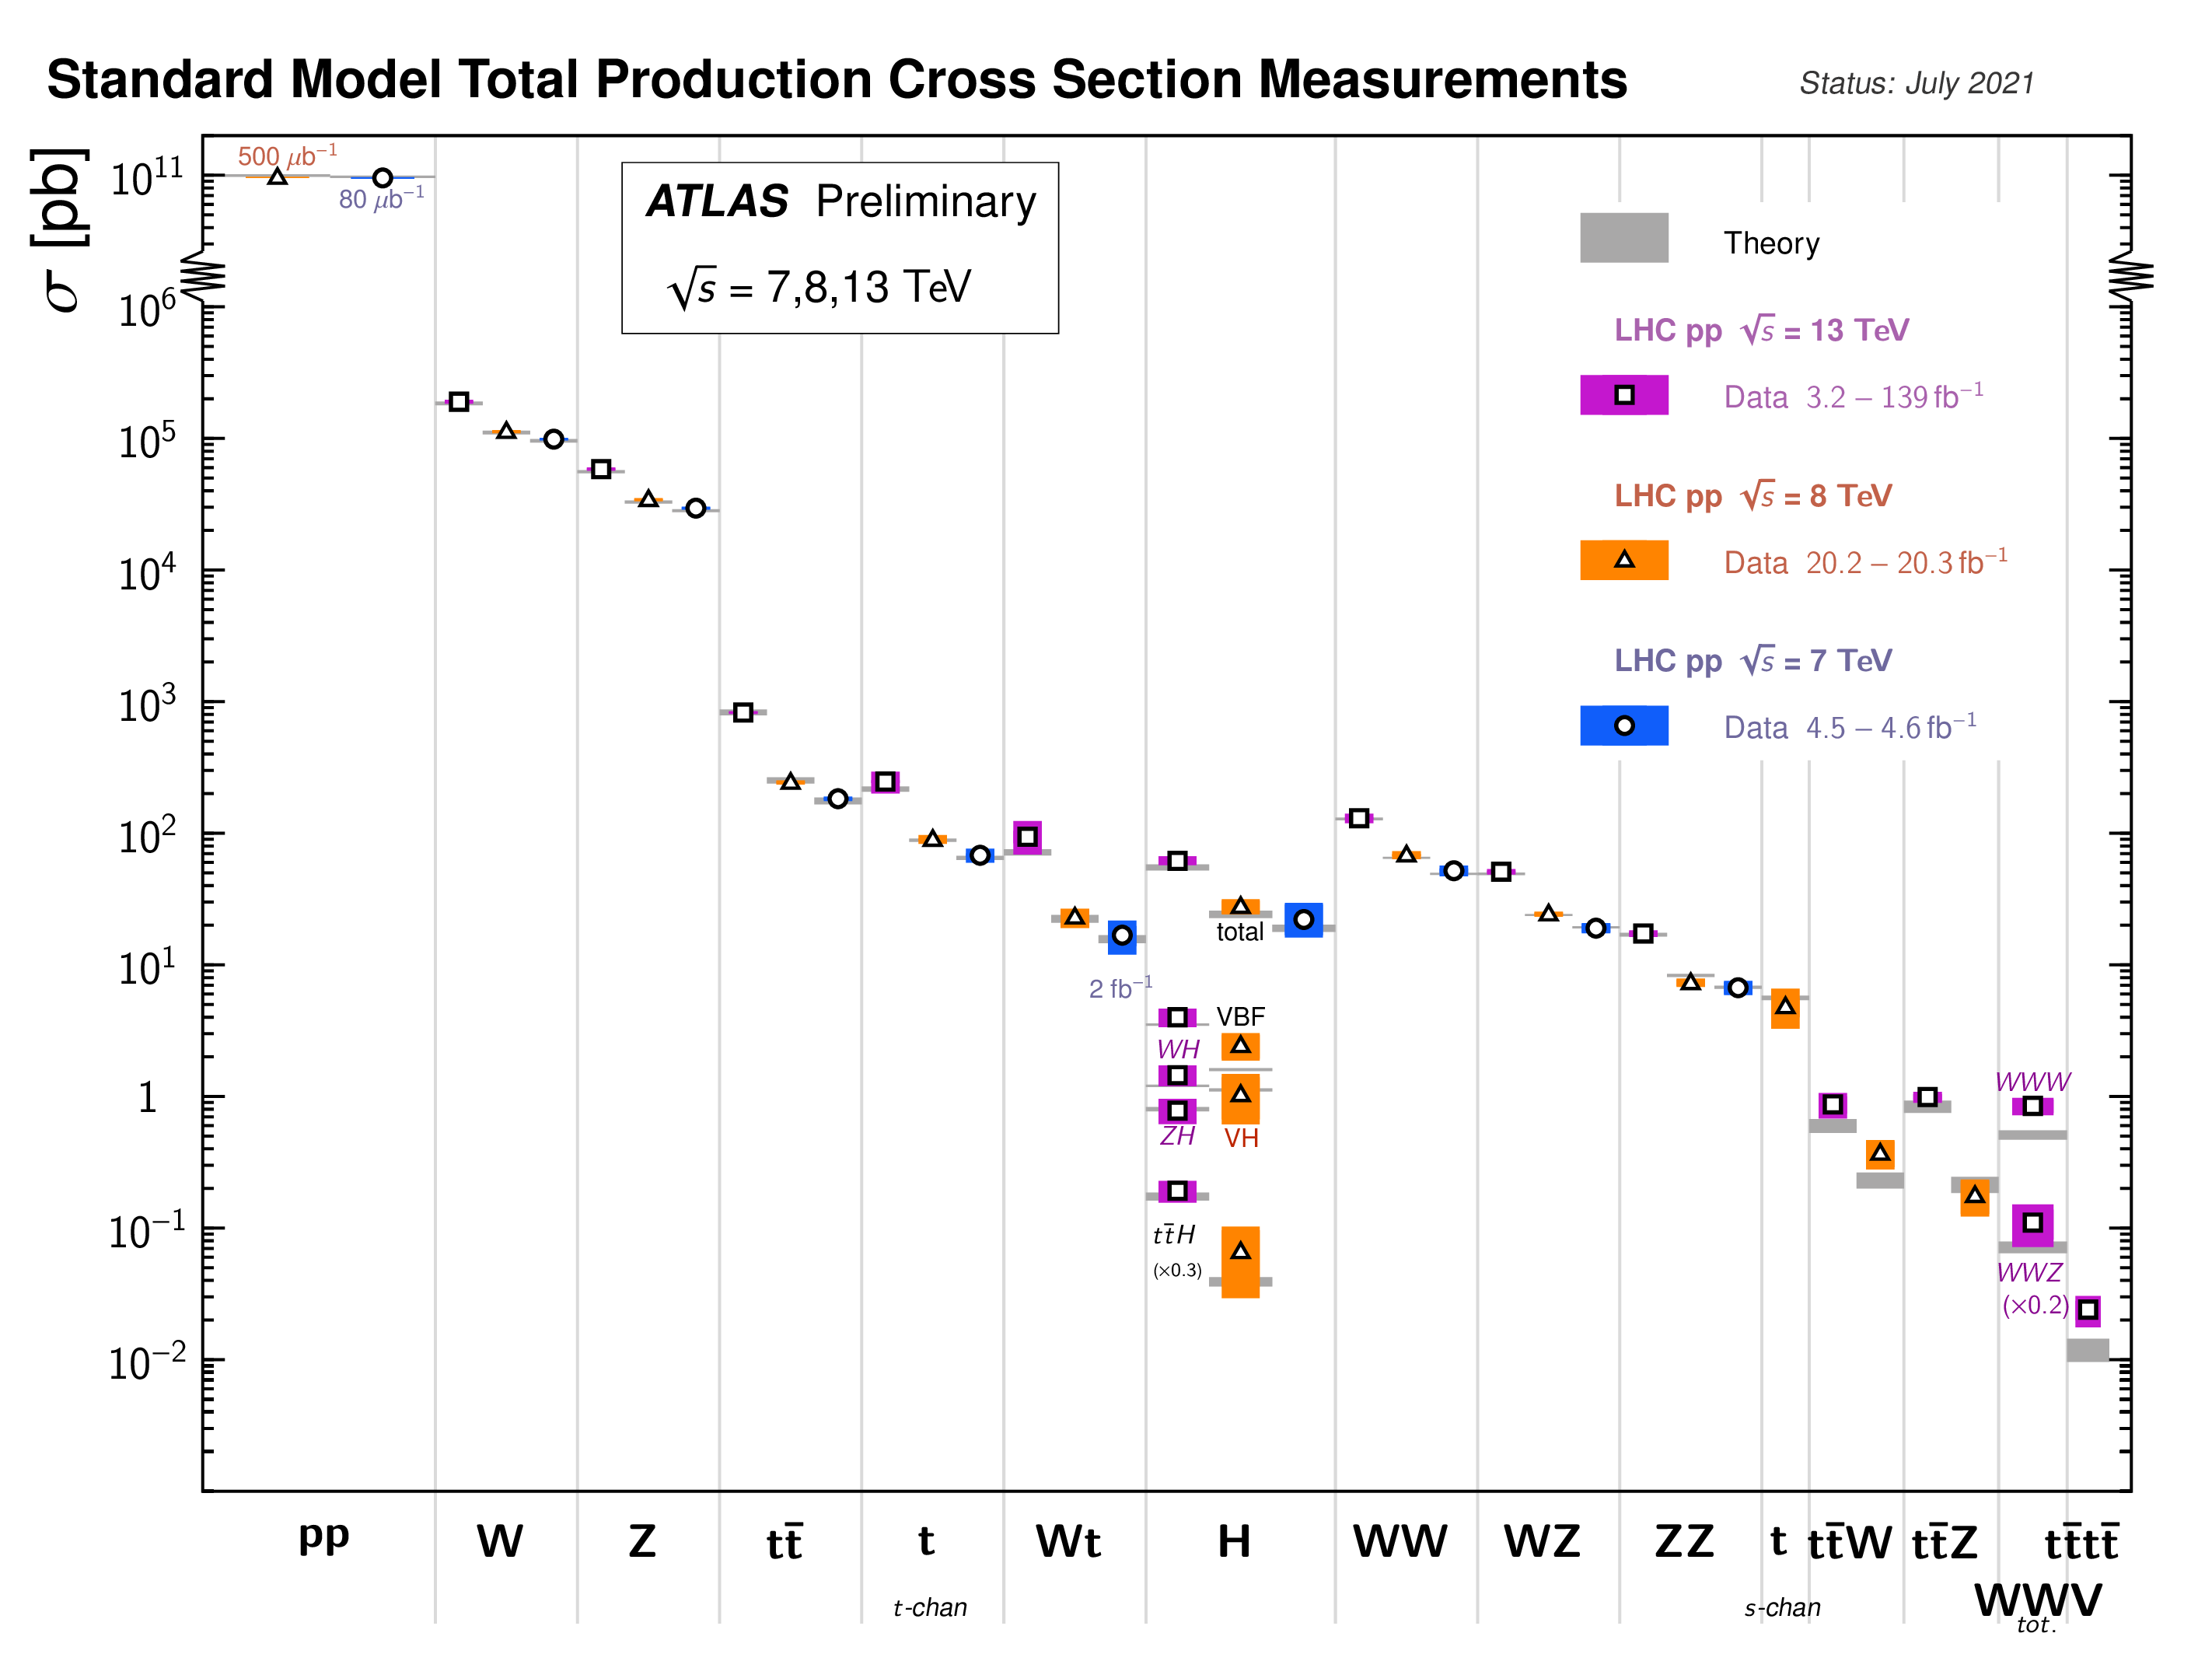
\includegraphics[width = \textwidth]{figures/atlas_cross_sections.png}
    \caption{Cross sections of select SM physics interactions measured using the ATLAS experiment at the LHC. The comparison with theoretical predictions is also shown~\cite{atlas_public_web_sm}.}
    \label{fig:atlas_cross_sections}
\end{figure}

Given the precision to which SM parameters like cross sections have been measured, any discrepancy between theory and experiment could be a portal to new physics tackling the biggest questions in particle physics today. 

Accelerators and detectors can also be used to search for signatures of BSM theories. The controlled, high rate environment enables the search for rare processes that would be impossible to discern in other environments. If the signature is not found, exclusion limits can be set. [EXAMPLE OF FAMOUS ATLAS SEARCH].

Overall, accelerators play a key role in making precision measurements, searching for rare processes predicted by the SM, and testing BSM theories.

% --------------------------------------------------
\section{The Large Hadron Collider}
% --------------------------------------------------

% Include order for inst lum.
% Include bunch crossing frequency
The LHC is an accelerator \SI{27}{\kilo\meter} in circumference and located $\sim$\SI{100}{\meter} underground at CERN near Geneva, Switzerland~\cite{evans_lhc_2008}. It has two beam pipes that counter-circulate bunches of protons\footnote{the LHC also accelerates lead ions, but this paper is written in the context of proton-proton collisions} before colliding the bunches in the center of one of four major experiments, such as the ATLAS experiment (discussed in section~\ref{sec:atlas}). There, the partons interact and many physics processes can occur. The LHC enables physicists to study particle physics at the energy frontier. In the previous run of the LHC (run-2), protons were collided with a center of mass energy of \SI{13}{\tera\electronvolt}. 

% There are two main branches of study that can be pursued with the LHC and ATLAS. First, properties predicted by the standard model (SM) of particle physics can be measured. Else, physicists can search for evidence of processes predicted by theories beyond the standard model. Both the SM measurement and search analyses are based on measuring the number of times a given process occurs and comparing it to expectations. In this way, the number of proton-proton interactions created by the LHC directly affects the statistics available to do SM measurements and searches using the ATLAS experiment.

The number of proton-proton interactions generated by the LHC directly affects the statistics available to make fundamental measurements of cross sections, event rates, etc. 
%IF YOU DON'T NEED TO DEFINE LUMINOSITY
% The number of interactions is quantified by luminosity, a property of the accelerator and its operating conditions~\cite{zyla_review_2020}. When the instantaneous luminosity is integrated over a data collection period and multiplied by the cross section of a given process, the result is the expected number of times that process occurs (so luminosity has units of inverse cross section). Since luminosity is derived from the accelerator parameters, it is the link between the machine and the statistical power of potential measurements. 
% IF YOU NEED TO DEFINE LUMINOSITY
% THIS SECTION IS NOT CITED, probably cite wiht zyla_review_2020
Predicting the number of proton-proton interactions requires defining a metric called luminosity~\cite{zyla_review_2020}. It is the number of particles an accelerator can send through a given area per unit time. It is calculated from the measurable quantities in equation~\ref{eqn:inst_lum}.

\begin{equation}
\mathcal{L} = \frac{f N_{1} N_{2} }{4 \pi \sigma_{x} \sigma_{y}}
\label{eqn:inst_lum}
\end{equation}

In equation~\ref{eqn:inst_lum}, $f$ is the frequency of the bunch crossings (\SI{25}{\nano\second}), $N_{1}$ and $N_{2}$ are the number of protons in each bunch ($\sim 10^{11}$ protons / bunch), and $\sigma_{x}$ and $\sigma_{y}$ are the RMS of the spatial distributions of the bunch. Therefore, luminosity is a property of the accelerator and its operating parameters. The design luminosity of the LHC was $10^{34}$ cm$^{-2}$s$^{-1}$. The units of luminosity are an inverse area; multiplying the luminosity by the cross section of a given process gives the expected rate for that process.

Integrating the \textit{instantaneous} luminosity (equation~\ref{eqn:inst_lum}) over a period of data collection gives the integrated luminosity,

\begin{equation}
L = \int \mathcal{L} \left( t \right) \,dt
\label{eqn:int_lum}
\end{equation}

which is related to the total number of interactions. In this way, the luminosity is the link between the accelerator and the statistical power of measurements to be made with the data collected. Spo far, the LHC provided an integrated luminosity of \SI{28.26}{\per\femto\barn} in run-1~\cite{atlas_luminosity_run1} and \SI{156}{\per\femto\barn} in run-2~\cite{atlas_luminosity_run2}.

% --------------------------------------------------
\section{The High-luminosity LHC}
% --------------------------------------------------

The HL-LHC upgrade~\cite{hl_lhc_tdr} was accepted because without increasing the luminosity of the LHC tenfold, running the accelerator will not provide significant statistical gain on measurements. Also, some systems will need repair and replacement to operate past $\sim$2020. The LHC will be the most energetic accelerator in the world for years to come and is the only accelerator capable of directly producing the Higgs boson and top quarks, so the European Strategy for Particle Physics made it a priority ``to fully exploit the physics potential of the LHC'' with ``a major luminosity upgrade''~\cite{european_strategy_for_particle_physics}. The goal is for the HL-LHC to provide an integrated luminosity of \SI{3000}{\per\femto\barn} in the 12 years following the upgrade. The luminosity actually achieved will depend on a combination of technological advances and upgrades in progress that affect the factors contributing to luminosity defined in equation~\ref{eqn:inst_lum}~\cite{hl_lhc_tdr}.

\begin{figure}
    \centering
    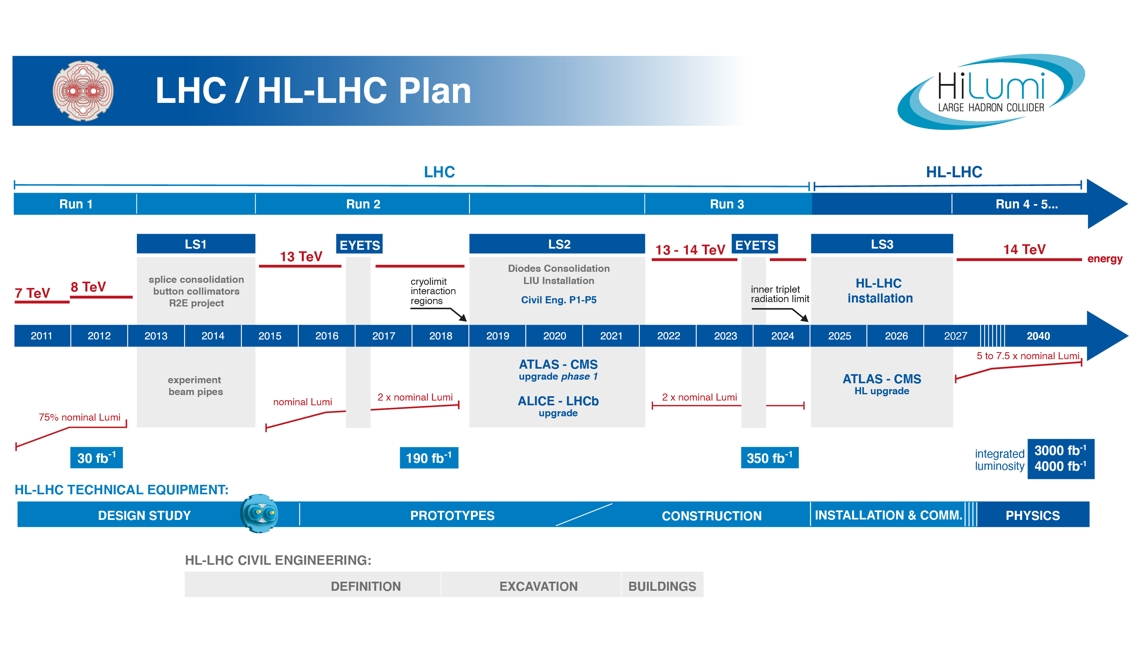
\includegraphics[width = \textwidth]{figures/HL-LHC-updated-January-2021_small.jpg}
    \caption{LHC/HL-LHC plan~\cite{hl-lhc_plan_picture_website}. The integrated luminosity collected and projected for each run of the LHC is shown in red below the timeline and the center of mass energy of the collisions is shown in red above the timeline. The top blue arrow labels the run number. ``LS'' stands for ``long shutdown'' and indicates periods where the accelerator is not operating. During the shutdowns, upgrades to the LHC and the experiments are being installed. This timeline was last updated in January, 2021, and reflects changes in the schedule due to the ongoing pandemic. }
    \label{fig:hl-lhc}
\end{figure}

% The increase in statistics the HL-LHC will improve measurements of standard model parameters and improve searches for unobserved phenomena~\cite{dainese_physics_2018}. A particular measurement that will benefit from the increased statistics is of the triple-Higgs coupling. Measuring the coupling measures the shape of the Higgs potential responsible for electroweak symmetry breaking. Any discrepancy with the SM prediction will show that there must be other sources of electroweak symmetry breaking~-- if there is such another source, it could be an avenue to study the other questions the SM does not address. Also, the sensitivity to several exotic Higgs decays to BSM particles will be improved. Many of the products of exotic Higgs decays are dark matter candidates or otherwise could extend the scope of the SM.

% Higgs couplings to particles will all be measured to the percent level at the HL-LHC and sensitivity to SM predicted Higgs decays will increase. Also, the sensitivity to several exotic Higgs decays to BSM particles will be improved. Many of the products of exotic Higgs decays are dark matter candidates or otherwise could extend the scope of the SM. The LHC is the only accelerator energetic enough to directly produce Higgs bosons, so it is the only tool able to probe questions about the Higgs.

% A particular measurement of interest is of the triple-Higgs coupling. Measuring the coupling measures the shape of the Higgs potential responsible for electroweak symmetry breaking. Any discrepancy with the SM prediction will show that there must be other sources of electroweak symmetry breaking, and hence currently unpredictable particles. Given that the LHC is the only accelerator where the Higgs can be produced directly, it is the only place on Earth where the coupling could be measured.
%The estimated number of interactions of a given type per bunch crossing is given by equation~\ref{eqn:num_interactions}.
%\begin{equation}
%\mu = \sigma \delta t\mathcal{L}
%\label{eqn:num_interactions}
%\end{equation}

% The energies accessible by the accelerator make it unique infrastructure with which to study processes of the standard model of particle physics and search for new phenomenon beyond the standard
% model. Considerable progress has been made towards answering the questions originally used to motivate the construction of the LHC, but many remain unanswered or only partially answered~ \cite{brianti_large_1984}. Therefore, the continued use and maintenance of the accelerator 

% --------------------------------------------------
\section{The ATLAS experiment}
% --------------------------------------------------
\label{sec:atlas}

The ATLAS experiment~\cite{collaboration_atlas_2008} was designed to support all the physics goals of the LHC. It is \SI{44}{\meter} long and \SI{25}{\meter} in diameter, and weighs 7000 tones. It is an array of particle detector subsystems arranged concentrically around the beam pipe and centered around one of the LHC's interaction points (a place where the beams collide), as shown in figure~\ref{fig:atlas}. ATLAS is cylindrical because it aims to provide 4$\pi$ coverage aound the interaction point. It is helpful to separate the subsystems of ATLAS into the so-called ``barrel'' and ``endcap'' or ``forward'' regions.  % <- maybe move this sentence to muon spec section

\begin{figure}
    \centering
    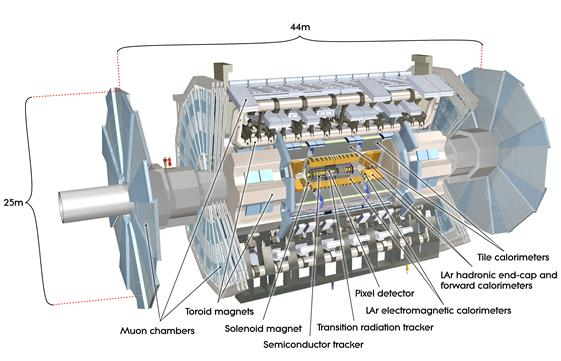
\includegraphics[width = \textwidth]{figures/atlas_diagram.png}
    \caption{Diagram of the ATLAS experiment, with the various detector subsystems labelled. Figure from~\cite{collaboration_atlas_2008}, which also contains more details about the ATLAS experiment.}
    \label{fig:atlas}
\end{figure}

For analysis, ATLAS is typically described in spherical coordinates. The azimuthal angle $\phi$ is measured around the beampipe and the polar angle $\theta$ is measured from the beam pipe. A more useful coordinate than $\theta$ is the pseudo-rapidity, $\eta = -\ln\tan\left(\theta/2\right)$, because it approaches the rapidity of a particle when its momentum is much greater than its mass and differences in rapidity are approximately invariant to a Lorentz boost parallel to the beam. The range of $\eta$ is 0 (perpendicular to the beam) to $\pm\infty$ (parallel to the beam, or the z-direction). Typically, $\eta$ is the physically interesting coordinate because the $\phi$ coordinate follows the cylindrical symmetry of the beam.

It is not actually the proton bunches that collide and generate physics processes, but their constituent partons. Since the partons may carry an unknown fraction of the momentum, ATLAS analyses are based on the sum of the transverse momentum ($p_T$) and energy of outgoing particle being approximately zero (transverse meaning perpendicular to the beam). \textcolor{red}{The goal of ATLAS is to reconstruct the transverse momentum of each collision product to understand what happened in each collision. \textit{-> Do I have this right?}} A brief overview of the sub-systems of ATLAS is given, starting from the system closest to the beam and moving outwards. Each sub-system is responsible for a different group of collision products.

\paragraph*{The inner detector} \hfill \break
The inner detector~\cite{atlas_inner_detector_tdr_1, atlas_inner_detector_tdr_2} (figure~\ref{fig:atlas_inner_detector}) is for precision tracking, vertex measurements and electron identification. A \SI{2}{\tesla} solenoid with field parallel to the beam bends the track of outgoing particles to make momentum measurements possible. The innermost part is made of high-resolution semiconductor pixel and strip detectors for precision tracking while the outermost part are straw-tubes that generate and detect transition radiation for electron identification.

\begin{figure}
    \centering
    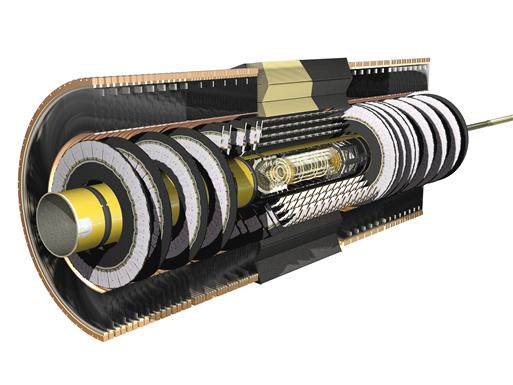
\includegraphics[width = 0.5\textwidth]{figures/atlas_inner_detector.jpg}
    \caption{Diagram of the ATLAS experiment's inner detector, with the different segments and the technology used labelled. Figure from~\cite{collaboration_atlas_2008}.}
    \label{fig:atlas_inner_detector}
\end{figure}

\paragraph*{Calorimetry system} \hfill \break
Electromagnetic and hadronic sampling calorimeter units are used to record the energy of electrons, photons, jets and missing transverse energy (from neutrinos, for example). A combination of liquid-argon (LAr) electromagnetic and hadronic calorimeters~\cite{atlas_lar_cal_tdr} and tile-scintillator hadronic calorimeters~\cite{atlas_tile_cal_tdr} cover the rapidity range $|\eta| < 4.9$, as shown in figure~\ref{fig:atlas_calorimeter}.

\begin{figure}
    \centering
    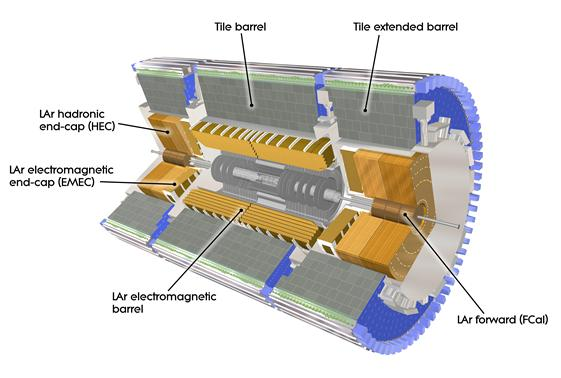
\includegraphics[width = 0.5\textwidth]{figures/atlas_calorimeter.png}
    \caption{Diagram of the ATLAS calorimeter system, with the different segments and the technology used labelled. Figure from~\cite{collaboration_atlas_2008}.}
    \label{fig:atlas_calorimeter}
\end{figure}

The calorimeters cause incoming charged particles to shower and deposit their energy in the sensitive volume. Only muons and neutrinos are known to pass the calorimeters to the muon spectrometer.  Particles other than those mentioned would have decayed in the inner detector before reaching the calorimeter. 

\paragraph*{Trigger system} \hfill \break
It would be impossible to record all the data from bunch crossings every \SI{25}{\nano\second}, corresponding to a rate of $\sim$\SI{40}{MHz}, so ATLAS has a multi-level trigger system to select events of interest for permanent storage. The Level-1 (L1) hardware trigger~\cite{atlas_l1_trigger_tdr} uses partial-granularity information from the muon spectrometer and calorimeter to trigger on high $p_T$ muons, electrons, jets, high missing transverse energy, and $\tau$ decaying to hadrons. The maximum L1 trigger rate ATLAS can accommodate is \SI{100}{kHz} with a latency of \SI{2.5}{\micro\second}. 

% The Level-1 (L1) hardware trigger uses the muon spectrometer's TGCs and RPCs to trigger on high $p_T$ muons and the calorimeter detector units to trigger on electrons, jets, high missing transverse energy, and $\tau$ decaying to hadrons, with a maximum trigger rate of \SI{100}{kHz} and latency of \SI{2.5}{\micro\second}. The L1 trigger only uses a fraction of the granularity offered by the detectors.

The L1 trigger is used to define regions of interest that are fed into the software high level trigger (HLT), in which the full granularity of the muon spectrometer and calorimeter are used with information from the inner detector to reduce the trigger rate to 1 kHz. Events that pass the L1 and HLT trigger are recorded for use in offline analysis~\cite{atlas_hlt_trigger_tdr}.

The ATLAS trigger system is described in the references above but the trigger rates quoted here are after the upgrades implemented for run-2, described in~\cite{martinez_run-2_2016}.

\paragraph*{Muon spectrometer} \hfill \break
Magnetic deflection by superconducting air-core toroid magnets is used to measure muon momentum and energy. In the barrel of ATLAS, eight coils bent into ``racetracks'' are arranged around the beampipe provide the magentic field. In the forward region, two end-cap toroids each with eight smaller racetrack-shaped coils arranged symmetrically around the beampipe are inserted in the ends of the barrel toroid~\cite{atlas_magnet_tdr}. Figure~\ref{fig:atlas_muon_spectrometer} shows the toroid magnets and the different parts of the ATLAS muon spectrometer.

\begin{figure}
\centering
\begin{subfigure}{.5\textwidth}
  \centering
  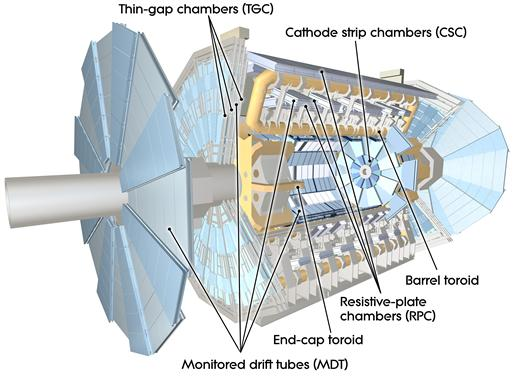
\includegraphics[width=\linewidth]{figures/atlas_muon_spectrometer.jpg}
  \caption{}
  \label{fig:atlas_muon_spectrometer_3D}
\end{subfigure}%
\begin{subfigure}{.5\textwidth}
  \centering
  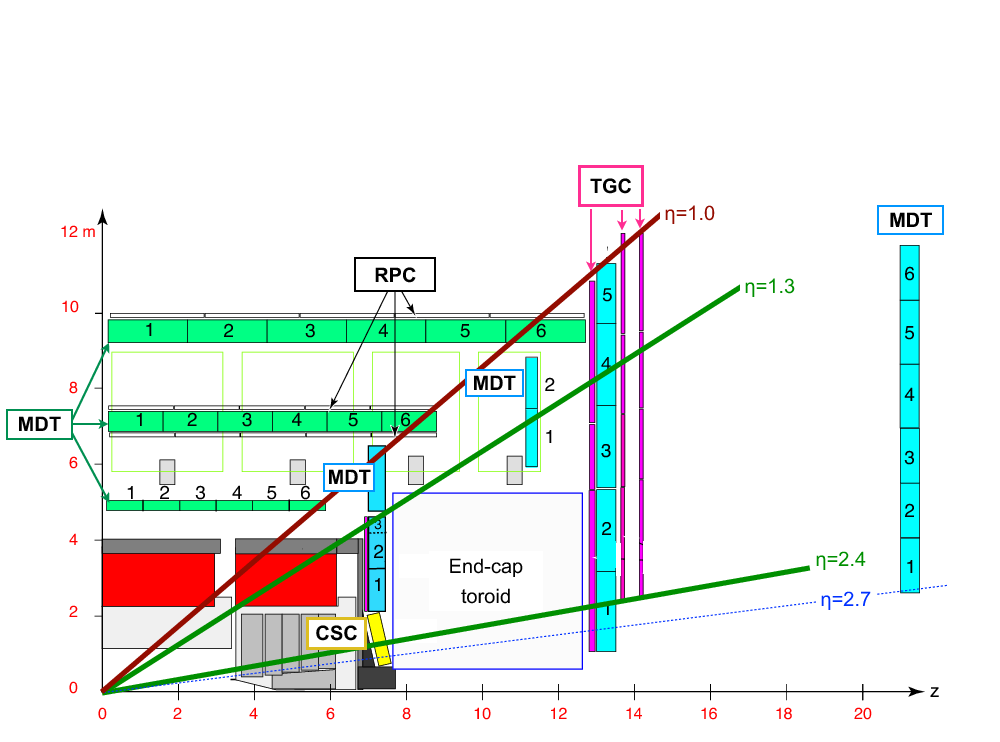
\includegraphics[width=\linewidth]{figures/atlas_old_muon_spec_quarter_cut_recolour.png}
  \caption{}
  \label{fig:atlas_muon_spectrometer_cut}
\end{subfigure}
\caption{(a) The ATLAS muon spectrometer~\cite{collaboration_atlas_2008}. (b) A quarter-cut of ATLAS, with the interaction point in the bottom left corner. The small wheel is just left of the end cap toroid, the big wheel is to its right, and the outer wheel is the rightmost structure~\cite{atlas_performance_muon_trigger_2015}}
\label{fig:atlas_muon_spectrometer}
\end{figure}

The muon spectrometer~\cite{atlas_muon_spectrometer_tdr} is separated into detectors used for precision offline tracking and for triggering. Three layers of monitored drift tubes (MDTs) or cathode strip chambers (CSCs) are used for tracking. The position of the muon track in each of the three layers allows reconstruction of the track sagitta and hence momentum. For the design momentum resolution of $\Delta p_T / p_T <$~1$\times$10$^{-4}~p$~/~GeV for $p_T <$~300~GeV and a few percent for lower $p_T$ muons, the MDTs and CSCs required position resolution of \SI{50}{\micro\meter} each. Accordingly, an optical alignment system was designed to monitor and correct for chamber positions~\cite{atlas_muon_spectrometer_tdr, aefsky_optical_2008}. 

% Precision tracking is done offline for events passing the muon trigger. Each of the barrel and encap systems have three layers of MDTs that record the position of the muon as it passes through each layer. Knowing the magentic field, the muon's momentum can be extracted. For the design momentum resolution of $\Delta p_T / p_T <$ 1$\times$10$^{-4}~p$ / GeV for $p_T < 300 GeV$ and a few percent for lower $p_T$ muons, the MDTs and CSCs required position resolution of \SI{50}{\micro\meter} each. Accordingly, an optical alignment system was designed to monitor and correct for chamber positions~\cite{atlas_muon_spectrometer_tdr, aefsky_optical_2008}. 

% ON MUON TRIGGERING IN THE ENDCAP
% Decide how you want to do this based on the next section.
% At least 2 TGC layers in coincidence comes from muon spectrometer TDR; coincidence with "forward inner" detectors (small wheel) comes from run 2 trigger upgrades paper, Martinez.
% NSW TDR says there are TGC layers in the small wheel that are the forward inner detectors added to run 2 triggering.
% \textcolor{red}{The run 2 L1 muon trigger was passed if TGC layers (two for low $p_T$ muons, three for high $p_T$ muons) of the big wheel fired in coincidence with a hit from the MDTs of the small wheel on the order of the bunch crossing time. The regions of interest defined by the TGCs were fed into the HLT, where MDT and TGC data could be combined for further cuts. The $p_T$ resolution of the L1 trigger is improved by the MDT tracking information. \textit{I'll decide how I want to do this after writing the motivation for the NSW}}
Resistive plate chambers (RPCs) are used for triggering in the barrel and thin-gap chambers (TGCs) are used for triggering in the endcaps. The positions of each type of chamber are sketched in figure~\ref{fig:atlas_muon_spectrometer_cut}. Often, the endcap muon spectrometer is separated into three wheels~-- the small wheel (SW), big wheel, and outer wheel~-- ordered by proximity to the interaction point. In run-1, low (high) $p_T$ muons were triggered on at L1 if two (three) of the RPCs or TGCs layers around the big wheel fired in coincidence, for the barrel and endcaps respectively~\cite{atlas_l1_trigger_tdr}. After run-1 it was discovered that up to 90\% of the triggers in the endcap were fake, caused by background particles generated in the material between the small wheel and the big wheel~\cite{nsw_tdr}.  To reduce the fake rate in run-2, the TGCs on the inside of the small wheel also had to register a hit. The added condition reduced the trigger rate by 50\% in the range 1.3 $< |\eta| <$ 1.9~\cite{martinez_run-2_2016}. The effectiveness of the solution was limited since the $|\eta|$-range of the small wheel TGCs was limited to 1.0 $< |\eta| <$ 1.9 and the position resolution of the small wheel TGCs is coarse~\cite{nsw_tdr}.

% In the barrel, three layers of MDTs are used for precision tracking, and resistive plate chambers (RPCs) are used for triggering. The endcaps of the muon spectrometer are composed of three wheels each, the small wheel (SW), big wheel, and outer wheel. All three wheels use MDTs for precision offline tracking, but cathode strip chambers (CSCs) are used in the forward region of the small wheel because they can better handle the increased background. Thin gap  chambers

% The big wheel and the outer wheel have MDTs for offline precision tracking and the thin gap chambers (TGCs) on either side for triggering. In the first two runs of ATLAS, offline precision tracking on the small wheel was done with MDTs and cathode strip chambers (CSCs), and their output did not contribute to the trigger.~\cite{atlas_muon_spectrometer_tdr}. 

% Sentences if you go without 1/4 cut figure
% In the barrel, three layers of monitored drift tubes (MDTs) are arranged between, above and below the barrel toroid magnets. They are used for precision tracking. On both sides of the middle layer of  MDTs and on the top of the top layer of MDTs are resitive plate chambers (RPCs), used for triggering.
%  The inner part had cathode strip chambers (CSCs), which had higher granularity to handle the increased background radiation rate in the forward region

% The muon spectrometer is the outermost layer of the ATLAS detector, since only muons (and neutrinos) can pass through the calorimeters. For muons that are ejected towards the end-caps of ATLAS, their trajectory is bent by the magentic field and their position recorded by three successive wheels of muon detectors. With each wheel providing the position of the muon along its trajectory and knowledge of the magentic field, the momentum of the muon generated in the collision can be reconstructed. 
% ==================================================
% CHAPTER 3: The New Small Wheels %
% ==================================================

\chapter{The New Small Wheels}
\label{chap:nsw}
% Edit count: Lia - 0, Brigitte - 0

% --------------------------------------------------
\section{Motivation for the New Small Wheels (NSWs)}
% --------------------------------------------------

At the end of the HL-LHC upgrade, there could be up to a sevenfold increase in luminosity~\cite{hl_lhc_tdr}. Simultaneously, the background radiation rate increases linearly with luminosity. The combined rate presents problems for both the tracking and triggering capabilities of the muon spectrometer~\cite{nsw_tdr}.

In term of tracking, the efficiency of the MDTs decreases by 35\% (mostly due to long dead-times) already when exposed to the maximum hit rate at the current luminosity, 300 kHz.
At a threefold increase in luminosity, which is predicted for run 3, most of the SW will be subjected to a hit rate well above 300 kHz. Losing muon hits in the small wheel will reduce the high $p_T$ muon momentum resolution. The decrease in resolution will affect the ability to search for high mass $Z'$, $W'$ and pseudo-scalar Higgs~\cite{nsw_tdr}.

Already, the forward muon trigger system copes with a very high fake rate, even when including TGC data from the SW in the trigger as in run-2. At the luminosity expected in run 3, 60 kHz of the maximum 100 kHz of the L1 trigger would be taken by the endcap muon spectrometer. A possible solution would be to raise the minimum $p_T$ threshold from \SI{20}{\giga\electronvolt} to \SI{40}{\giga\electronvolt}, but the ability to study several physics processes of interest depend on low $p_T$ muons~\cite{nsw_tdr}

The NSW will solve both these problems. It will be covered with precision tracking chambers suitable for the expected hit rates and triggering chambers capable of \SI{1}{mrad} angular resolution. The idea behind the triggering chambers is to match the small wheel track segment with the track segment from the big wheel to discard tracks not originating from the interaction point. Figure~\ref{fig:nsw_track_triggering} illustrates this point: the old trigger system would have triggered on all three tracks, while with the NSW the trigger system would only trigger on track A~\cite{nsw_tdr}.

% Currently, the small wheel is made of thin-gap chambers, which record hits. They have the known problem that particles generated in the material of the end-cap toroid magnet that hit the small wheel cannot be distinguished from muons from the interaction point. For example, in figure~\ref{fig:nsw_track_triggering}, all three tracks would be triggered on.

\begin{figure}
    \centering
    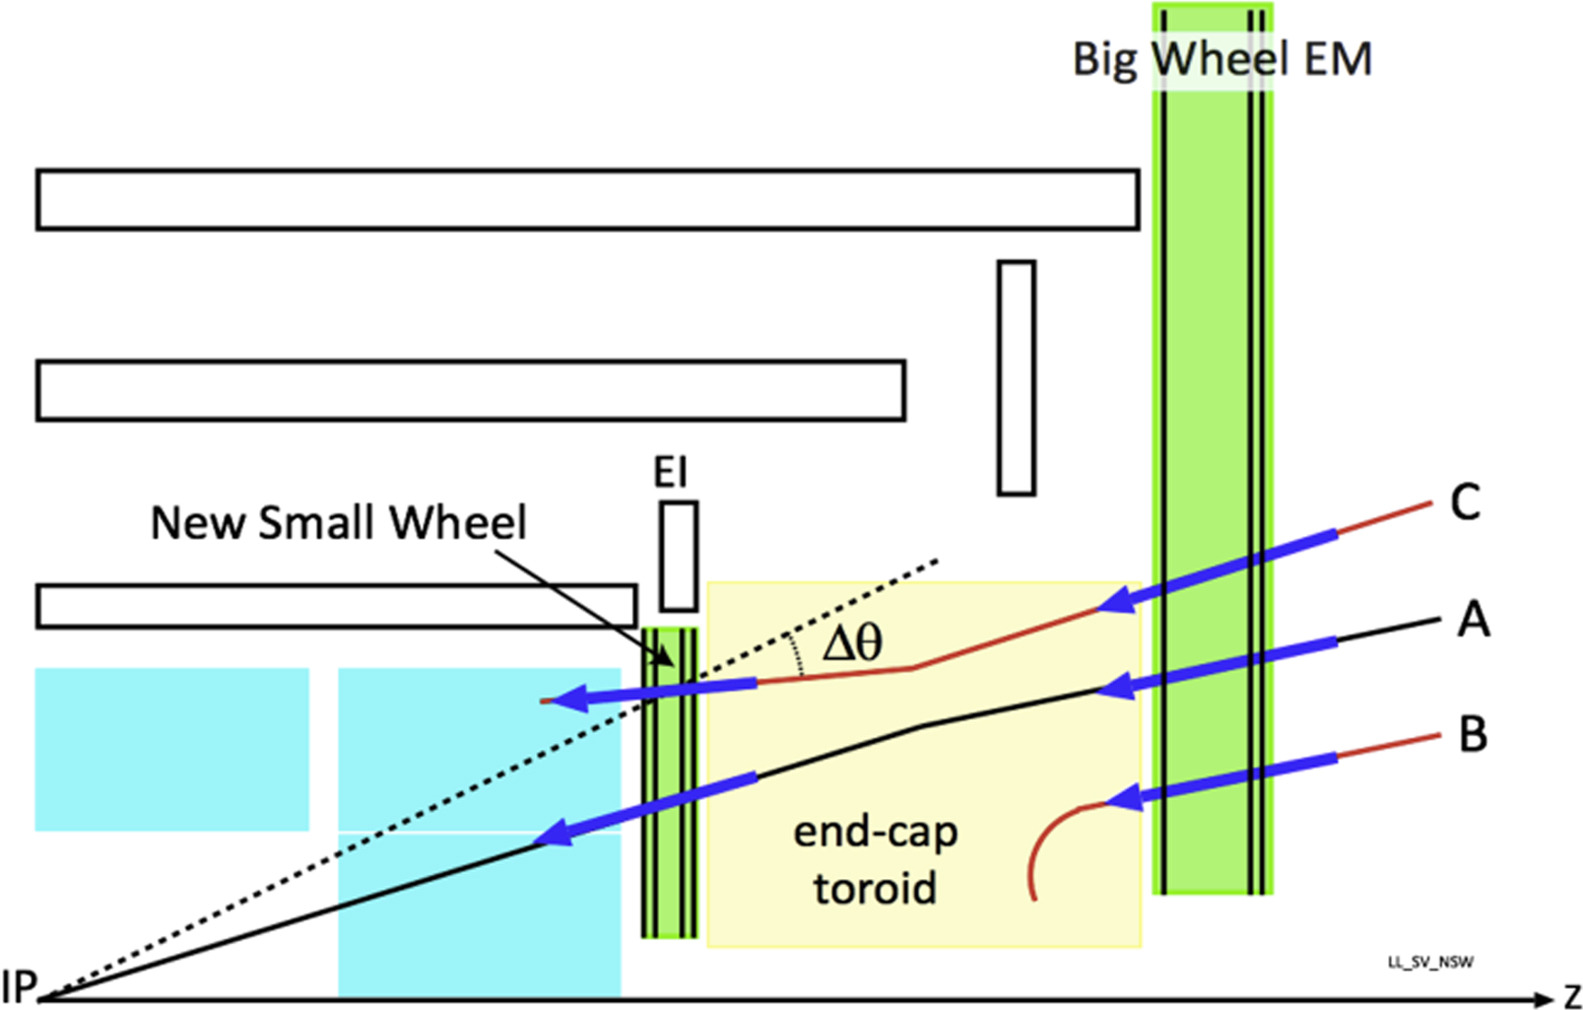
\includegraphics[width = 0.9\textwidth]{figures/perez-codina_NSW_tracks.jpg}
    \caption{A schematic of a quarter cross section of the ATLAS detector, with the collision/interaction point (IP) in the bottom left corner. Three possible tracks are labelled. Ideally, track A would be triggered upon while track B and C discarded. With the small wheel, all three tracks would be recorded. With the new small wheel, only track A would be recorded~\cite{nsw_tdr}.}
    \label{fig:nsw_track_triggering}
\end{figure}

% --------------------------------------------------
\section{Design of the NSWs}
% --------------------------------------------------

The NSWs are covered with two detector technologies: micromegas (MM) and small-strip thin gap chambers (sTGCs). MMs are the primary tracking detectors and sTGCs are the primary triggering detectors, but for redundancy sake both are designed to do either. As such, both sets of detectors are to have position resolution better than $\sim$\SI{100}{\micro\meter} per plane. \textcolor{red}{\textit{Is quoting 100 um ok? Originally in the TDR, it was smaller, but given how detector construction has played out I think this is the new working goal}}. Four chambers of each type are glued together to create quadruplet modules. Quadruplets of different sizes are assembled into wedges. Two sTGC wedges and two MM wedges are layered to create sectors (with the sTGC wedges on the outside)~\cite{nsw_tdr}. Different stages of the constrcution process are shown in figure~\ref{fig:nsw_breakdown}.% \textcolor{red}{\textit{for if you use computer generated NSW diagram}} Sectors covered the wheel, as shown in figure~\ref{fig:nsw_diagram}. Practically, two different wedge sizes, small and large, were required to completely cover the wheel.
% \begin{figure}
%    \centering
%    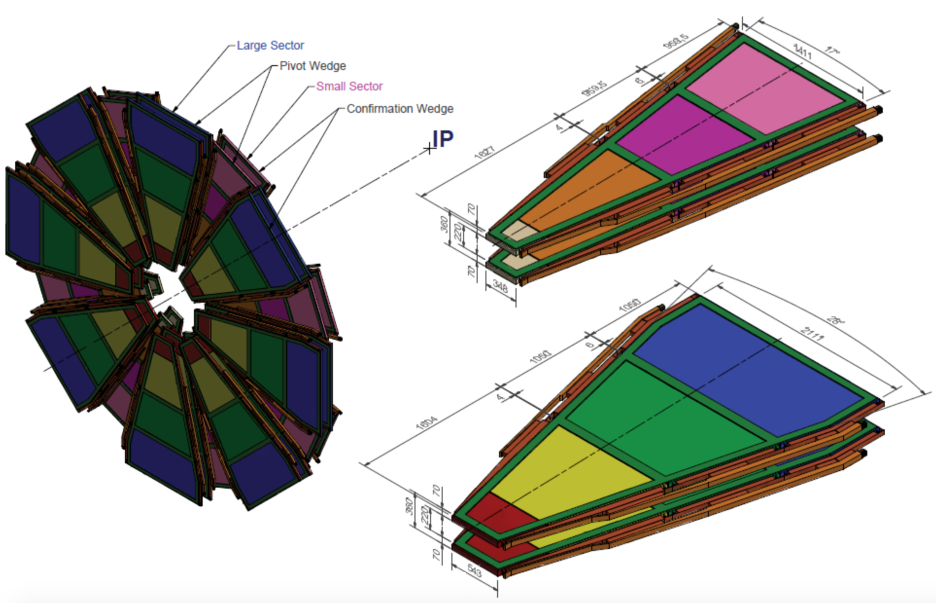
\includegraphics[width = 0.9\textwidth]{figures/nsw_diagram.png}
%    \caption{Drawing of the new small wheel, and diagrams of the individual small and large wedges. Each colour represents a different sTGC module size.}
%    \label{fig:nsw_diagram}
% \end{figure}
\newpage
\thispagestyle{empty}
\newgeometry{top=0.5in,bottom=0.5in}
\begin{figure}
\centering
\begin{subfigure}{\textwidth}
  \centering
  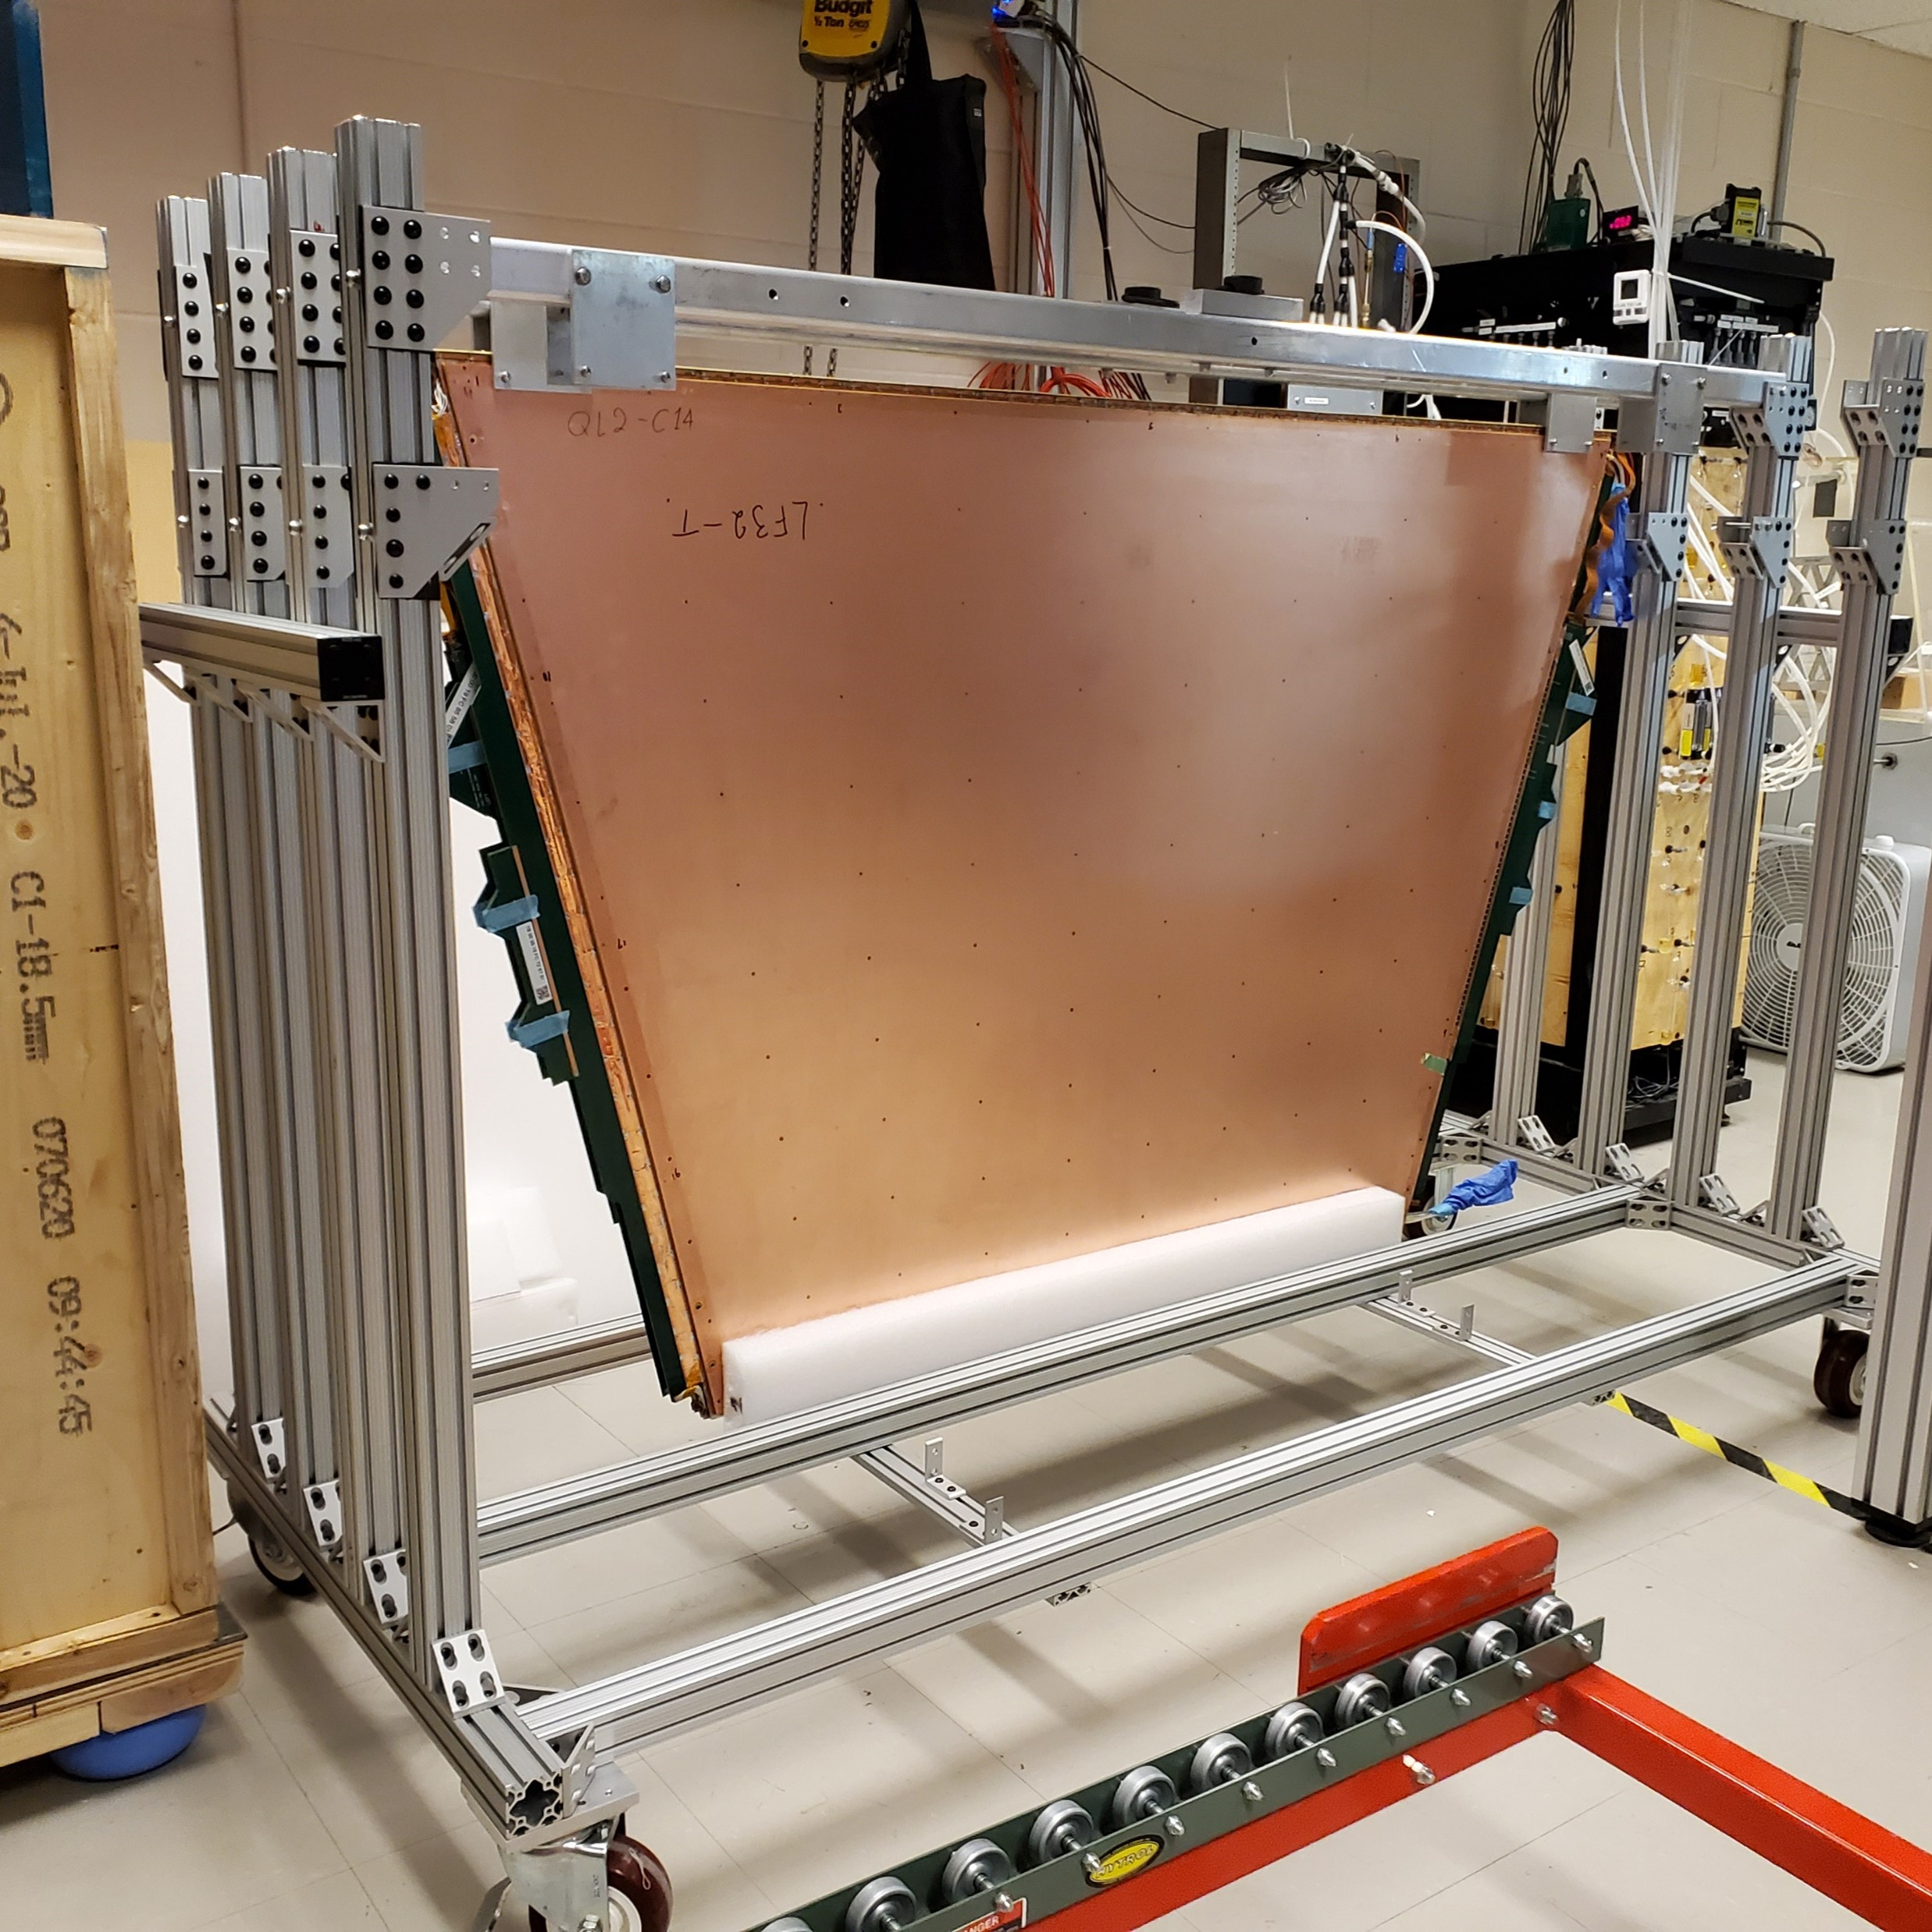
\includegraphics[width=0.35\textwidth]{figures/stgc_quad_cart.jpg}
  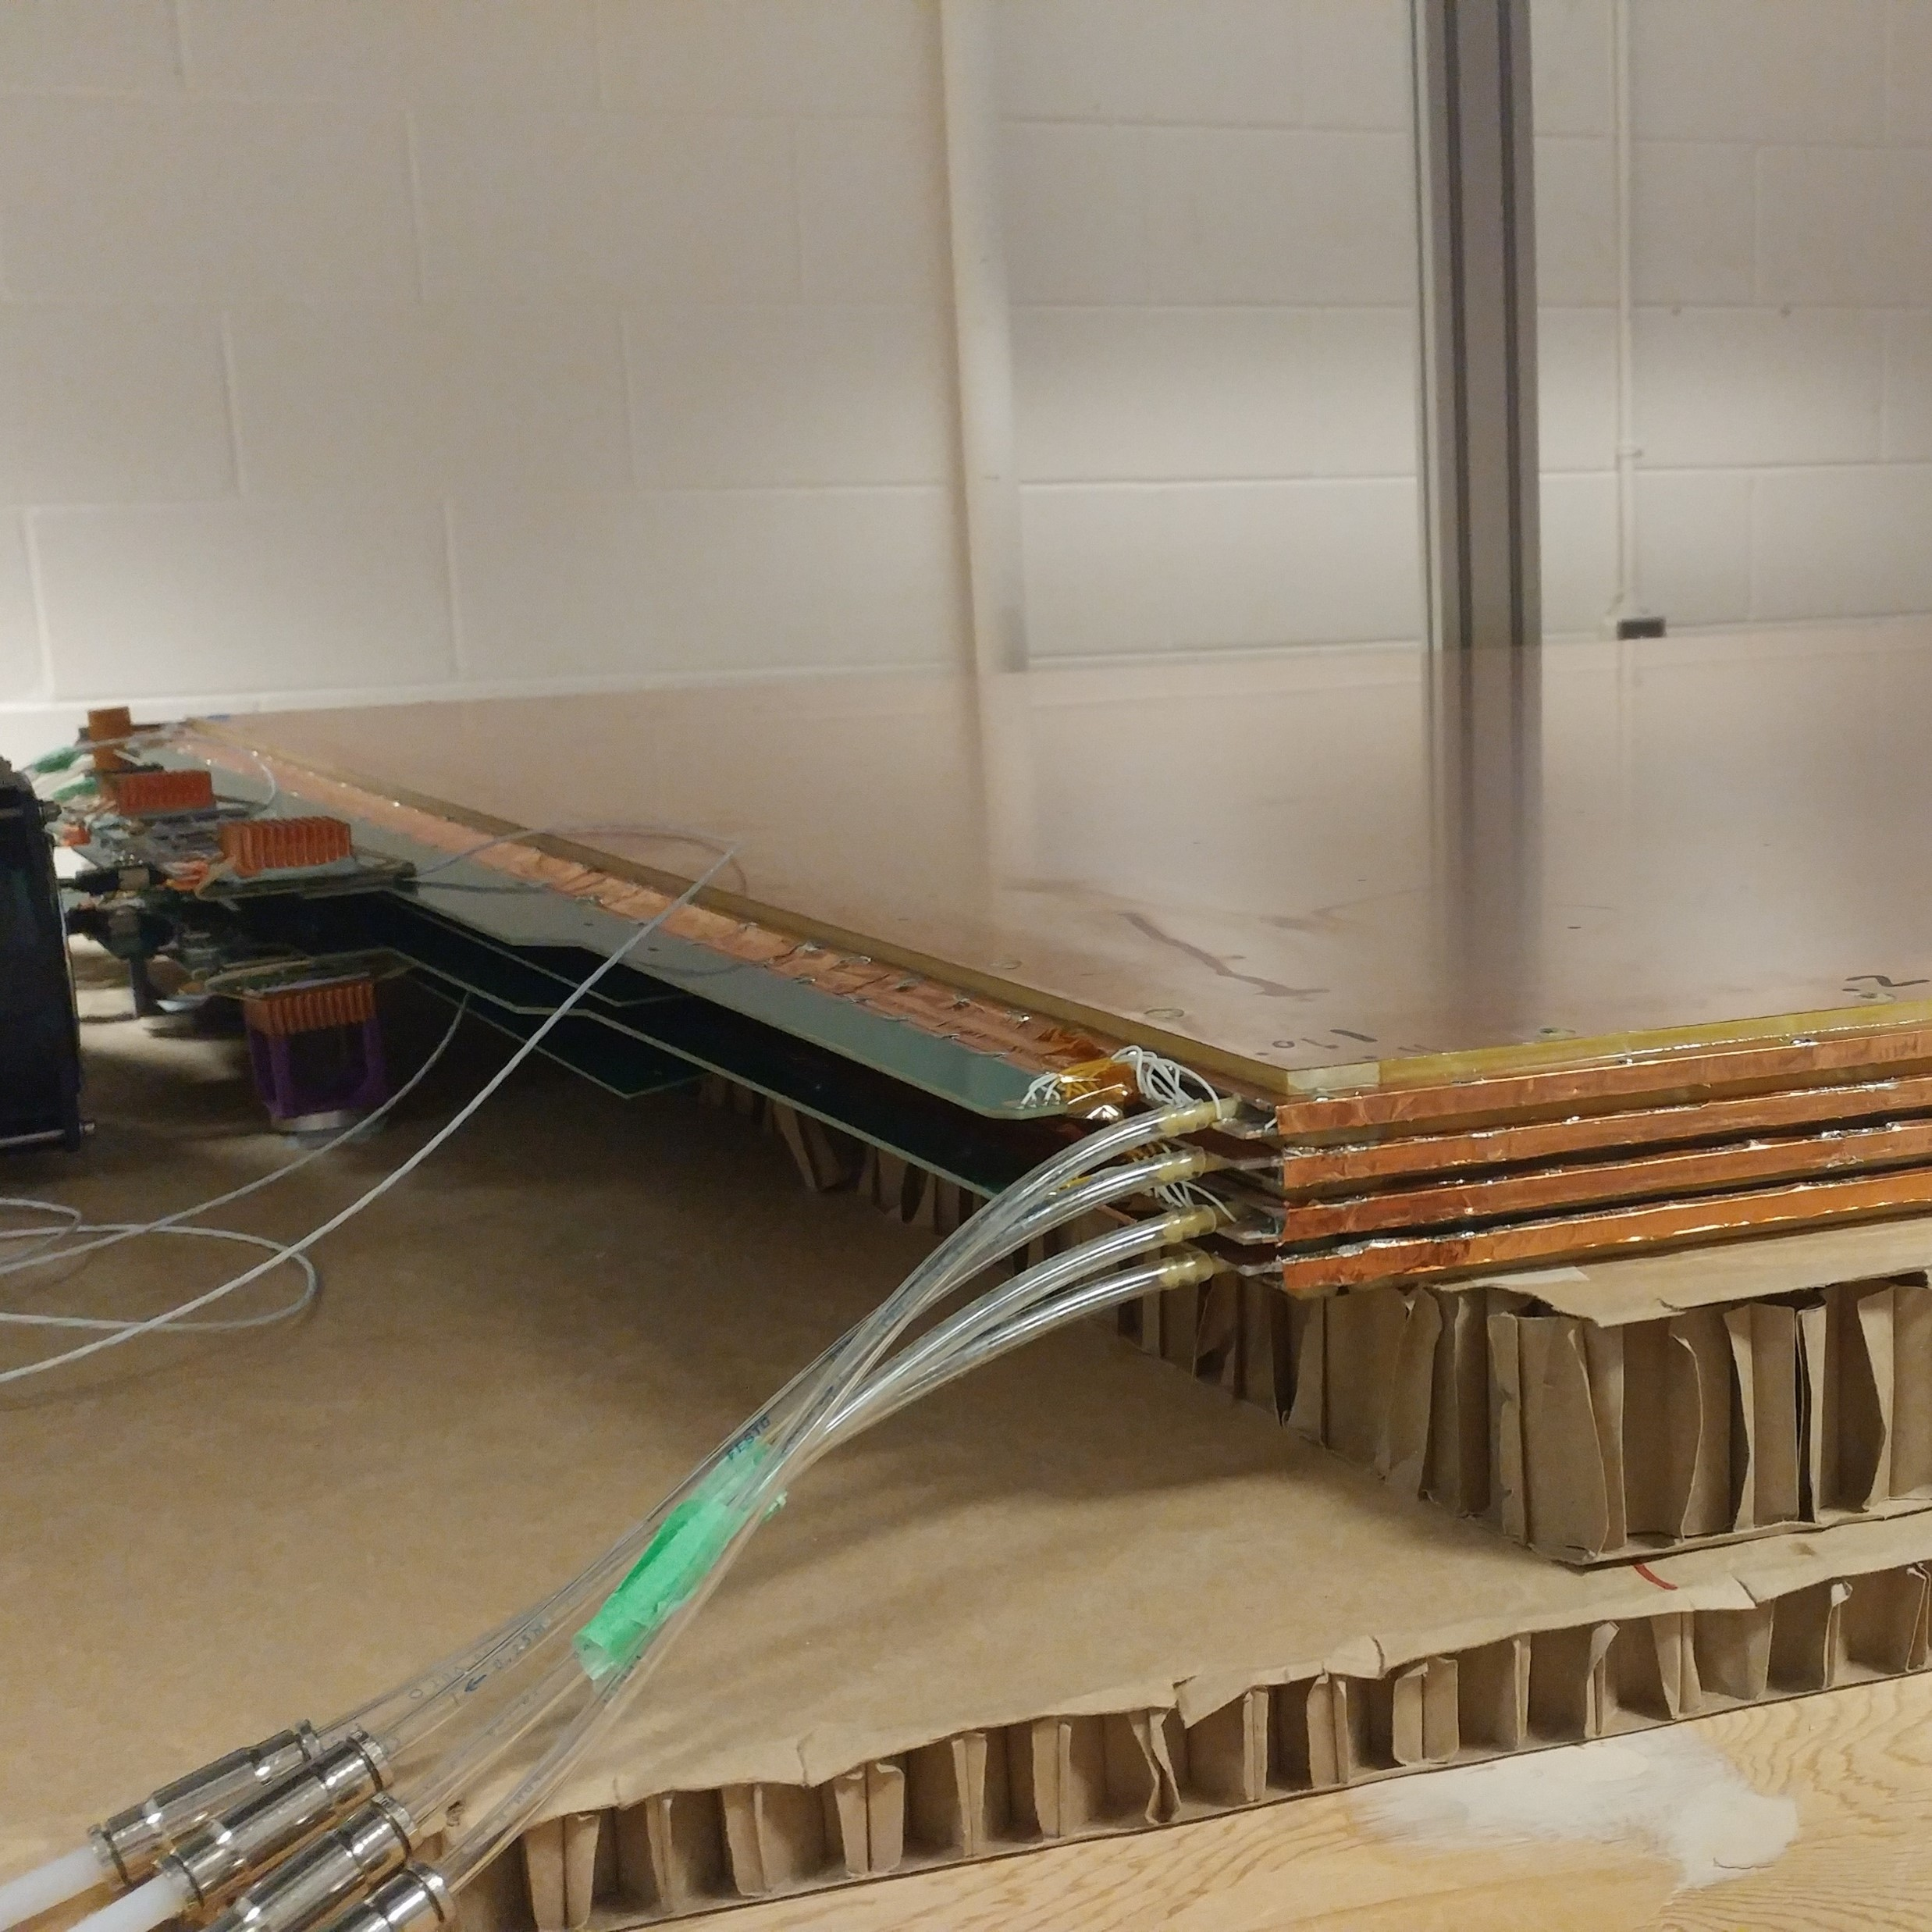
\includegraphics[width=0.35\textwidth]{figures/stgc_quad_inlet_corner.jpg}
  \caption{An sTGC quadruplet module. The left image highlights the trapezoidal shape. The right image shows the short edge corner, highlighting the four sTGC layers and each layer's gas inlet. The gas outlets and high voltage cables are at the long edge in the back of the photo. The green printed circuit board along the sides are the adaptor boards where the front end electronics are attached.}
  \label{fig:stgc_quad}
\end{subfigure}

\smallskip

\begin{subfigure}{\textwidth}
  \centering
  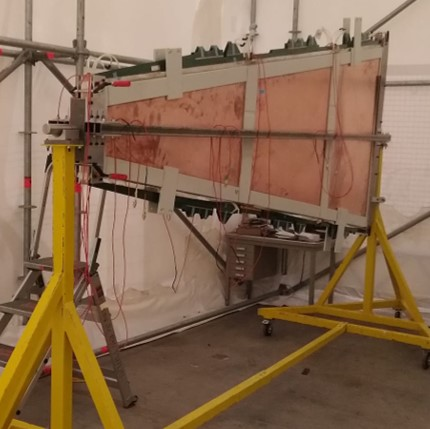
\includegraphics[width=0.35\textwidth]{figures/stgc_wedge.jpg}
  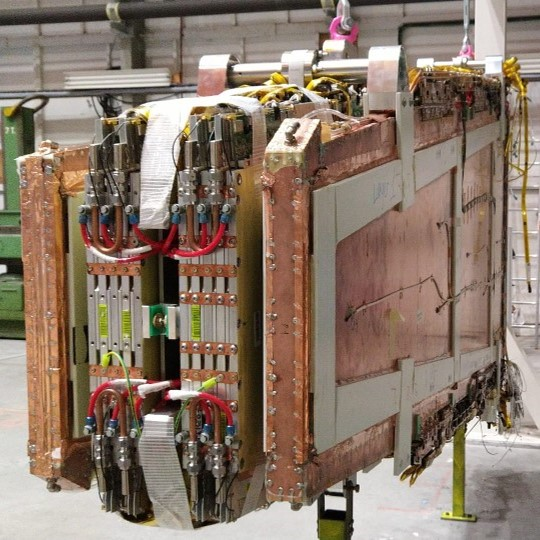
\includegraphics[width=0.35\textwidth]{figures/sector.jpg}
  \caption{Left: An sTGC wedge. The white frame outlines the individual quadruplet modules. Right: A completed sector, with two sTGC wedges on the outside and two MM wedges on the inside.}
  \label{fig:wedge_and_sector}
\end{subfigure}

\smallskip

\begin{subfigure}{\textwidth}
  \centering
  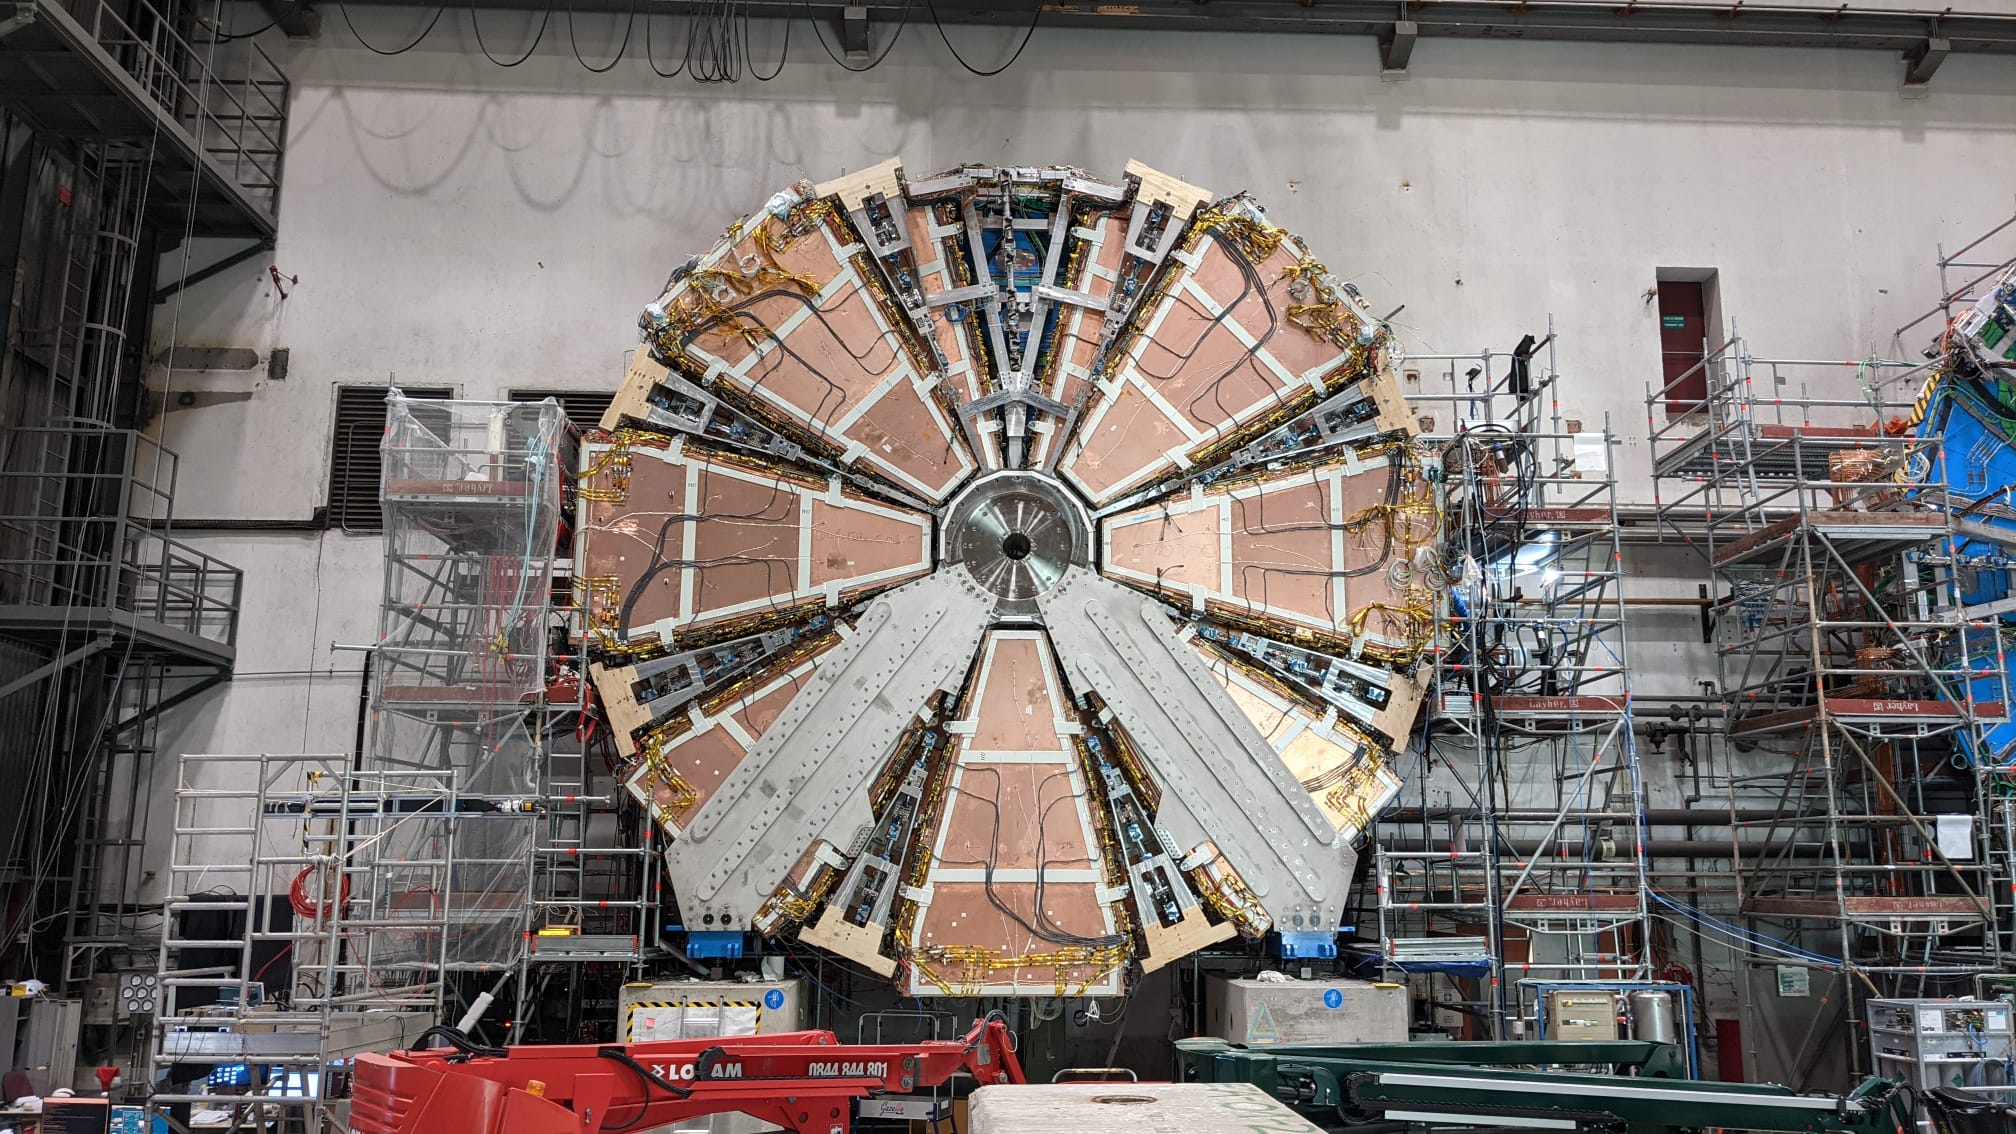
\includegraphics[width=0.7\textwidth]{figures/nsw_2021-05-27_landscape.jpeg}
  \caption{The new small wheel. All sectors except one large sector at the top are installed, revealing two of the smaller sectors that are normally hidden under the large sectors and support bars. The NSWs are \SI{10}{m} in diameter. }
  \label{fig:nsw}
  \end{subfigure}
\caption{Images breaking down some of the construction units of the NSWs.}
\label{fig:nsw_breakdown}
\end{figure}
\newpage
\restoregeometry
% For the tracking and triggering goals, each chamber must have a position resolution of $\sim$\SI{100}{\micro\meter}. 

%TODO : Pivot vs confirm? You don't mention the difference anywhere.

% --------------------------------------------------
\section{Micromegas}
% --------------------------------------------------

Micromegas have three components: a drift plane, a gas gap, a mesh, and readout strips, as shown in figure~\ref{fig:micromega}. High voltage is applied to the readout strips. An ionization event in the gas causes electrons to drift towards the mesh. Once they arrived, they are amplified by the strong field and the avalanche is picked up by the readout electrodes. The small distance between the readout electrodes and the mesh, \SI{128}{\micro\meter}, means that positive ions are evacuated in $\sim$\SI{100}{\nano\second}, making micromegas a good choice for high rate environments~\cite{nsw_tdr}. The small pitch of the readout electrodes, \SI{0.425}{mm}, provides spatial resolution much better than \SI{100}{\micro\meter}~\cite{stelzer_new_2016}. MM quadruplets will be used for offline precision tracking~\cite{nsw_tdr}.

\begin{figure}
    \centering
    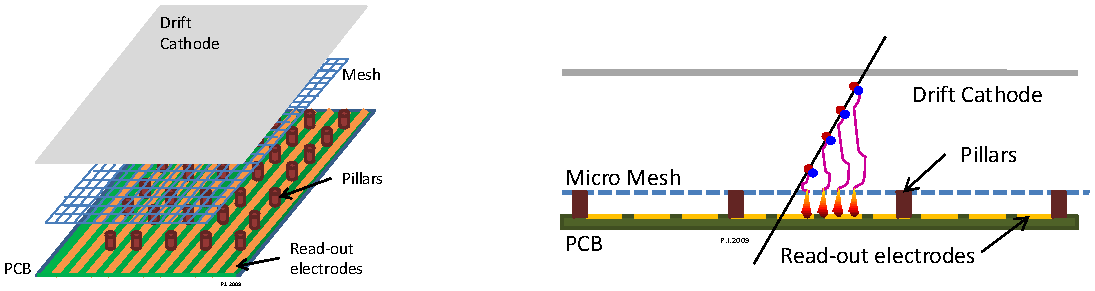
\includegraphics[width = 0.9\textwidth]{figures/micromegas.png}
    \caption{Sketch the micromega operating principle. Positive high voltage is applied to the readout electrodes, which creates a strong field between the mesh and the readout electrodes, and a weaker field between the mesh and the drift cathode. Amplification takes place between the readout electrodes and the mesh. Figure from~\cite{nsw_tdr}}
    \label{fig:micromega}
\end{figure}

% --------------------------------------------------
\section{Small-strip thin gap chambers}
% --------------------------------------------------

\begin{figure}
    \centering
    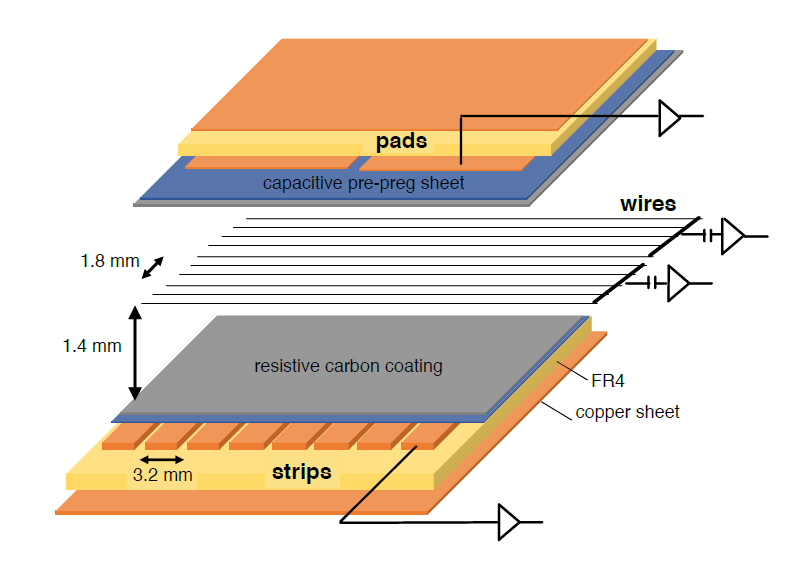
\includegraphics[width = 0.9\textwidth]{figures/stgc_internals.png}
    \caption{Interal structure of an sTGC, zoomed into the area under approximately 1 pad. High voltage is applied to wires suspended in the gas volume to create an electric field. A passing muon causes an ionization avalache that is picked up by the wire, strip and pad electrodes~\cite{lefebvre_precision_2020}.}
    \label{fig:stgc_internals}
\end{figure}

sTGCs are gas ionization chambers operated with a CO$_2$:n-pentane ratio of 55:45. Gold-plated tungsten wires, \SI{50}{\micro\meter} in diameter and with \SI{1.8}{mm} pitch, are suspended between two cathode planes made of FR-4, each \SI{1.4}{mm} away. One cathode board is segmented into pads of varying area (around \SI{300}{cm^2} each), and the other segmented into strips of \SI{3.2}{mm} pitch, perpendicular to the wires. High voltage is applied to the wires and the cathode planes are grounded~\cite{nsw_tdr, perez-codina_small-strip_2016}. When a muon passes through, the gas is ionized and the electric field in the gas gap causes an ionization avalanche~\cite{townsend_electricity_1915}. The motion of the ions and electrons are picked up on the nearby wire, strip and pad electrodes. The hatching of the strips and wires establishes a coordinate system from which to extract the coordinate of the muon as it passes through the layer. The graphite coating resistivity and the capacitance between the strips and pads have been tuned to optimize the rate capability. 

A 3-out-of-4 coincidence in the pad electrodes of a quadruplet will define a region of interest where the strip and wire electrodes should be readout. Then, a track segment with the required angular resolution can be constructed and provided as input to the L1 trigger~\cite{nsw_tdr}. For the next run of ATLAS (run-3), the L1 trigger will pass if the track segment from the small wheel matches a region of interest defined by the TGCs of the big wheel~\cite{tdaq_phase1_tdr, nsw_tdr}. The increased angular resolution and $\eta$ coverage of the quadruplets will be an improvement in the triggering scheme over the current SW TGCs~\cite{nsw_tdr}. After the phase-II upgrade of the trigger and data acquisition system scheduled for $\sim$2025, which includes upgrades to the big wheel's angular resolution, there will only be a trigger if the combined track points back to the interaction point, increasing the muon $p_T$ resolution~\cite{nsw_tdr, tdaq_phase2_tdr}. 

Signal is readout from groups of successive wires, so the position resolution in the direction perpendicular to the wires is $\sim$\SI{10}{mm}. The resolution in this direction does not matter since it will give the symmetric azimuthal coordinate in ATLAS. Good resolution on the $\eta$ coordinate, perpendicular to the strips, is important~\cite{nsw_tdr}. The average single chamber position resolution in the strip coordinate was \SI{45}{\micro\meter} for perpendicular muon tracks as measured in a test beam~\cite{abusleme_performance_2016}~--- well within design specifications. When four sTGCs are glued together into a quadruplet the design angular resolution of \SI{1}{mrad} in the strip coordinate is achievable~\cite{nsw_tdr, perez-codina_small-strip_2016}. 

Therefore, sTGCs are able to meet the precision tracking and triggering goals they were designed for. To ensure they can deliver once installed in ATLAS, knowing the position of the strips to within their position resolution in the ATLAS coordinate system is necessary. The NSW alignment system, detailed in section~\ref{sec:nsw_alignment} monitors the position of alignment platforms installed on the surface of the wedges. The alignment platforms are installed with respect to an external reference on the sTGCs: two brass inserts on each strip layer on one of the angled sides of each quadruplet (shown in figure~\ref{fig:brasses}). So the challenge of positioning the strips in ATLAS can be separated into two steps: first, position the strips with respect to the brass inserts; second use the alignment system to position the alignment platforms. The next section provides some pertinent details on the sTGC construction process, with steps that affect the position of the strips highlighted.
% The position of the strips can be separated into two stages. First, the NSW alignment system monitors the position of alignment platforms installed on the surface of the wedges, as detailed in section~\ref{nsw_alignment}. Second, the internal geometry of the chambers must be referenced with respect to the wedges. Parts of the sTGC construction process that affect the position of the strips are explained in section~\ref{sec:stgc_construction}. The chapter closes 

\begin{figure}
\centering
\begin{subfigure}{.5\textwidth}
  \centering
  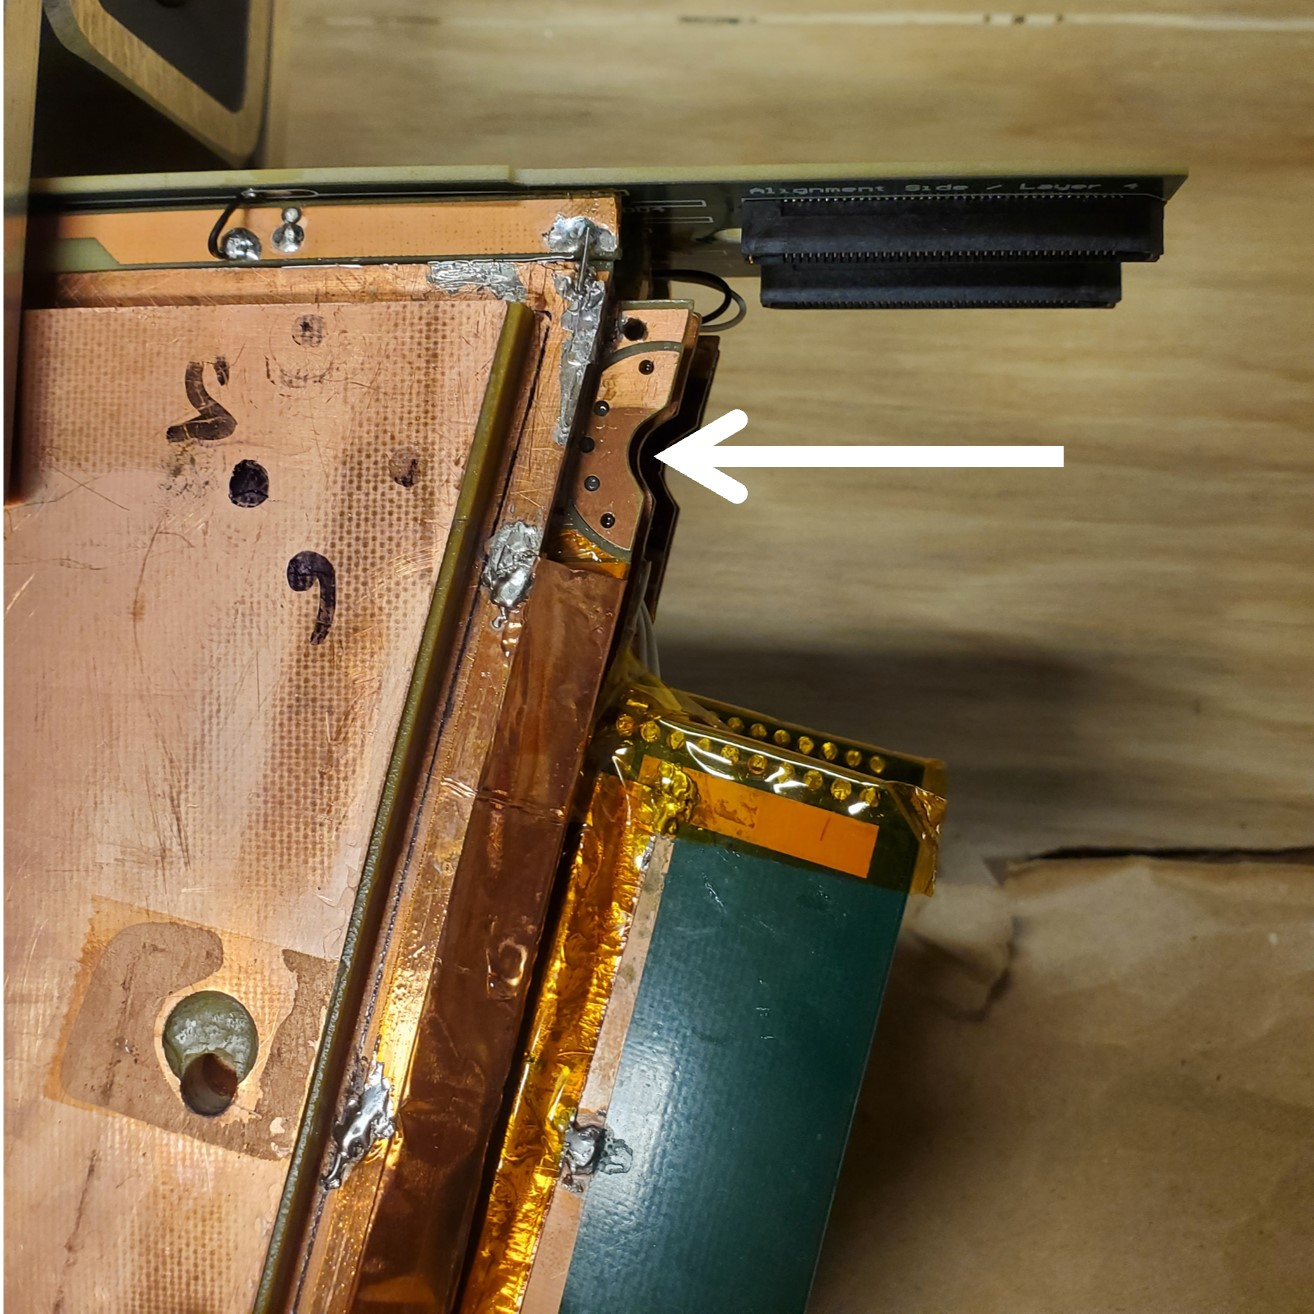
\includegraphics[width=\linewidth]{figures/brass_top.jpg}
  \caption{Brass insert near long edge.}
  \label{fig:brass_top}
\end{subfigure}%
\begin{subfigure}{.5\textwidth}
  \centering
  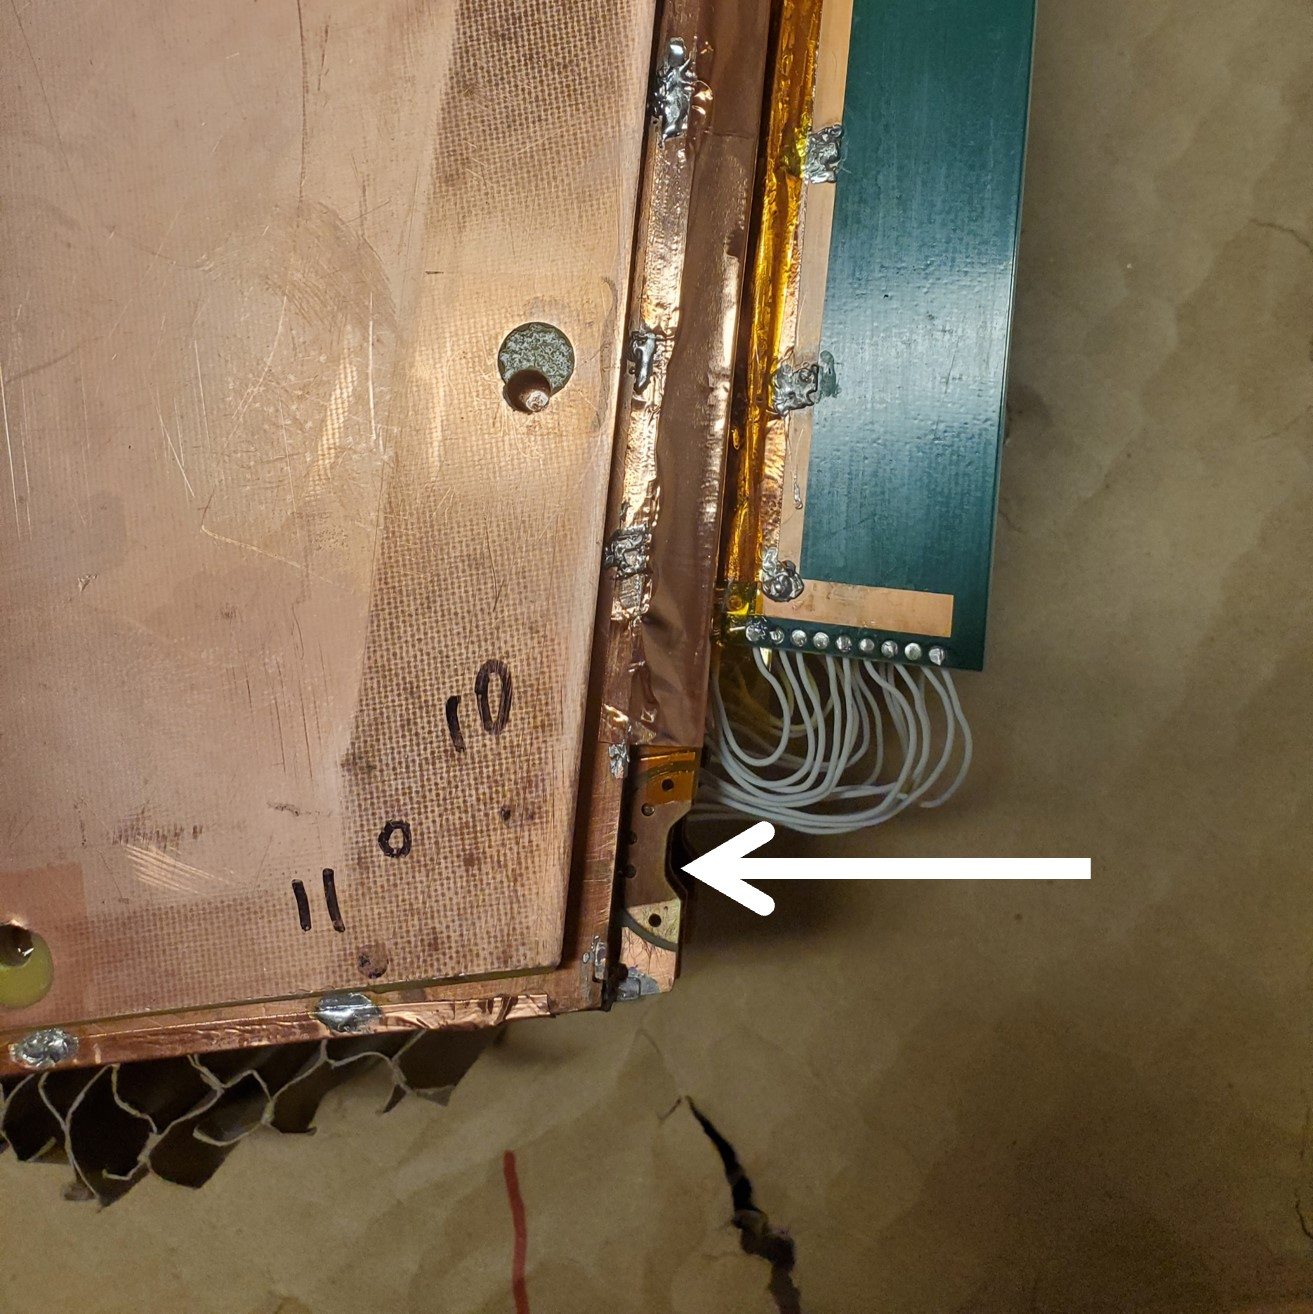
\includegraphics[width=\linewidth]{figures/brass_bottom.jpg}
  \caption{Brass insert near short edge.}
  \label{fig:brass_bottom}
\end{subfigure}
\caption{The brass inserts sticking out from the gas volumes of an sTGC quadruplet. These inserts were pressed against alignment pins when the individual sTGCs were being glued together.}
\label{fig:brasses}
\end{figure}

% However, the accuracy of the hit positions on each layer depends on how well the position of the strips are known in the ATLAS coordinate system. 

% Each strip cathode board has two brass inserts, one near the long edge and one near the short edge, pictured in figure~\ref{fig:brasses}. The inserts were used to align the strip layers of a quadruplet during construction. They were supposed to control the position of the strips to within \SI{40}{\micro\meter} within nominal. The idea was that the NSW alignment system would monitor the position of points on the surface of an sTGC wedge (discussed in section~\ref{sec:nsw_alignment}) and that the combined external and internal alignment uncertainty on the strip positions would be acceptably small for the precision tracking goals~\cite{nsw_tdr}. Uncontrolled offsets of strip positions on an sTGC layer will bias the reconstructed hit position and hence the track, reducing accuracy of the momentum measurement. To understand the source of offsets in strip positions and misalignments between strip layers, pertinent details of the sTGC construction process are presented in the next section.

% In addition, the sTGC quadruplets should be able to provide precision tracking within \SI{100}{\micro\meter} per plane in the event of a MM module failure.

% --------------------------------------------------
\section{sTGC Quadruplet Construction}
% --------------------------------------------------
\label{sec:stgc_construction}

\textcolor{red}{Can I add photos? I found some on the public TRIUMF website of the graphite spraying. Can't find many from Carleton. Where am I allowed to get photos from?}

Five countries were responsible for producing the sTGC modules of varying geometries for the NSW: Canada, Chile, China, Israel and Russia. Canada was responsible for 1/4 of the required sTGCs, of three different quadruplet geometries. The steps of the construction process in each country were similar~\cite{nsw_tdr}. The process followed in Canada is detailed.

TRIUMF in Vancouver, British Columbia was responsible for preparing the cathode boards. The boards were made and the electrodes etched at a commercial laboratory, Triangle Labs, in Carson City, Nevada. Once completed they were sent to TRIUMF to be sprayed with graphite and otherwise prepared~\cite{carlson_results_2019}. The boards are commercial multilayer printed circuit boards, but the strip boards required precision machining to etch the strip pattern~\cite{nsw_tdr}. A coordinate measuring machine (CMM) or FaroArm was used to digitize each strip. Four quality parameters describing non-conformities in the strip pattern of each board were derived from the data and the results are available on a QA/QC database. The parameters and the so-called CMM data is described in full in Carlson's thesis~\cite{carlson_results_2019}. Triangle Labs also machined the two brass inserts into each strip board. Due to time constraints, tolerances on the non-conformities in the etched strip pattern with respect to the brass inserts were loosened, with the condition that the strip positions would have to be corrected for~\cite{carlson_results_2019}. 

The prepared boards were sent to Carleton University in Ottawa, Ontario for construction into sTGCs and quadruplets. First, the wires were wound around the pad cathode boards using a rotating table and the wires soldered into place. Then, a wound pad cathode board was held by vacuum on a granite table, flat to within \SI{20}{\micro\meter} and a strip cathode board glued on top to create an sTGC. Holding one sTGC flat with the vacuum, another was glued on top to create a doublet, then two doublets were glued together to create a quadruplet. When gluing sTGCs together, the brass inserts were pushed against alignment pins with the goal of keeping the strip layers aligned within tolerance. However, non-conformities in the shape of the brass inserts and the position of the alignment pins resulted in misalignments between the brass inserts and strips on successive layers. Precise alignment of the pad boards or wires with respect to the strip boards did not have to be so tightly controlled because pads do not measure the precision coordinate. 

The Carleton team finished the quadruplets by installing adaptor boards on the angled sides that allow front end electronics to be attached to each layer to readout the electrodes. Completed quadruplets were sent to McGill University where they were characterized with cosmic rays. The details of cosmic ray testing are described in chapter~\ref{chap:cosmics}. Quadruplets were then sent to CERN where they were assembled into wedges and alignment platforms installed. The alignment platforms were installed using a jig positioned with respect to the brass inserts. Completed wedges were assembled into sectors then installed on the NSWs.

% So, during cathode board construction the etched strip pattern could be shifted off of nominal with respect to the brass inserts. While gluing sTGCs together, non-conformities in the shapes of the brasses and the position of the alignment pins resulted in misalignments between the brass inserts that mean they are not a uniform reference for every layer of the quadruplet. 

The board construction process had two steps where strip positions could be shifted off of nominal. First, there could be non-conformities in the etched strip pattern, described by the four quality parameters~\cite{carlson_results_2019}. Second, non-conformities in the shape of the brass inserts and in the position of the alignment pins resulted in misalignments between strips on different layers. The result was that the brass inserts were not a reliable reference point and strips can be offset from their design position by up to hundreds of micrometers. Offsets in strip positions from nominal in Canadian quadruplets were shown to be random~\cite{carlson_results_2019}, so no one correction would suffice. The offsets must be measured and corrected for in the ATLAS offline software, \package{Athena}, which is responsible for precision tracking. Understanding the work ongoing to make measurements of offsets and correct for them requires understanding the main strategy used by the NSW alignment system.

% Two sources of misalignment resulted at board level: non-conformities in the placement and shape of the brass inserts and non-conformities in the strip pattern. Carlson addressed the non-conformities in the strip pattern of Canadian cathode boards in his thesis~\cite{carlson_results_2019}. A coordinate measuring machine (CMM) or FaroArm was used to digitize the etched strip pattern of each board. Four quality parameters describing non-conformities in the strip pattern were derived from the data and the results are available on a QA/QC database. The parameters were offset, angle (rotation), scale and non-parallelism, defined in ful in Carlson' thesis. Often, alignment models only consider an offset and rotation. 

% Once the cathode boards were prepared, they were sent to TRIUMF in Vancouver, British Columbia to be sprayed with the graphite coating. After spraying, the coating was polished until the resistivity was between 90 and \SI{110}{\kilo\ohm}$/\msquare$, then wire support structures and frames were installed~\cite{nsw_tdr}. The completed boards were sent to Carleton university for construction into gas gaps and multiplets.

% First, anode wires were wound onto the the pad cathode boards using a rotating vacuum table. Then, a pad and strip cathode board has to be glued together to create an sTGC, two sTGCs glued together to create a doublet, and two doublets glued together to create a quadruplet. Gluing was done by holding one side of a cathode board in place with vacuum on a granite table, flat to within \SI{20}{\micro\meter}. A honey comb spacer separates each sTGC layer of a quadruplet. When closing a gas gap, micrometer misalignments between the strip and pad cathode boards do not matter since the pads do not measure precision coordinates. When gluing sTGCs into doublets however, alignment between strip layers had to be controlled by pushing the two brass inserts against alignment pins~--- similarly for gluing together doublets. Once a quadruplet was assembled, adapator boards used to route the electrodes' signals to the front end electronics were soldered on to the angled sides of the quadruplet~\cite{nsw_tdr}. 

% If you want to include the x-ray survery of the brass positions and the microscope method
% At every stage in the process quality control checks were in place for gas, high voltage, and alignment. For alignment, \textcolor{red}{the position of the brasses were recorded in 3D using an x-ray gun~\cite{nsw_tdr} \textit{--> Did this actually happen?}}~\cite{nsw_tdr} and alignment between strips visible outside a quadruplet was checked with a microscope~\cite{carlson_results_2019}. 

% Quality control tests of alignment, ability to hold high voltage, gas sealing etc. were undertaken at every stage in the construction process~-- details can be found in~\cite{nsw_tdr}. The final set of quality control checks and characterization was done at McGill University in Montreal, Quebec. Completed quadruplets were tested for gas leaks, noise and characterized with cosmic rays. The details of cosmic ray testing are described in chapter~\ref{chap:cosmics}.

% Once the quadruplets have been tested with cosmics rays, they are sent to CERN to be further tested, assembled into wedges then sectors, then installed on the NSWs. At the time of writing, all sectors have been installed on both wheels. The first NSW has been lowered into the ATLAS cavern and is being commissioned. The second is scheduled for installation in October, 2021.

% --------------------------------------------------
\section{NSW alignment}
% --------------------------------------------------
\label{sec:nsw_alignment}
%TODO : Mention Athena
% The idea of the NSW alignment system is presented in~\cite{nsw_tdr}, but the details have only been presented internally so far. The original goal of the alignment system was to provide the position with respect to one another of any three chambers traversable by a muon track with an accuracy of \SI{40}{\micro\meter} in the precision coordinate~\cite{nsw_tdr}. Likely for sTGCs, this will mean inputing the strip postions, or parameters to calculate the strip positions, into the ATLAS experiment's offline software, \package{Athena}.

%TODO : 
\textcolor{red}{What figures can I use to show the bars, the alignment jig, the platforms and the optical fibres?}.

The idea of the NSW alignment system is presented in~\cite{nsw_tdr}, but the details have only been presented internally so far. After the wedges are constructed, alignment platforms are installed on every sTGC quadruplet and optical fibres routed to them. Light from the optical fibres will be monitored in real time by cameras (BCAMs) mounted on the alignment bars of the NSWs. The system will thus record the positions of the alignment platforms in the ATLAS coordinate system, accessible at any point during operation \textcolor{red}{Camila Pazos, 2021-02-01 and Chris Armstrong 2021-02-02 during muon week https://indico.cern.ch/event/983500/}. % The final link in the sTGC alignment system requires knowing the position of the strips inside a chamber with respect to the alignment platforms.

% If you want to mention the alignment jig in the last paragraph:
% They are positioned with the help of an alignment jig, which is like a frame that can be positioned on top of a wedge with cut outs indicating the correct position for the alignment platforms. The jig is positioned with respect to the brass inserts \textcolor{red}{[Benoit 2020-01-20, 2020-04-16 presentations]}.

% The goal was to control the position of the strips in the chamber to within ~\SI{40}{\micro\meter} for precision tracking goals~\cite{nsw_tdr} --- then knowing the position of the brass inserts with respect to the alignment platforms would allow the strips to be positioned accurately enough. That is the alignment scheme shown in solid arrows in figure~\ref{fig:alignment_elements}. Due to time constraints, tolerances on the non-conformities in the etched strip pattern were loosened, with the condition that the strips positions would have to be corrected for in the software~\cite{carlson_results_2019}. Then, non-conformities in the brass inserts, misalignment of the pins the brass inserts were pushed against, and shifts of the strip layers while the glue was curing resulted in misalignments between the brass inserts~-- and between the strips layers ~-- that prevent using the brasses as an external reference of the position of the strips. The misalignments between Canadian sTGCs were shown to be random~\cite{carlson_results_2019}, so no one correction would suffice.

% The original alignment scheme was to use the brass inserts as a reference between the alignment platforms and the individual strips, as shown in the solid arrows in figure~\ref{fig:alignment_elements}. \textcolor{red}{Due to time constraints, tolerances on the non-conformities in the etched strip pattern with respect to the brass inserts were loosened, with the condition that the strips positions would have to be corrected for. Corrections will happen in ATLAS offline software, \package{Athena}, that will do the precision tracking~\cite{carlson_results_2019}. --> MOVE THIS} Moreover, non-conformities in the shape of the brass inserts and the alignment pins added misalignment between the inserts of different layers~-- and between the strips of different layers~-- that prevent using the brass inserts as a reference. Offsets in strip positions from nominal in Canadian quadruplets were shown to be random~\cite{carlson_results_2019}, so no one correction would suffice.
%TODO : Did other construction sites have this problem?

\begin{figure}
    \centering
    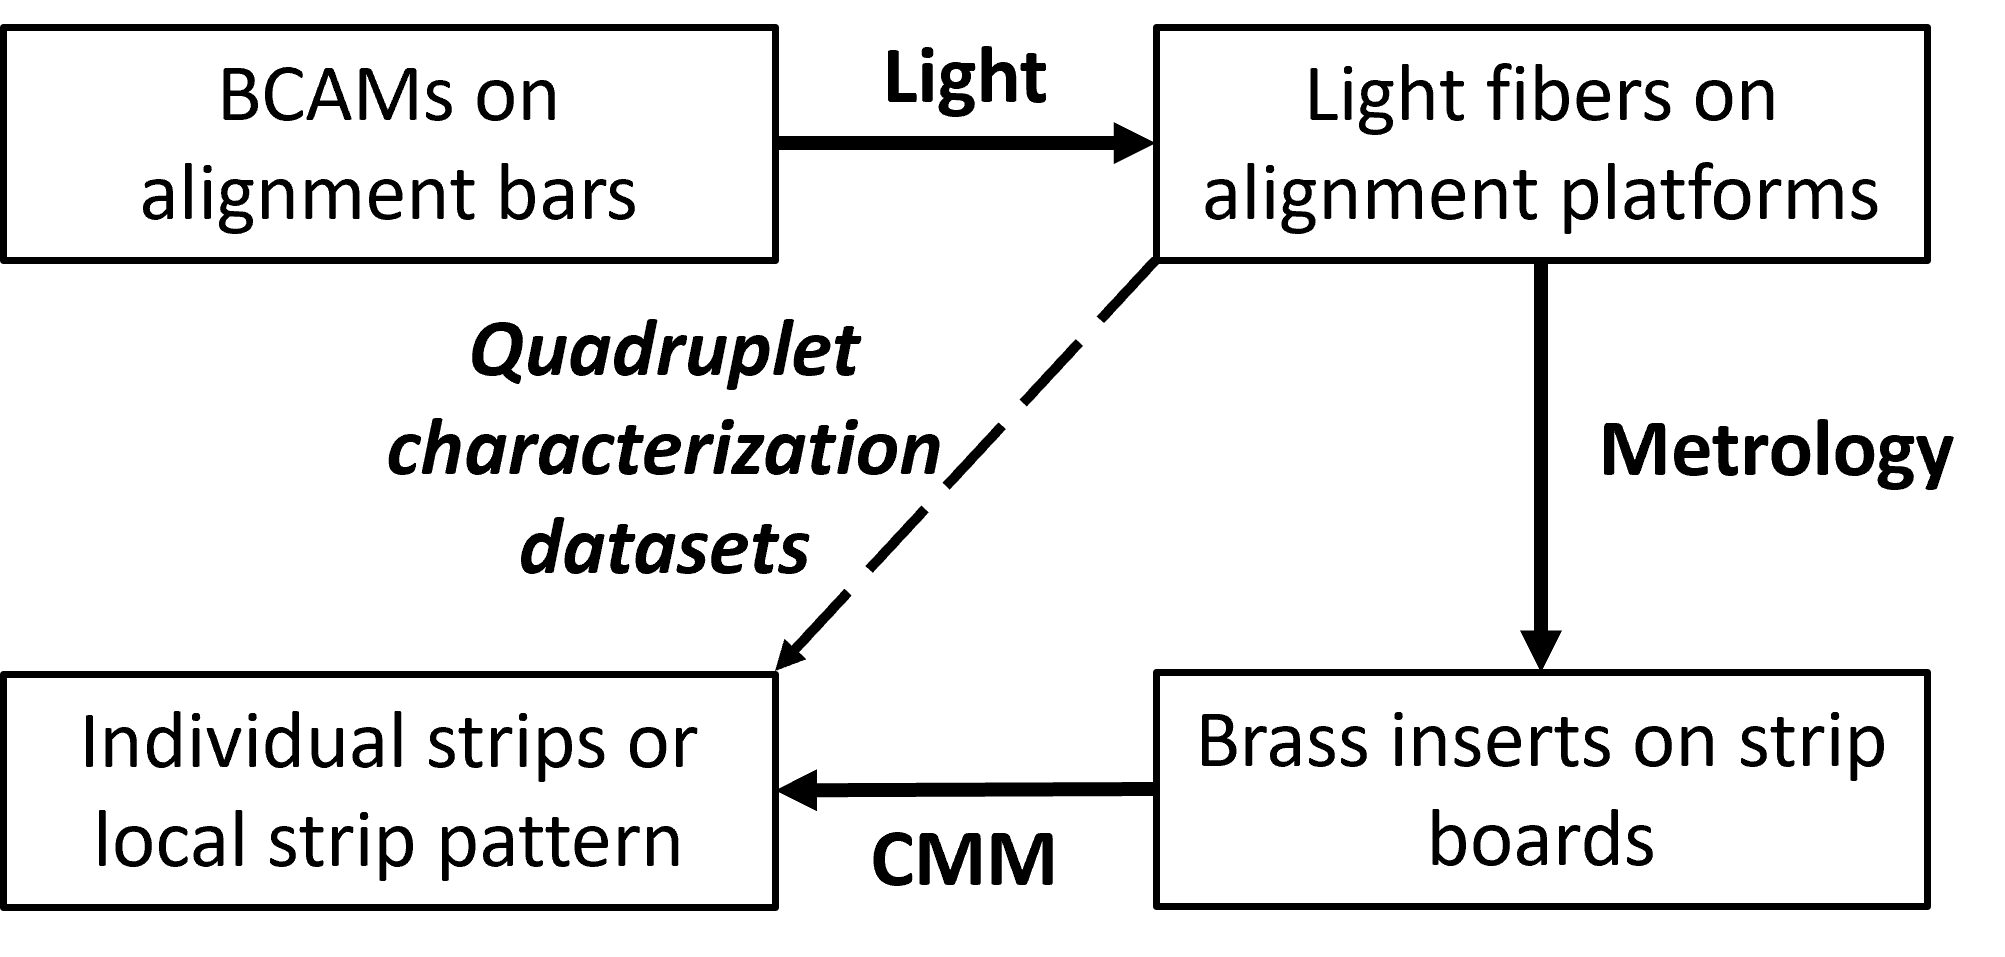
\includegraphics[width = 0.9\textwidth]{figures/alignment_system_element_relations.png}
    \caption{How the different elements of the sTGC alignment system relate to one another. The solid arrows denote the planned alignment scheme. The dashed arrow shows the modification being finalized now. This figure is based off of \textcolor{red}{Benoit's presentation, 2021-01-30.}}
    \label{fig:alignment_elements}
\end{figure}

The original alignment scheme was to use the brass inserts as a reference between the alignment platforms and the individual strips, as shown in the solid arrows in figure~\ref{fig:alignment_elements}, which will no longer work. The position of the alignment platforms will still be known in ATLAS thanks to the alignment system, so a different method to get the position of the individual strips with respect to the alignment platform is currently in its final stages. It uses the yet-unmentioned x-ray dataset to calculate offsets of the strip pattern of an sTGC layer in a local area (local offset) with respect to the alignment platforms directly. Effectively, the reference to the brass inserts is skipped, represented as the dashed line in figure~\ref{fig:alignment_elements}. The goal of this thesis is to validate the x-ray local strip pattern offsets with cosmic muon data. In chapter~\ref{chap:cosmics}, how cosmic muon data collection and processing is done at McGill University is presented. Chapter~\ref{chap:cosmics_for_positioning} and \ref{chap:xray}detail how measurements of local strip pattern offsets are measured with cosmic muon data and x-ray data. In chapter~\ref{chap:comparison}, cosmic muon and x-ray local strip pattern offsets are compared to validate the x-ray dataset. Finally, in chapter~\ref{chap:outlook}, the context of these results in the alignment scheme is presented.

% Snippets
%The main dataset was collected using x-rays as the probe. The x-ray data has been combined with the CMM data to create an alignment model that can be used to estimate the position of each strip. The goal of this work was to validate the measurements of strip pattern offsets done with the x-ray dataset with the cosmic muon data. Currently, only modules made in Canada have been analyzed in this way, but the method applies for other countries that were able to collect cosmic muon data on multiple quadruplet layers. 

%Moreover, as-built alignment parameters must be measured and extracted to ensure proper function and provide a way to correct for misalignment. The next section breaks down the sTGC construction process to highlight the stages of alignment.
%All countries successfully finished delivering their modules this year, and the sectors have been installed on the NSWs. 































% ==================================================
% CHAPTER 4: Using cosmic muons to measure relative strip position offsets %
% ==================================================

\chapter{Using cosmic muons to measure relative strip position offsets}
\label{chap:cosmics}
% Edit count: Lia - 0, Brigitte - 0

At McGill, among other quality and functionality tests, each Canadian-made quadruplet was characterized with cosmic muons. In this chapter, the cosmic muon experimental setup and how the data was analyzed to provide relative strip position offsets is presented. The analysis method was motivated by the how it could be compared to data collected with the x-ray method, as presented in chapter~\ref{chap:xray}, but also stands alone as a characterization of the alignment between strips of different layers.

% --------------------------------------------------
\section{Experimental setup}
% --------------------------------------------------

Cosmic muon characterization was done with a hodoscope, a complete description of which can be found in~\cite{lefebvre_thesis}.  The quadruplet was placed in the center of the test bench. Above and below it was a layer of scintillator-PMT arrays, labeled in figure~\ref{fig:hodoscope}. When a cosmic muon passed within the acceptance of the hodoscope, at least one scintillator from the top array and at least one from the bottom array fired in coincidence and the coincident signal was used to trigger the readout of the quadruplet's electrodes. The trigger was passed \iffalse through a KC705\footnote{Xilinx, Xilinx Kintex-7 FPGA KC705 Evaluation Kit, EK-K7-KC705-G, 2018} which sent it \fi to the front end boards (FEBs) attached to the adaptor boards of each layer of the quadruplet.

\begin{figure}
    \centering
    \includegraphics[width = 0.9\textwidth]{figures/figure_test_bench.png}
    \caption{Cosmic muon hodoscope at McGill University with sTGC quadruplet in the test bench.}
    \label{fig:hodoscope}
\end{figure}

Operating the chambers also required gas and high voltage. A pentane-CO$_{2}$ mixture was mixed and delivered to each sTGC with a gas system designed and made at McGill University. The gas system was controlled by a slow control program, also made in-laboratory~\cite{keyes_development_2017}. To prepare the quadruplets for operation, CO$_{2}$ was flushed through them overnight. Then, five gas volumes of the pentane-CO$_{2}$ mixture was flushed through (approximately 3 hours). High voltage was provided by CAEN boards. 

% About 2.9 kV vs 3.1 kV
%Although the chambers will be operated at 2.8~kV in ATLAS, the earlier version of the FEBs used at McGill had a worse signal-to-noise ratio for pads, which was compensated for operating the chambers at 3.1~kV, which increased the chambers' gain. Operating at 2.9~kV was sufficient for strip and wire signals and closer to the nominal voltage. Collecting 1 million triggers at each voltage provided enough statistics to calculate characterization metrics, which meant collecting data for just over two hours per quadruplet per voltage.

% --------------------------------------------------
\section{Data acquisition}
% --------------------------------------------------
% It would be great to have a scope trace here, preferably of a strip. Oops.
Each sTGC electrode was connected to a channel on a prototype ASIC\footnote{the VMM3~\cite{iakovidis_vmm3_2017}, designed for the MM and sTGCs of the NSW} on the FEB, attached to the adaptor boards on each layer of a quadruplet.  The ASIC amplified the signal was set to measure and record the signal peak amplitude from electrodes. For each trigger, the signal peak amplitude of all channels above threshold were recorded as an event and stored in a binary file. Thresholds were estimated~\cite{chen_calibration_2019} and adjusted manually in the configuration/readout software before the start of data acquisition. There was an exception to the threshold rule: the signals on strips adjacent to a strip above threshold were also readout using the so-called "neighbour triggering" function of the ASIC. 

The quadruplets were held at 3.1~kV for approximately 2 hours to collect data from 1 million muon triggers.

% --------------------------------------------------
\section{Data preparation}
% --------------------------------------------------
Corrupted data was removed while the raw data was being recorded in a binary file. The binary file could be decoded into a usable ROOT tree offline. 

A hit is defined as a signal recorded from a channel that was above threshold or (in the case of strips) neighbour triggered.  In addition to hits from muons, the quadruplets recorded noise from the electronics and $\delta$-rays. Particularly, the edge strips are very noisy, so hits on a layer that include the edge strips are cut. All electrodes have a pedestal, which was

Also, events that only have hits on pad electrodes (no strips or wires) are cut. 

YOU ARE HERE
% --------------------------------------------------
\section{Clustering}
% --------------------------------------------------

Many of the high-level characterization metrics required rebuilding muon tracks. For events passing quality cuts~\cite{lefebvre_tgc_analysis}, the x- and y-coordinates of the ionization avalanche on each layer were extracted from the signal on the wires and strips respectively for each event, as is sketched in figure~\ref{fig:mwpc_coords}. In this work, $x$ was the coordinate perpendicular to the wires and $y$ was the coordinate perpendicular to the strips, as is drawn in figure~\ref{fig:mwpc_coords}.

The x-coordinate was taken as the center of the wire group with the maximum PDO, since the wire groups' pitch (\SI{36}{\milli\meter}) was larger than the typical charge spreading. Assuming that the true x-position of the hit was uniformly distributed over the width of the wire group, the uncertainty in the x-position was given by $\frac{36~mm}{\sqrt{12}} = 10~mm$~\cite{Sauli:117989}.

The y-coordinate was taken as the Gaussian mean of the PDO distribution across groups of contiguous strips. The process of grouping contiguous strips with signal above threshold\footnote{Note that during cosmic ray testing, the hardware was configured to also record the PDO of strips adjacent to a strip above threshold.} was called clustering, and the resulting group was called a cluster. Figure~\ref{fig:mwpc_coords} sketches the clustering process and a sample cluster is shown in figure~\ref{fig:sample_cluster}. Typically, clusters were built of 3-5 strips. The thickness of the graphite coating over the cathode boards determined how many strips picked up the ionization image charge. Larger clusters were more likely caused by $\delta$-rays since they spread the cloud of ionization. 

\begin{figure}
    \centering
    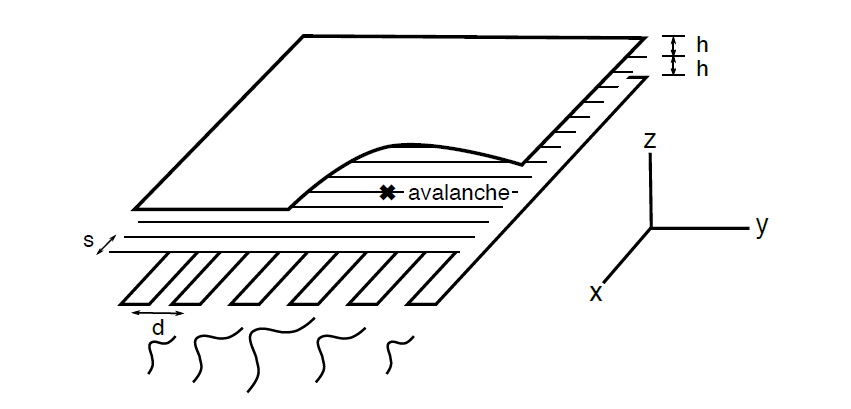
\includegraphics[width = 0.7\textwidth]{figures/mwpc_lefebvre_thesis_gatti.png}
    \caption{A sketch of an sTGC-like detector. The position of the avalanche could be extracted from the wires and strips that picked up the avalanche signal. The signals on individual strips are sketched. Clustering was the processs of fitting a Gaussian to the peak value of the signals on individual contiguous strips, as is done in figure~\ref{fig:sample_cluster}. In this work, the x(y)-coordinate will always refer to the coordinate perpendicular to the wires (strips)~\cite{lefebvre_thesis, gatti_optimum_1979}.}
    \label{fig:mwpc_coords}
%\end{figure}
    \vspace*{\floatsep}
%\begin{figure}
    \centering
    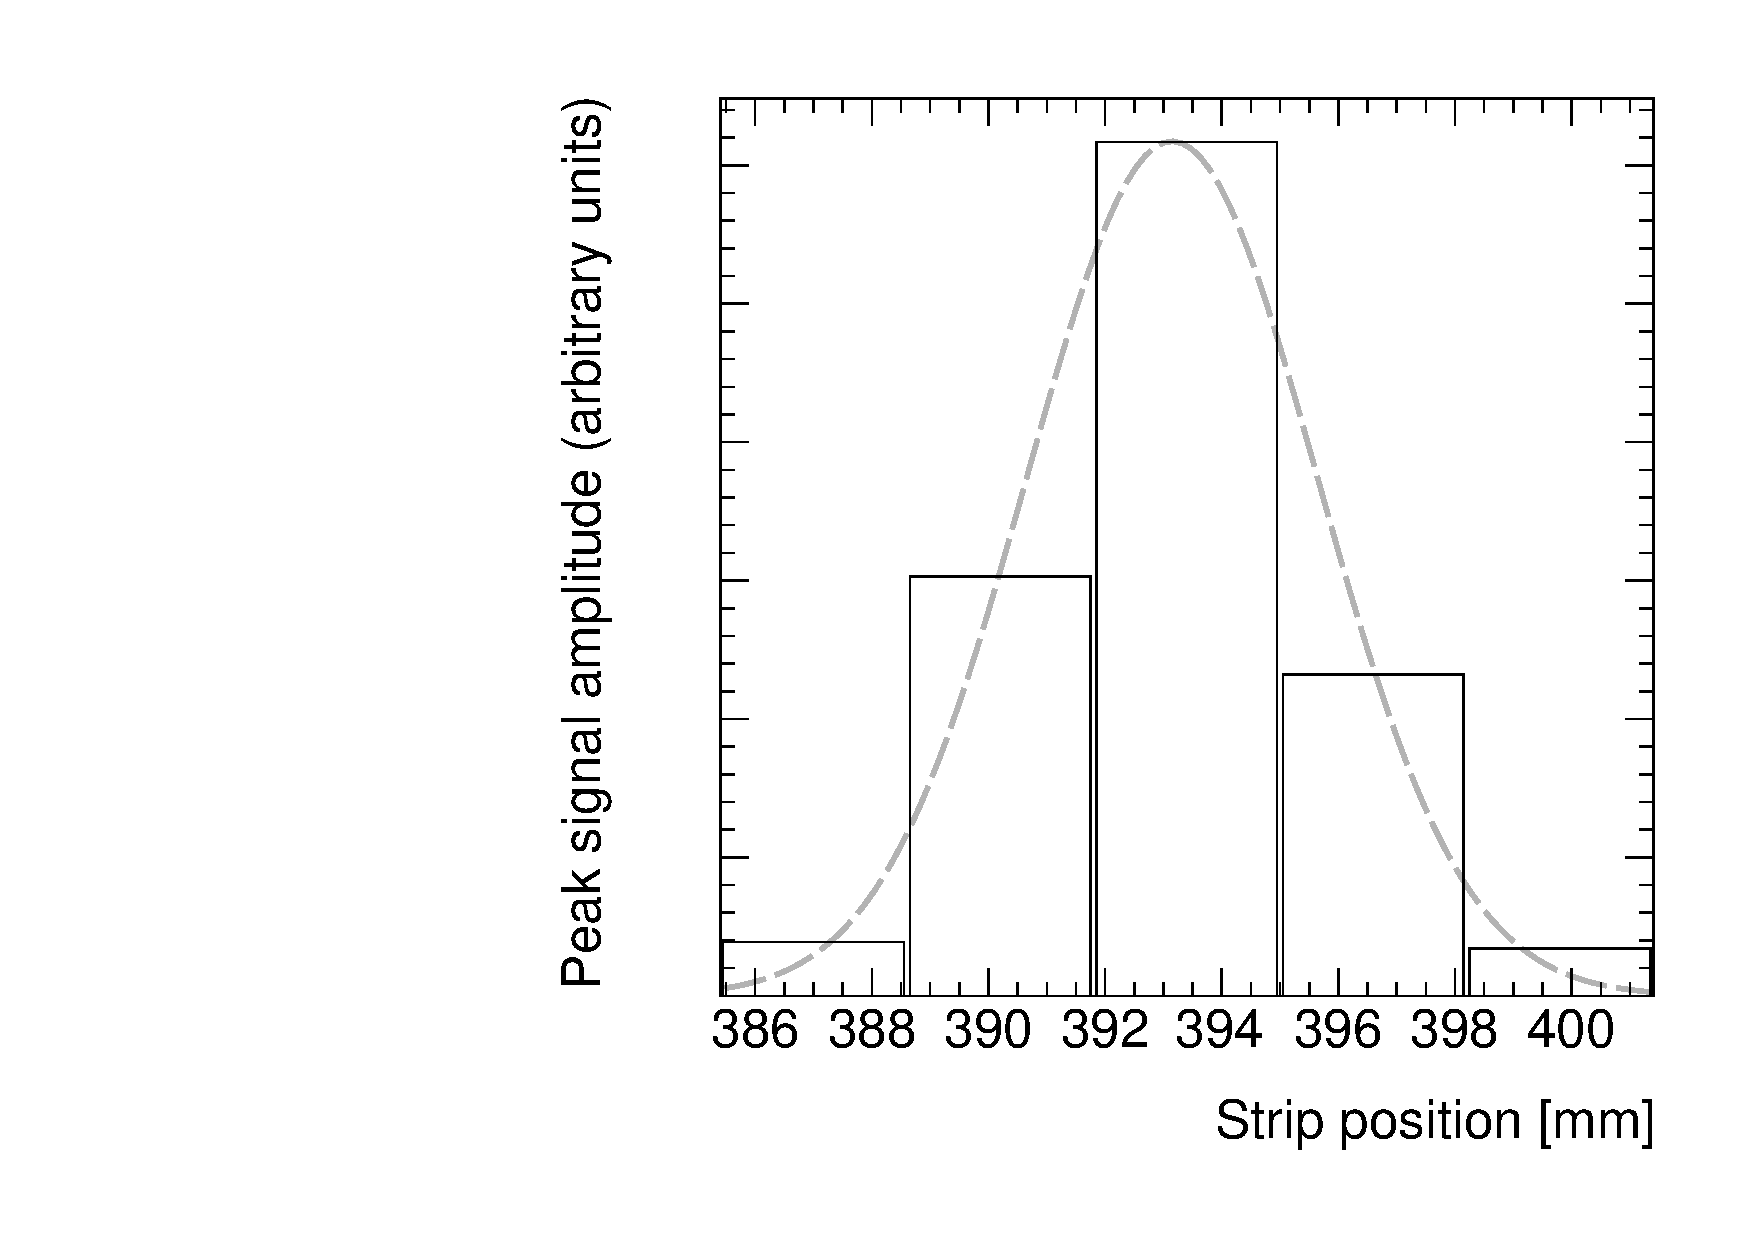
\includegraphics[width = 0.5\textwidth]{figures/sample_cluster_QL2C04_event5_layer2.pdf}
    \caption{A sample cluster resulting from the current picked up on a group of strips (presumably) after the passing of a muon. The grey line is a Gaussian fit.}
    \label{fig:sample_cluster}
\end{figure}

The uncertainty in the y-coordinate could have been taken as the fitted cluster mean's statistical uncertainty; however, after comparing the difference in cluster means for different fitting algorithms in appendix~\ref{sec:appendix_clustering_cluster_fit}, \SI{60}{\micro\meter} of uncertainty was assigned.

The coordinates of the avalanches' on all layers were used to reconstruct tracks in x and y respectively. Most tracks passing quality cuts were probably cosmic muons, but of course some $\delta$-rays and noise contributed. The tracks were then used to calculate characterization metrics like electrode efficiency and spatial resolution, the details of which are discussed in~\cite{lefebvre_thesis}.

%TODO : Figure out the correct citation for quality cuts. Is Benoit's thesis ok or should you just point people to the software? 
%TODO : Should I be citing sections as opposed to the whole thesis? I feel like I'll keep citing different sections of thesis.
%TODO : Include hit and track map? - yes if Brigitte says you need a num_entries plot in chapter 3. You didn't include it because you never mention wire supports in TH2 analysis. But if you want to add num entries for clarity, include cluster map here. Cluster map > raw hits because less cuts and gets across the idea that x is just hit or no hit while y comes from clustering. 

Three methods were used to characterize each quadruplet's alignment: the CMM method, cosmic ray tracing and x-ray profile reconstruction. For present purposes, the CMM method was described sufficiently in the introduction. The x-ray method is detailed in chapter~\ref{chap:xray}. How cosmic ray tracing was used for alignment studies, with the goal of independently validating the x-ray method, is the main focus of this chapter and this thesis. 

% Edit count: Lia - 2, Brigitte - 0
% --------------------------------------------------
\section{Measuring local offsets in strip pattern using cosmics data}
% --------------------------------------------------

Misalignments can be modeled as passive transformations. Ideally, a misalignment model would be chosen and the parameters (for example, a global offset and rotation for each layer) calculated. To understand the potential of cosmic muon data, it is useful to define a local offset. For each area of a strip layer, the local offset is the shift of the strip pattern in that area with respect to the nominal geometry.  Local offsets systematically change the strip that is hit by a muon passing through the area. The \package{tgc\_analysis/CosmicsAnalysis} software assumes the nominal geometry, so the recorded muon y-position ($y$) is shifted opposite to the local offset ($d_{local}$),
% Maybe useful sentence?: The local offset is a result of the non-conformities in the strip pattern etching and inter-layer misalignments.
\begin{equation}
    y = y_{nom} - d_{local},
    \label{eqn:local_translation}
\end{equation}
% Maybe useful sentence?: The true position of individual cosmic muons is not known, and in the analysis the four detector planes float with respect to a software-implemented origin that is not associated with a fixed physical location.
where $y_{nom}$ is the position of the muon that would have been recorded if there was no local offset. Equation~\ref{eqn:local_translation} ignores other factors that could affect the cluster position (like position resolution). The local offset is unknown and there was no external reference to measure $y_{nom}$. Therefore, only relative alignment parameters can be extracted. 

The minimal relative coordinate system uses two reference or fixed layers~\cite{lefebvre_thesis}. The hits on the two fixed layers were used to create tracks that can be interpolated or extrapolated (polated) to the other two layers. The residual of track $i$, $\Delta_i$ is defined as,
\begin{equation}
    \Delta_i = y_{i,hit} - y_{i,track},
    \label{eqn:residual}
\end{equation}

where $y_{i,hit}$ is the recorded hit position and $y_{i,track}$ is the polated track position built from hits on the two reference layers. Track residuals are affected by the local offset in the area of each layer's hit. As an example, in figure~\ref{fig:fake_event_display}, the residual on layer 2 perhaps indicates that layer 2 is offset with respect to layers 1 and 4 in the area of the track. Of course, a single track residual says nothing of the real relative local offset because of the limited spatial resolution of the detectors and fake tracks caused by noise or delta rays. However, the mean of residuals for all tracks in a region will be shifted systematically by the local offsets between layers~\cite{lefebvre_thesis}. For a perfectly aligned quadruplet, the mean of residuals should be zero in all regions and for all reference frames, unlike the example regions in figure~\ref{fig:res_dist}.
\begin{figure}
    \centering
    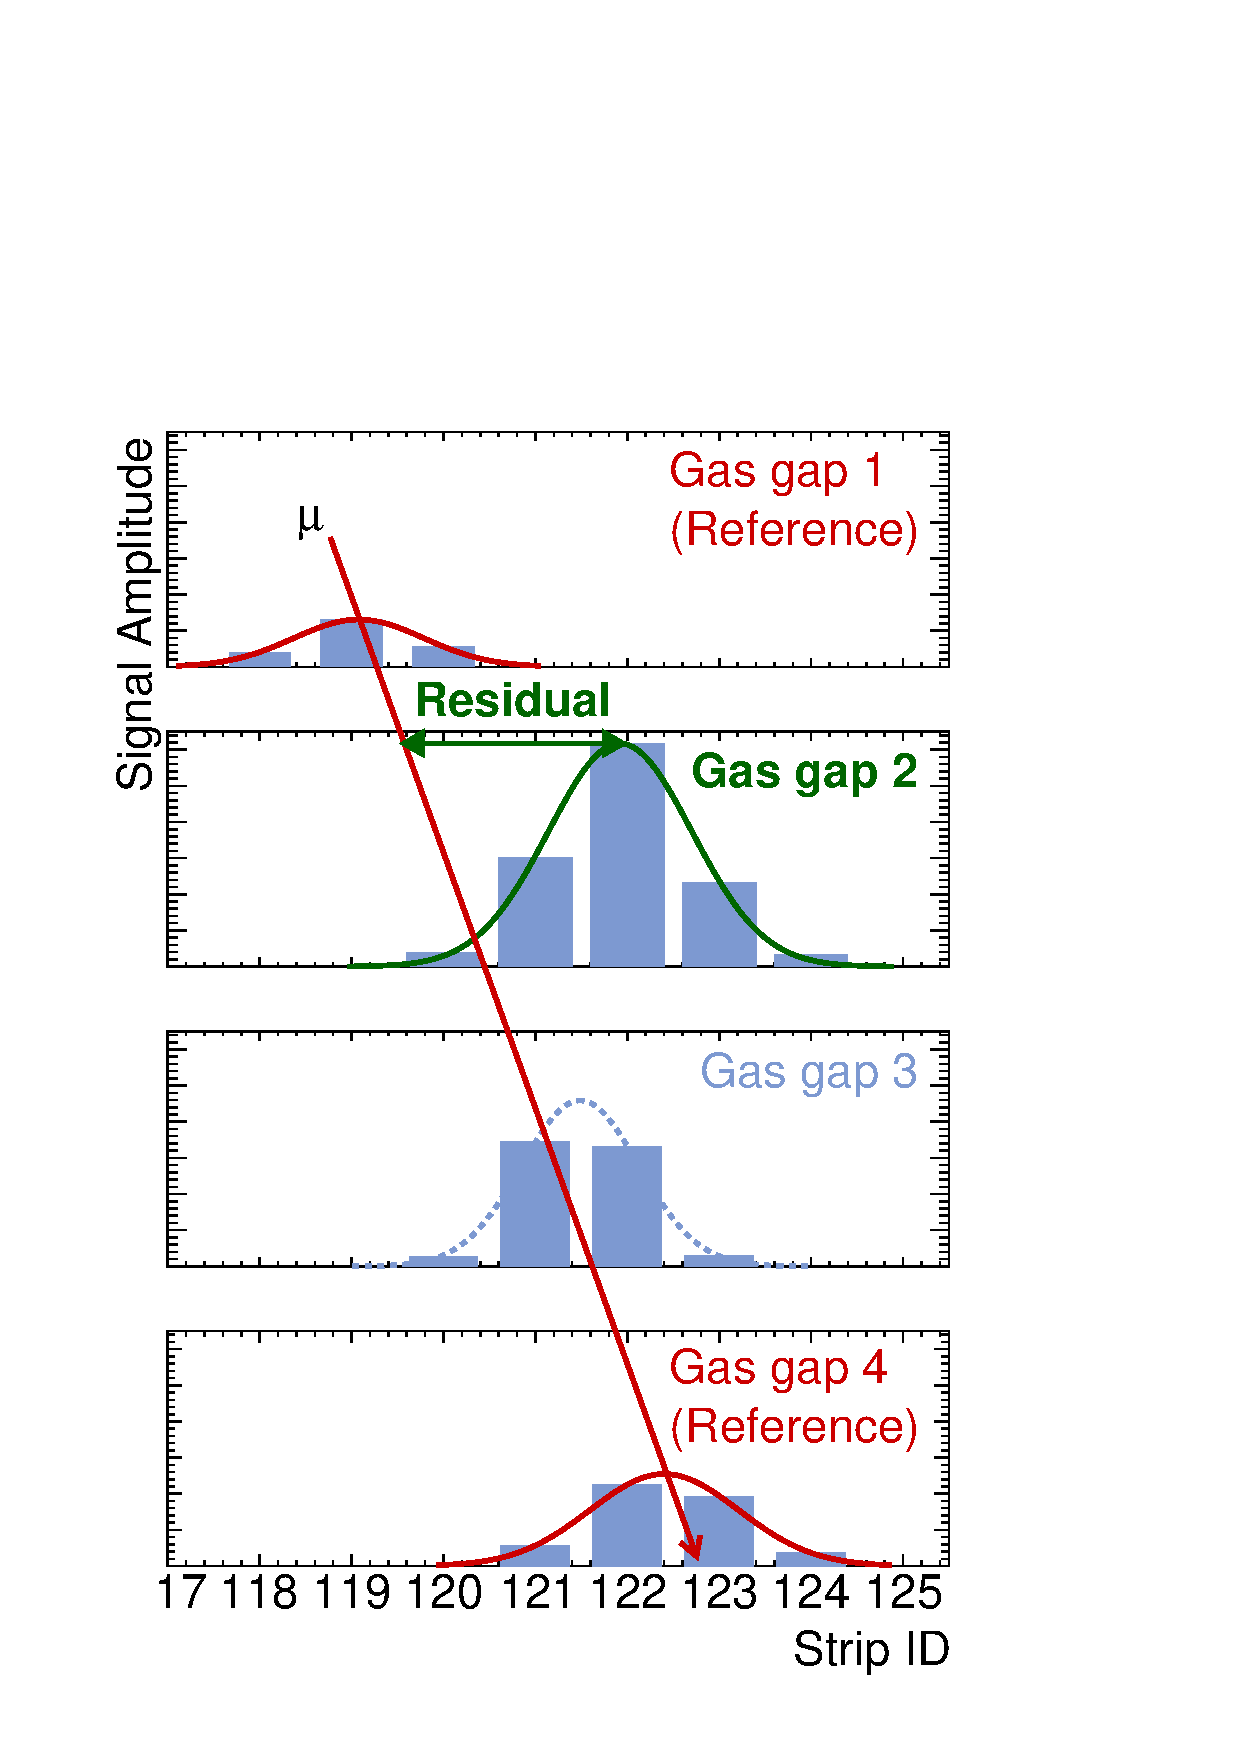
\includegraphics[width = 0.9\textwidth]{figures/figure_fake_event_display.pdf}
    \caption{Representation of a muon event recorded by an sTGC. The clusters are fit with a Gaussian and the mean is taken as the hit position. A track is built from the chosen reference layers, 1 and 4, and the residual calculated on layer 2. The clusters come from a real muon event, but their positions were modified to highlight the residual on layer 2.}
    \label{fig:fake_event_display}
\end{figure}

\begin{figure}
\centering
\begin{subfigure}{.5\textwidth}
  \centering
  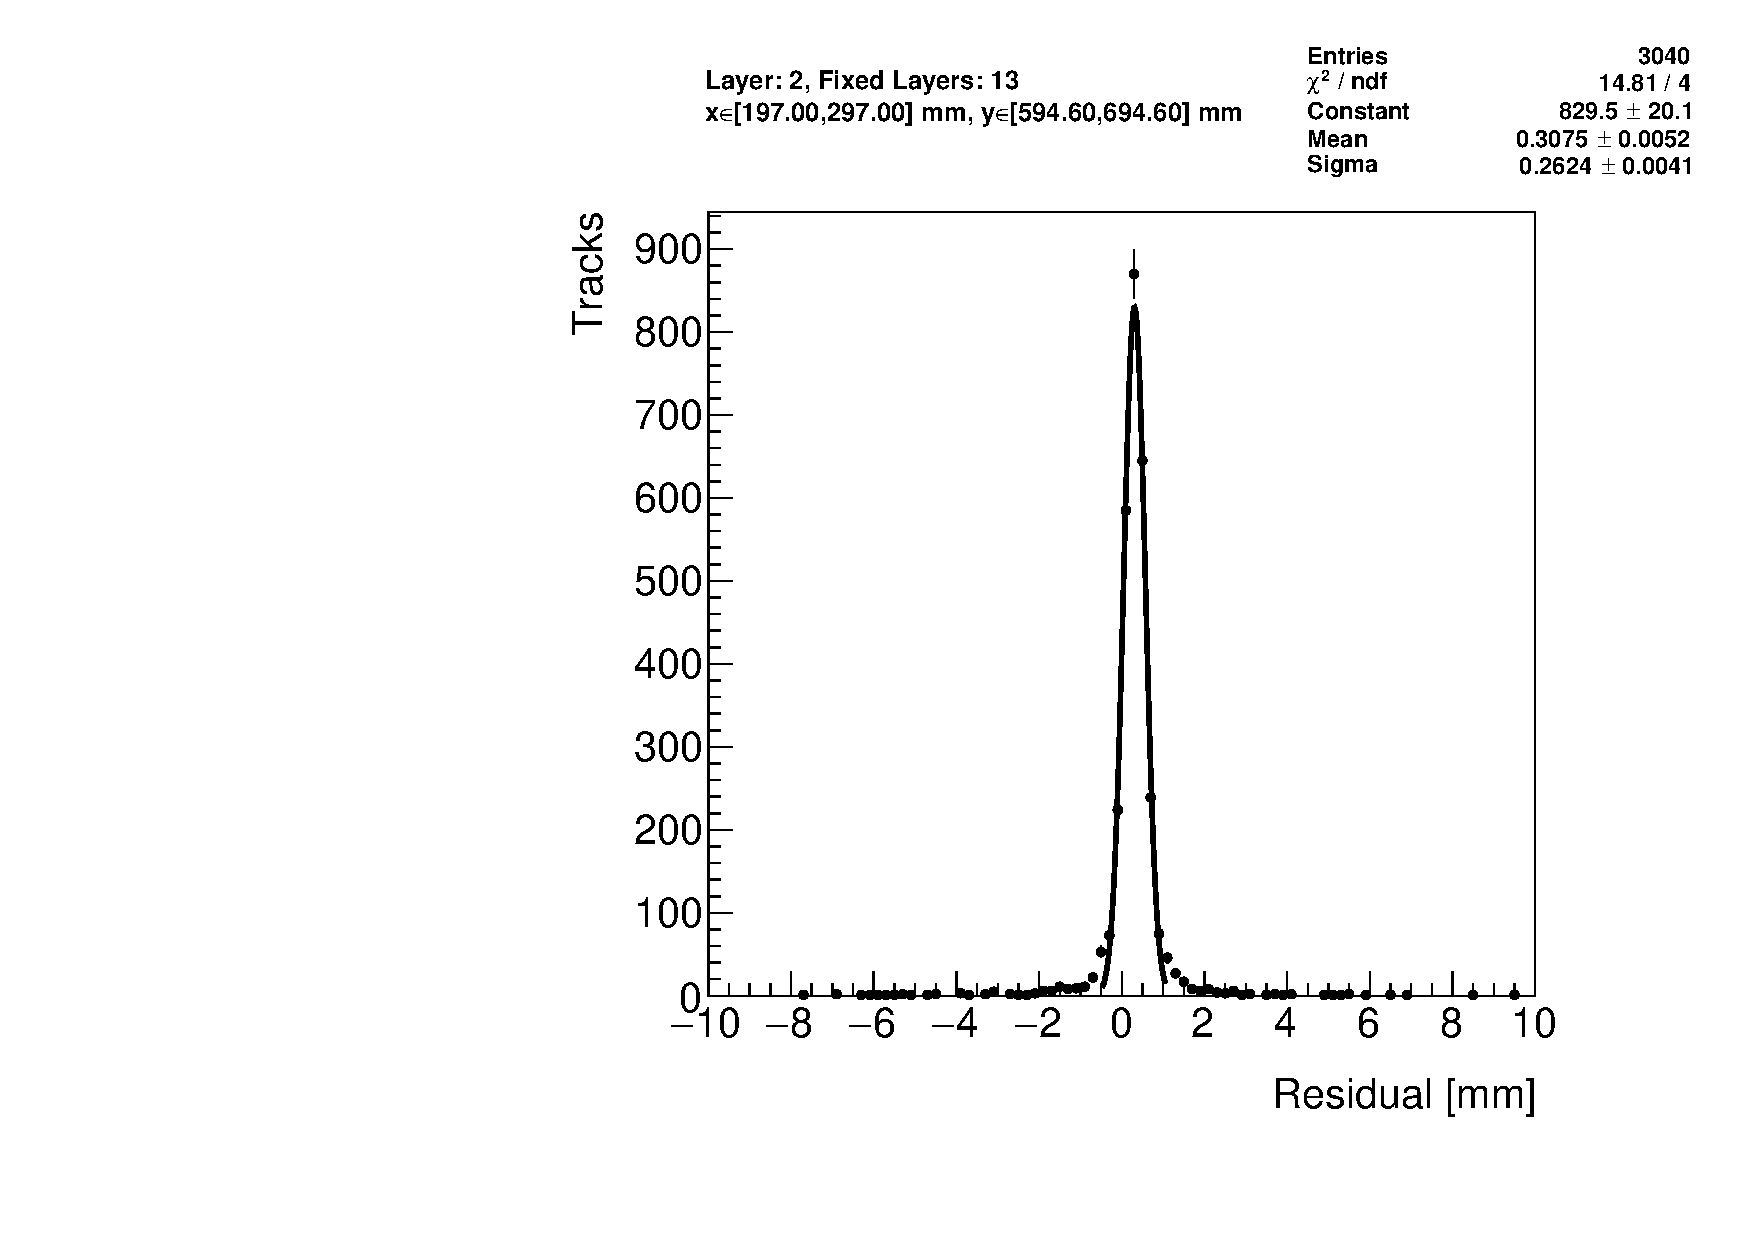
\includegraphics[width=\linewidth]{figures/figure_res_dist_QL2P11_3100V_2021-08-05_xbin_12_ybin_7_layer2_fixedlayers13.pdf}
  \caption{Tracks on layer 2, reference layers 1 and 3.}
  \label{fig:res_dist_L2_F13}
\end{subfigure}%
\begin{subfigure}{.5\textwidth}
  \centering
  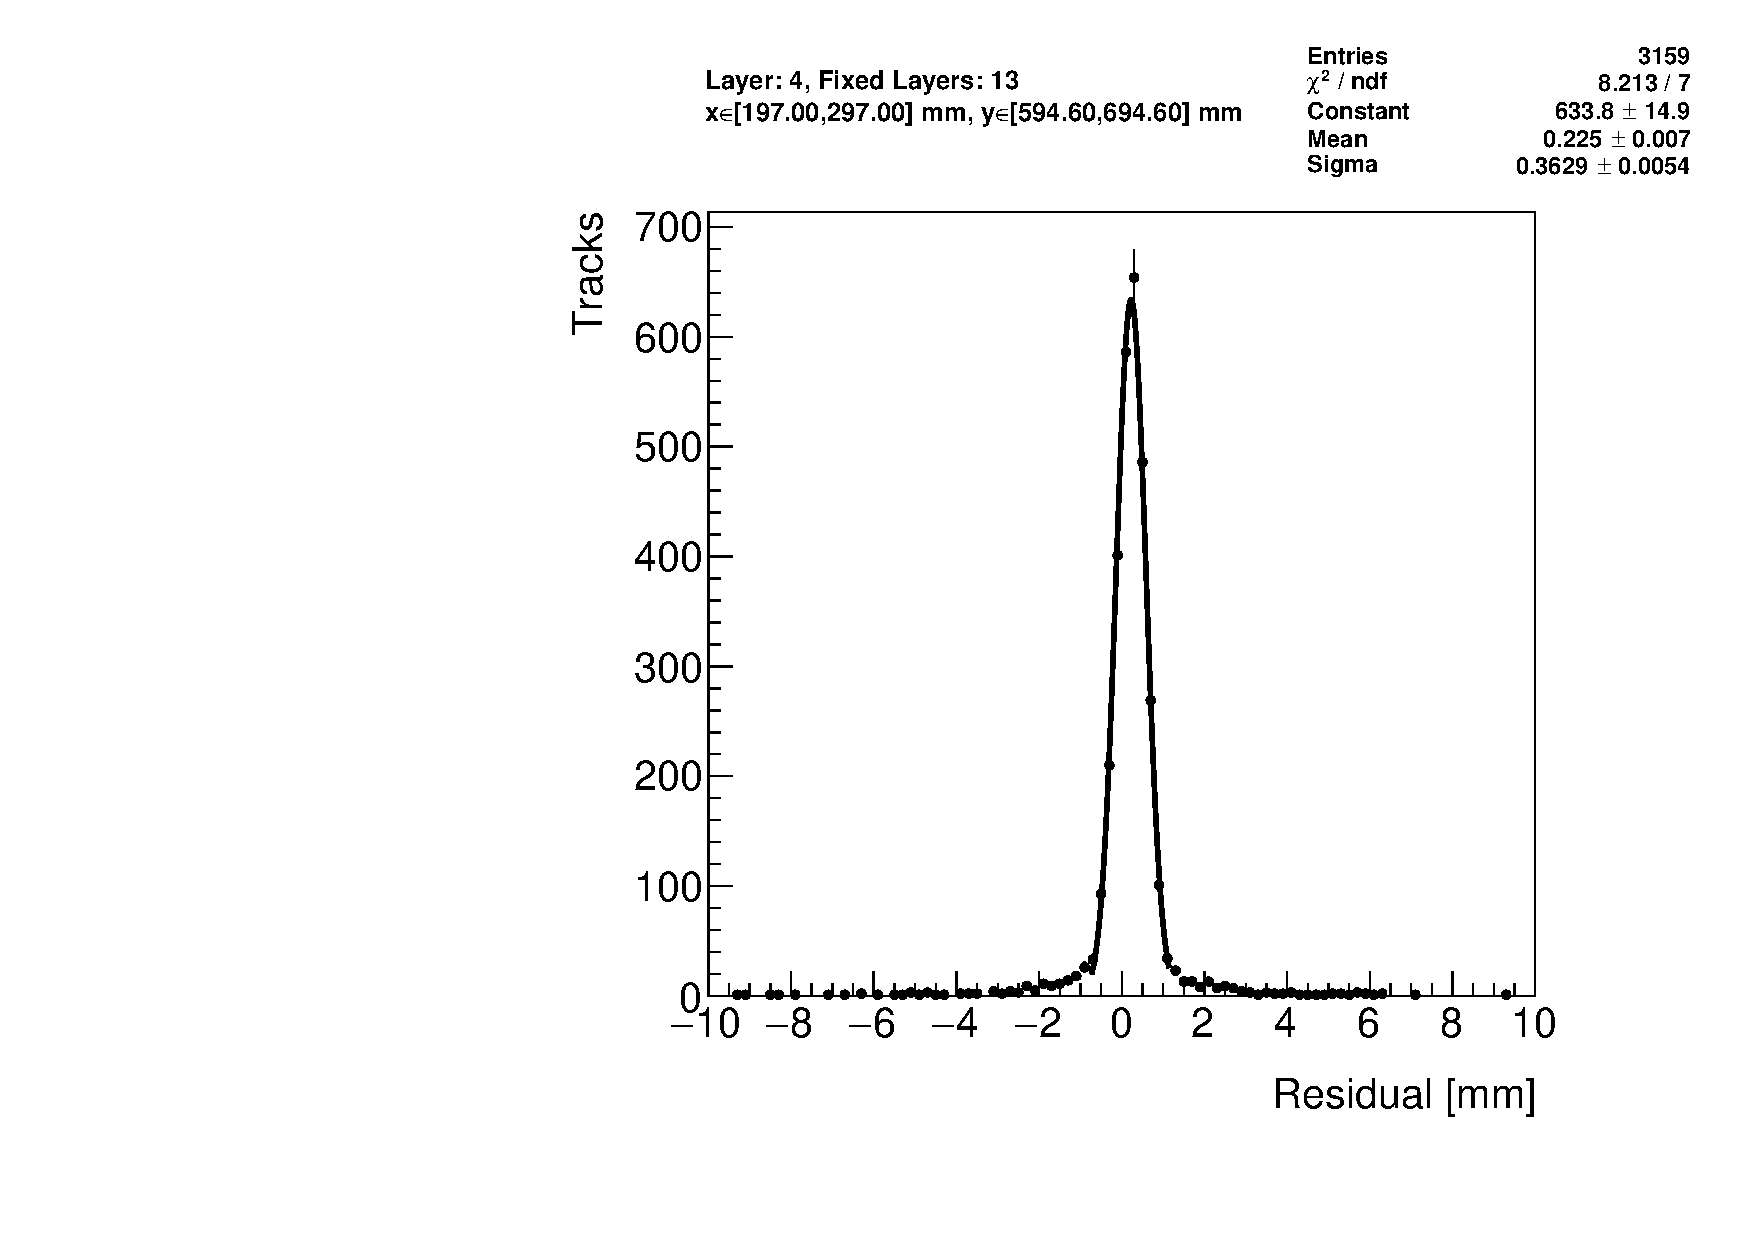
\includegraphics[width=\linewidth]{figures/figure_res_dist_QL2P11_3100V_2021-08-05_xbin_12_ybin_7_layer4_fixedlayers13.pdf}
  \caption{Tracks on layer 4, reference layers 1 and 2.}
  \label{fig:res_dist_L4_F12}
\end{subfigure}
\caption{Residual distribution in the region $x\in\left[197, 297\right],  y\in\left[594.6, 694.6\right] mm$ (100 mm by 100 mm area) for two different tracking combinations. }
\label{fig:res_dist}
\end{figure}

The residual distributions were wider for tracking combinations where the extrapolation lever arm was largest. In general, residual means calculated with geometrically less favourable tracking combinations have larger statistical and systematic uncertainties. The bin size of \SI{200}{\micro\meter} for the distributions shown in figure~\ref{fig:res_dist} was chosen based on the uncertainty on residuals calculated from tracks on layer 4 (1) built from hits on layers 1 and 2 (3 and 4) given a cluster y-position uncertainty of \SI{60}{\micro\meter} (appendix~\ref{sec:appendix_clustering_track_residuals}), since these tracks yield residuals with the largest uncertainties.

A gaussian fit was used to extract the mean of the residual distributions. Theoretically, a double gaussian distribution is more apt, but for this analysis the gaussian fit was sufficient, as discussed in appendix~\ref{appendix:systematics_res_fit_fcn}.

The area of the region of interest was \SI{100}{\milli\meter} by \SI{100}{\milli\meter}. The size balanced the amount of tracks falling in the region of interest to give sufficient statistics to the local residual distributions, while being smaller than the order on which misalignments were expected to effect the local offsets significantly. "Significantly" in this context was defined based on the distance in $x$ that a large but possible rotation of \SI{1000}{\micro\radian} would change the local offset by more than \SI{50}{\micro\meter}, which is half the required position resolution of the sTGCs~\cite{nsw_tdr}.

It is only possible to calculate relative local offsets with cosmics data because there was no external reference to measure positions on all layers with respect to. As an example, assuming that the residual on layer 2 in figure~\ref{fig:fake_event_display} is representative of the relative local offset, the residual on layer 2 could be caused by layer 2 being misaligned from nominal, but it could also be caused by layers 1 and 4 being misaligned from nominal while layer 2 is in its expected position! Any number of combinations of local offsets on layers 1, 2 and 4 could produce the residual on layer 2. The value of relative local offset measurements will be shown and discussed throughout this work.

% --------------------------------------------------
\section{Visualizing relative misalignments between layers}
% --------------------------------------------------

The mean of residuals was extracted for regions across entire quadruplet layers for every tracking combination to get a picture of the relative misalignments between layers. 

\begin{figure}
\centering
\begin{subfigure}{0.85\textwidth}
  \centering
  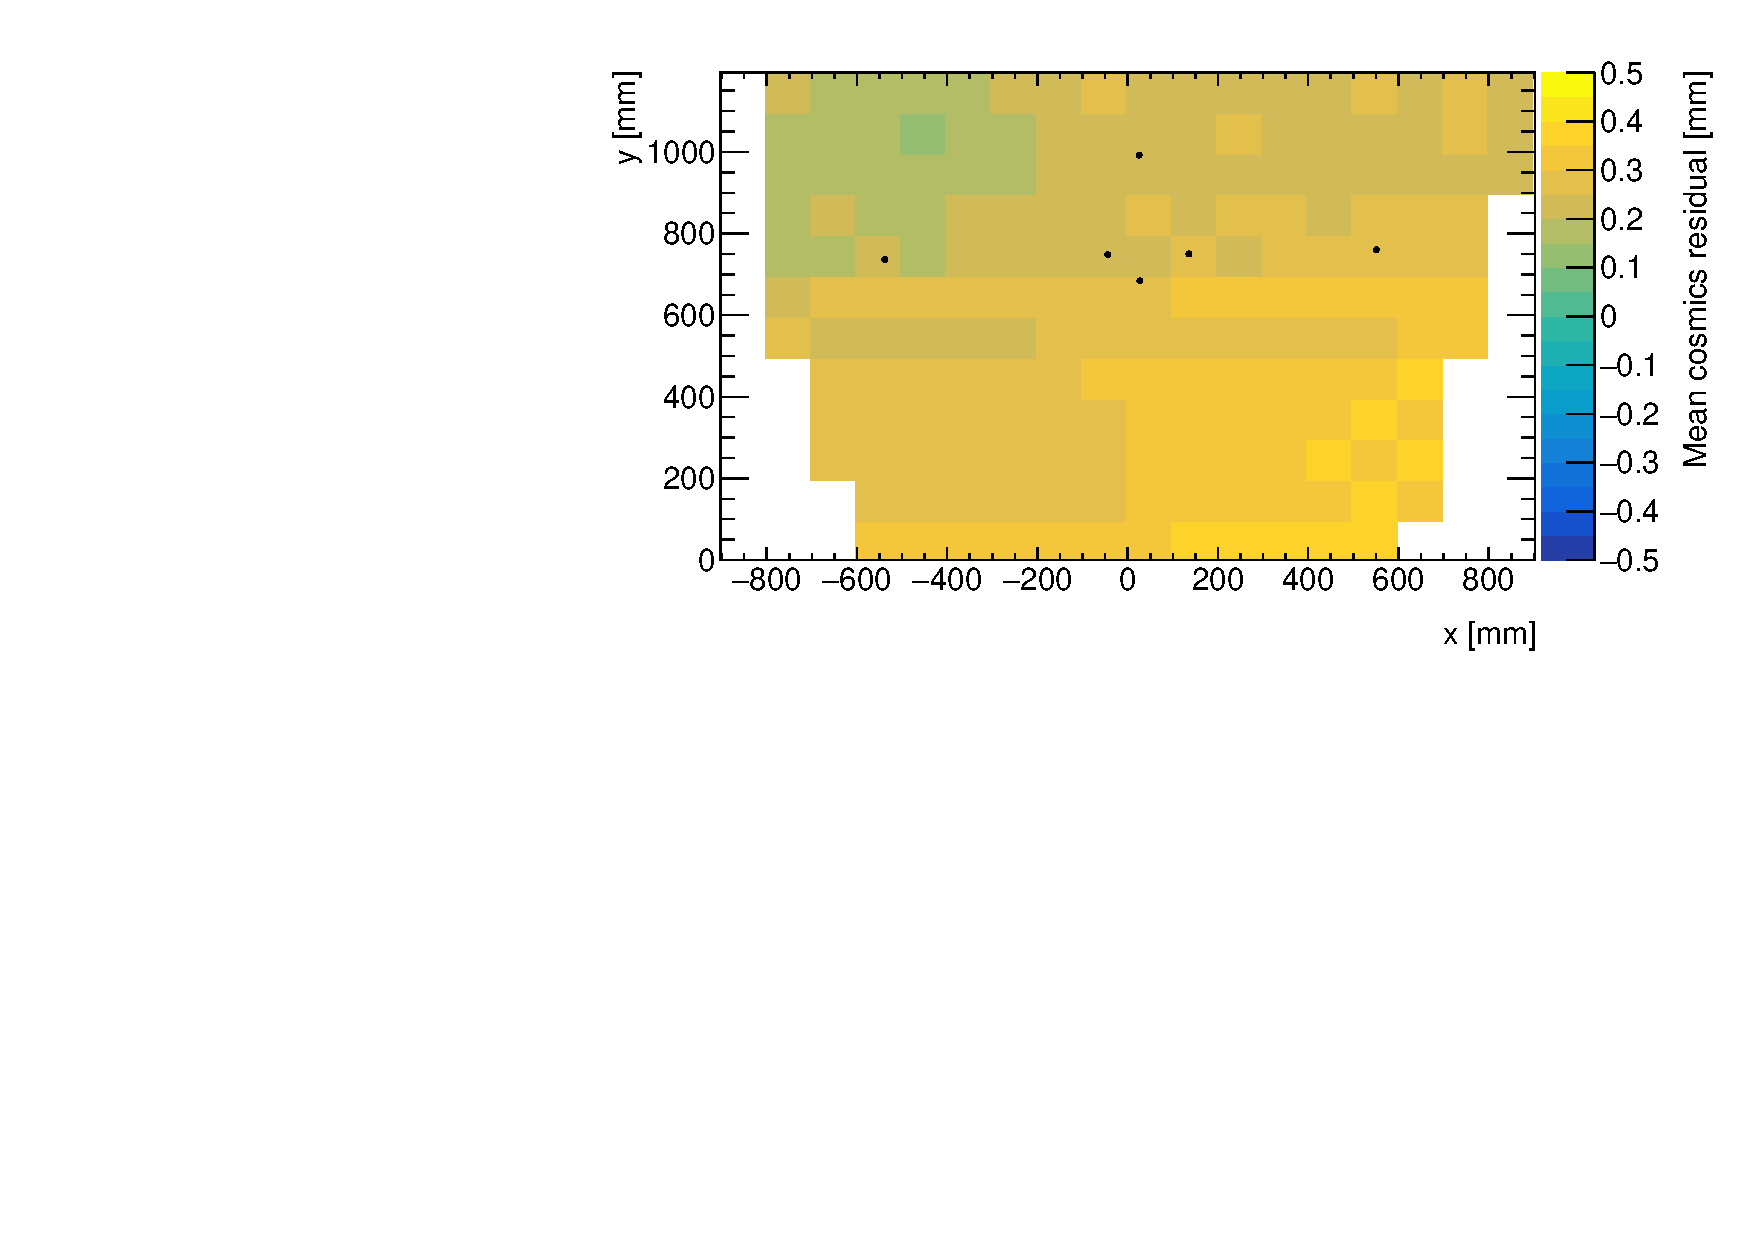
\includegraphics[width=\linewidth]{figures/figure_QL2P11_3100V_2021-08-05_fit_means_xray_overlay_layer2_fixedlayers13.pdf}
  \caption{Mean of residuals for tracks on layer 2, reference layers 1 and 3.}
  \label{fig:res_mean_th2_L2_F13}
\end{subfigure}%
\vspace*{\floatsep}
\begin{subfigure}{0.85\textwidth}
  \centering
  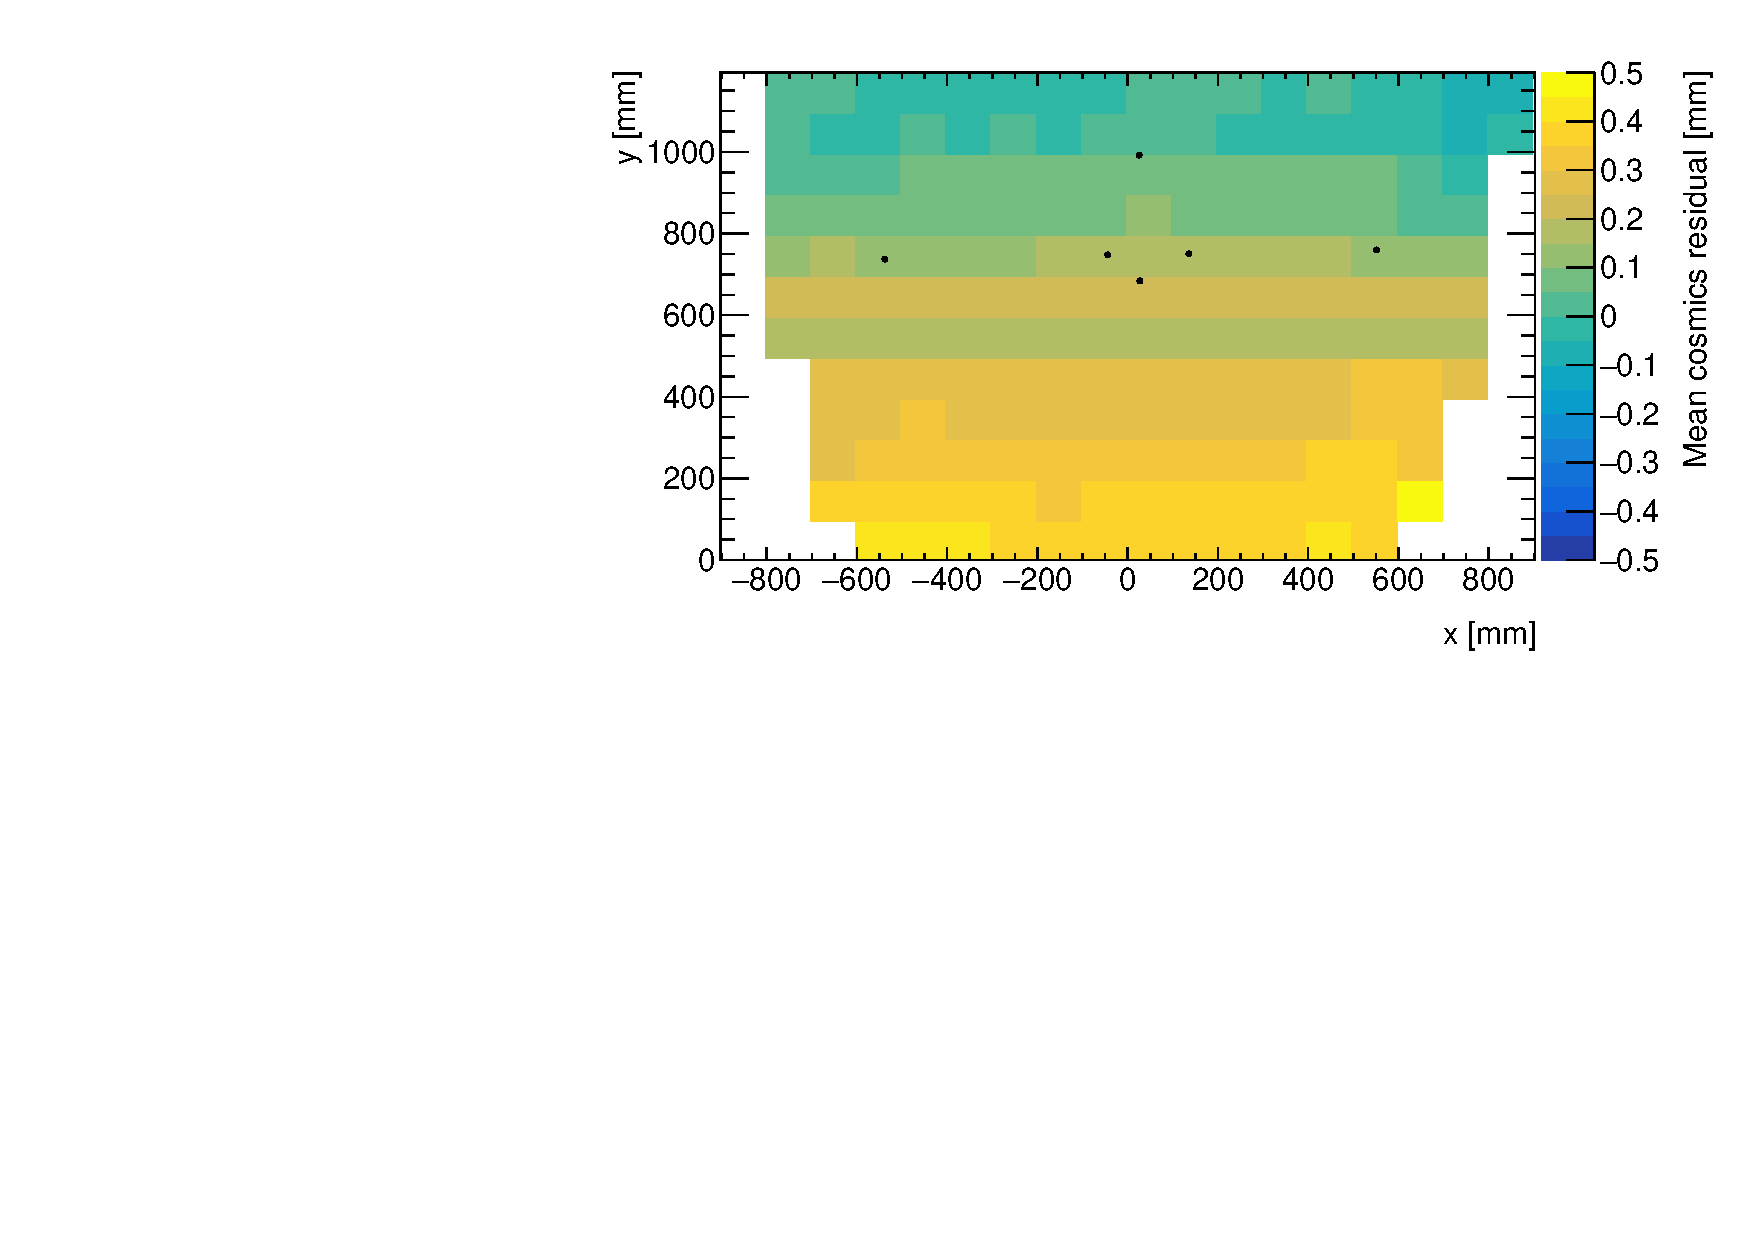
\includegraphics[width=\linewidth]{figures/figure_QL2P11_3100V_2021-08-05_fit_means_xray_overlay_layer4_fixedlayers13.pdf}
  \caption{Mean of residuals for tracks on layer 4, reference layers 1 and 3.}
  \label{fig:res_mean_th2_L4_F13}
\end{subfigure}
\caption{Mean of residuals in each \SI{100}{\milli\meter} by \SI{100}{\milli\meter} bin over the area of the quad layer for QL2.P.11. The black points represent x-ray survey positions, discussed in chapter~\ref{chap:comparison}.}
\label{fig:res_mean_th2}
\end{figure}

Figure~\ref{fig:res_mean_th2} contains the mean of residuals on layers 2 and 4 with tracking reference layers 1 and 3. Many of the residual means are non-zero, and change smoothly over the layer, indicating that there are relative misalignments. Given that the residual mean changes with $x$ in figure~\ref{fig:res_mean_th2_L2_F13}, there is likely a rotation of layer 2 with respect to layers 1 and 3, combined with an offset of the entire layer. For layer 4 in figure~\ref{fig:res_mean_th2_L4_F13}, perhaps there is a scaling~\cite{carlson_results_2019} of the strip pattern with respect to layers 1 and 3. The interpretation of the patterns in the residual means depends on the choice of misalignment model.

% --------------------------------------------------
\section{Systematic uncertainty in cosmic residual means}
% --------------------------------------------------

The statistical uncertainty on the local residual means was typically around \SI{10}{} - \SI{20}{\micro\meter}, and appendix~\ref{appendix:statistics} shows that the analysis was not statistically limited by the number of triggers collected for each quadruplet. The systematic uncertainties were more significant. 

Systematic uncertainties were assigned per tracking combination as the RMS of the distribution of the difference in local residual means each calculated with a different analysis choice. For example, the RMS associated with fitting the local residual distributions with a Gaussian or double Gaussian is \SI{25}{\micro\meter} for the geometrically least favourable tracking combinations and the distribution is shown in appendix~\ref{appendix:systematics_res_fit_fcn}. For geometrically similar tracking combinations (like: tracks on layer 1 built from hits on layers 3 and 4, and tracks on layer 4 built from hits on layers 1 and 2), the systematic uncertainty was assigned as the average RMS for both.

Other choices were whether to use data collected at 2.9~kV or 3.1~kV; what cluster fitting algorithm to use; and whether or not to apply a differential non-linearity (DNL) correction to the cluster y-positions. A systematic uncertainty was assigned using the method above to account for the effect of each choice. The reasons for each choice are listed below.

Data taken at 3.1~kV was used over 2.9~kV because the strip and wire tracking efficiency increases with higher voltage~\cite{lefebvre_thesis} (appendix~\ref{appendix:systematics_2900V_vs_3100V}).

The \package{Minuit2} package~\cite{hatlo_developments_2005} was used to fit clusters over Guo's method~\cite{guo_simple_2011} because it provided automatic statistical uncertainty estimates and is the standard choice (appendix~\ref{appendix:systematics_cluster_fit_fcn}).

The DNL correction was not applied because its effect on the residual means was negligible (appendix~\ref{appendix:systematics_dnl}).

A summary of the systematic uncertainties assigned for each tracking combination is given in table~\ref{tab:sys_uncerts}.

\begin{table}

\begin{tabularx}{\textwidth} {
 | >{\raggedright\arraybackslash}X
 | >{\raggedright\arraybackslash}X 
 | >{\raggedright\arraybackslash}X 
 | >{\raggedright\arraybackslash}X 
 | >{\raggedright\arraybackslash}X 
 | >{\raggedright\arraybackslash}X 
 | >{\raggedright\arraybackslash}X | }
 
 \hline
 \textbf{Tracking geometry} & \textbf{Residual distribution fit function (\ref{appendix:systematics_res_fit_fcn})} & \textbf{Cosmics data collection voltage (\ref{appendix:systematics_2900V_vs_3100V})} & \textbf{Cluster fit algorithm (\ref{appendix:systematics_cluster_fit_fcn})} & \textbf{Apply DNL correction or not (\ref{appendix:systematics_dnl})} & \textbf{Total} \\ 
 \hline
 \hline 
   Layer 3, fixed layers 1, 2 - like & 0.01 & 0.04 & 0.02 & 0.01 & \textbf{0.05} \\
 \hline
   Layer 4, fixed layers 1, 2 - like & 0.03 & 0.01 & 0.03 & 0.01 & \textbf{0.10} \\
 \hline
    Layer 2, fixed layers 1, 3 - like & 0.01 & 0.02 & 0.01 & 0.000 & \textbf{0.03} \\
 \hline
    Layer 4, fixed layers 1, 3 - like & 0.01 & 0.04 & 0.01 & 0.01 & \textbf{0.04} \\
 \hline
    Layer 2, fixed layers 1, 4 - like & 0.01 & 0.04 & 0.01 & 0.01 & \textbf{0.04} \\
 \hline
 
\end{tabularx}
\caption{Systematic uncertainty assigned for each analysis option, detailed in appendix~\ref{appendix:systematics}.}
\label{tab:sys_uncerts}
\end{table}

The uncertainty in each mean cosmics residual was assigned as the sum in quadrature of the statistical uncertainty in the mean and the appropriate systematic uncertainty for the tracking combination. Given that the uncertainty in the mean cosmics residuals is lesser than or near to the order of the required position resolution of the sTGCs (\SI{100}{\micro\meter}~\cite{nsw_tdr}) the cosmic residual means are relevant input for alignment studies.
% ==================================================
% CHAPTER 5: Using x-rays to measure relative strip position offsets
% ==================================================

\chapter{Using x-rays to measure relative strip position offsets}
\label{chap:xray}

Local offset measurements were done with the x-ray method. The reader is referred to the paper describing the x-ray method~\cite{lefebvre_precision_2020}, although some minor changes have been made to the experimental setup since it was written. The experimental setup described here is current and was used to collect the data presented in this thesis.
% Makesure to put this in the statement of contribution

% NOTE: Wrote this with information available in JINST, or things I know to be updated (eg. brass holder and collimator). I can guess at other things based on the WedgeAlignment-Production code, but don't actually know. Those things are in iffalse statements.
% --------------------------------------------------
\section{Experimental setup}
% --------------------------------------------------

The x-ray tests were performed after the quadruplets arrived at CERN, were assembled into wedges, and alignment platforms installed. Essentially, an x-ray gun was attached to one of the alignment platforms glued to the surface of the wedge and the x-ray beam profile recorded by the strips.

\begin{figure}
    \centering
    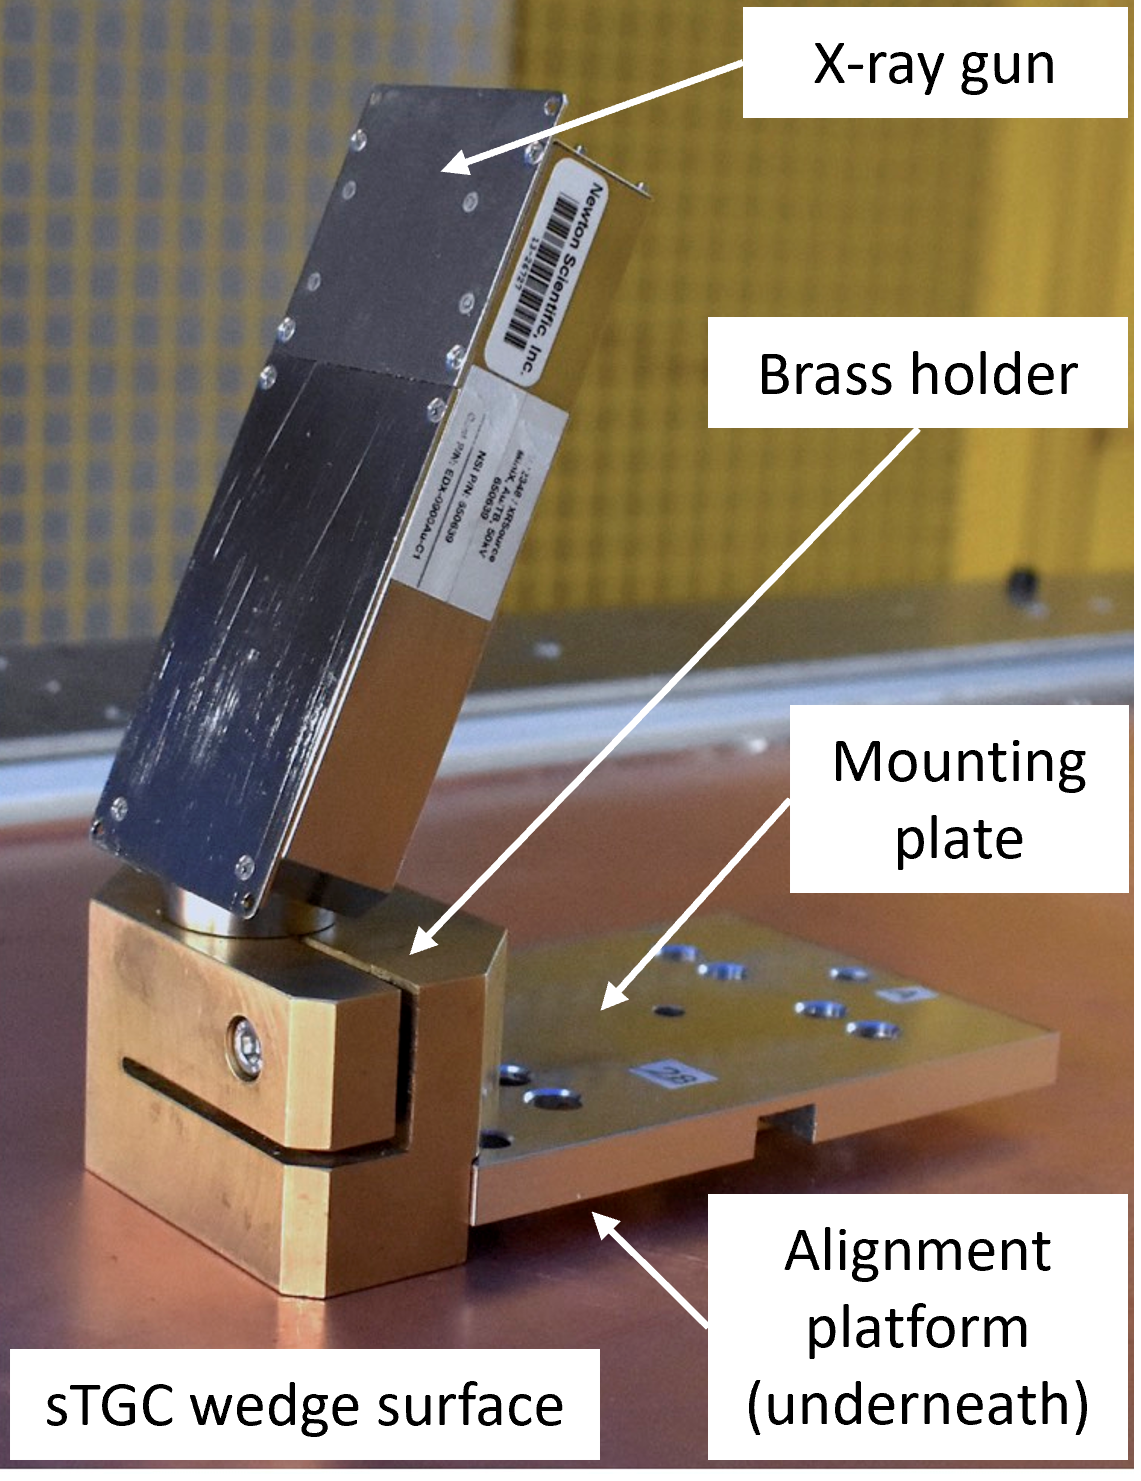
\includegraphics[width = 0.5\textwidth]{figures/xray_setup.png}
    \caption{The x-ray gun mounted to the alignment platform on the surface of the wedge. Adapted from~\cite{lefebvre_precision_2020}.}
    \label{fig:xray_setup}
\end{figure}

The wedges were installed on carts that could rotate their surface to a horizontal position. A mounting platform was installed on top of the alignment platform using a three-ball mount. The x-ray gun used was an \href{https://www.amptek.com/-/media/ametekamptek/documents/resources/specs/mini-x-specifications.pdf?la=en\&revision=512f7eb3-01b3-47fd-864f-5525c850fc6e\&hash=B8B03C0592486E2D91C566C4326F15F5}{Amptek Mini-X tube}. The gun was placed in a brass holder with built-in \SI{2}{mm} collimator and \SI{280}{\micro\meter} copper filter. The holder was mounted on one of five positions on the mounting platform, as shown in figure~\ref{fig:xray_setup}. Gun positions were chosen to avoid wire support structures in the sTGCs that reduce hit efficiency~\cite{lefebvre_thesis} and boundaries between sets of strips read out by two different ASICs that could each have different thresholds. 

As with cosmics data collection, each sTGC also needed gas and high voltage to operate. Each layer was operated at \SI{2.925}{kV} with high voltage from a NIM crate. The chambers were flushed with CO$_2$ before and during data collection.

% The copper filter helped to reduce the effect of attenuation non-uniformities.
The gun produced x-rays with energies under \SI{40}{\kilo\electronvolt} with peaks in the 7-\SI{15}{keV} range. \iffalse Peaks in the 0-\SI{30}{keV} range were filtered out by the copper filter and the copper of the sTGCs. \fi The x-rays mostly interacted with the wedge's copper electrodes and gold-plated tungsten wires via the photo effect. The resulting photoelectrons caused ionization avalanches that were picked up by the strips.
% During ATLAS operation, the position of the source plates will be monitored using the new alignment system~\cite{nsw_tdr}. Therefore, their position will be known in the absolute ATLAS coordinate system. 

% --------------------------------------------------
\section{Data acquisition}
% --------------------------------------------------

A different version of the same front end electronics, but the same ASIC, as used in cosmics testing were used for the x-ray testing to amplify the data and measure the peak signal amplitude. Data was collected for two minutes per gun position with random triggers. A trigger recorded all signals above threshold. \iffalse within \SI{75}{ns} and the signals on neighbouring strips.\fi  Pad and wire data was not recorded.
% Neighbour triggering based on my understanding of the analysis. Does not actually matter for these purposes.

% --------------------------------------------------
\section{Data preparation}
% --------------------------------------------------

Like with cosmics analysis, a default pedestal is subtracted from the signal peak amplitude on each electrode.

Clusters are defined as groups of contiguous strip hits collected within \SI{75}{ns}. The peak signal amplitude of each electrode in a cluster is fit with a Gaussian, and the mean of the Gaussian is taken as the cluster position. Cluster positions are corrected for DNL (see definition in appendix~\ref{appendix:systematics_dnl}). Only clusters composed of hits on 3-5 strips were used in the x-ray analysis. Clusters with signal on more than 5 strips were cut because they were most likely caused by photoelectrons ejected with enough energy to  \iffalse cause more primary ionization and subsequent avalanches ( \fi be $\delta$-rays.
% Note: analysis definitely does the double cluster cut

The x-ray analysis diverges entirely from the cosmics analysis algorithm here because the x-rays do not leave tracks. The signals picked up by the strips are from photoelectrons liberated from the metals of the sTGCs, which only travel through one gas volume and are ejected at all angles. Instead of creating tracks, the cluster position distribution on each layer is used to define the beam profile. A typical beam profile is shown in figure~\ref{fig:xray_beam_profile}.

\begin{figure}
    \centering
    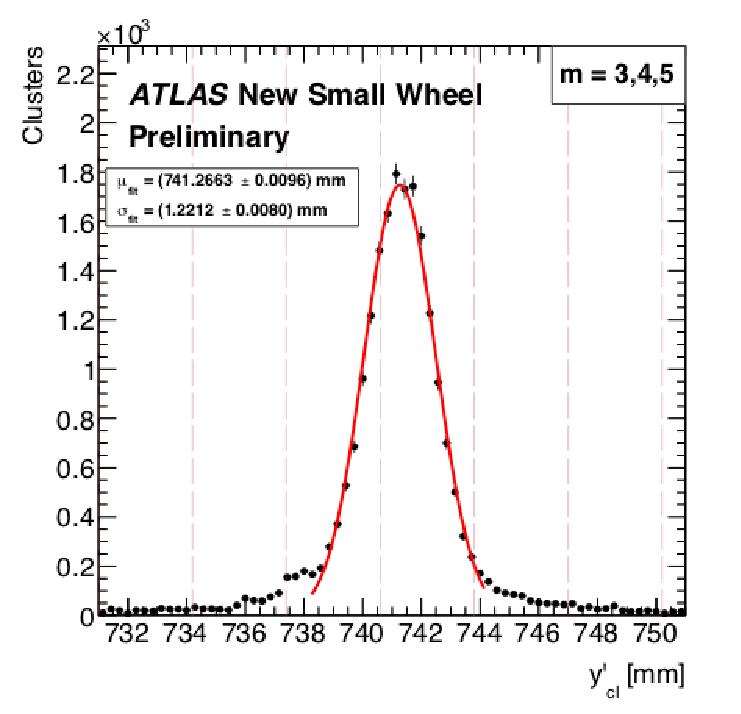
\includegraphics[width = 0.5\textwidth]{figures/figure_xray_beam_profile.pdf}
    \caption{Distribution of x-ray cluster mean positions after the analysis cuts and corrections. The strip cluster multiplicity, $m$, was limited to 3, 4 and 5. The red curve is a Gaussian fit of the distribution and the pink dashed lines denote the edges of the strips~\cite{lefebvre_precision_2020}.}
    \label{fig:xray_beam_profile}
\end{figure}

% --------------------------------------------------
\section{Measuring local offsets}
% --------------------------------------------------
The mean of the cluster position distribution is taken as the x-ray beam profile center. The expected center is calculated assuming a wedge with nominal geometry given the gun position, corrected for: the geometry of the brass holder, the positioning and angle of the alignment platforms and the beam angle. The difference between the expected and reconstructed beam profile center is a measure of the local offset. Applying the logic of equation~\ref{eqn:local_translation} to the beam profile, the Gaussian mean of cluster positions on the given layer acts as the recorded position, $y_i$, the expected center is $y_{nom, i}$ and the local offset is $d_{local, i}$ as before, where $i$ denotes the layer. Since the position of the alignment platforms will be monitored by the alignment system in ATLAS~\cite{nsw_tdr}, the position of the strips that should have been at he gun position are shifted by $d_{local, i}$ and so are known in the ATLAS coordinate system for every position where x-ray data was taken.

The x-ray working group accepted an uncertainty of \SI{120}{\micro\meter} on the beam profile centers. The largest uncertainty comes from the effect of the gun angle, which proved difficult to measure and correct for.

The local offsets are not presented here as the author did not conduct this work. However, the author used the local offsets to calculate relative local offsets.

% --------------------------------------------------
\section{Measuring relative local offsets}
% --------------------------------------------------

The x-ray local offsets were shown to be correlated with the local offsets calculated from the CMM data, but the CMM data does not include the effect of inter-layer misalignments so the degree of correlation measurable was limited. Cosmics data is affected by inter-layer misalignments. Since the local offsets for x-rays and cosmics data are measured in different coordinate systems, they cannot be compared directly. Bringing the cosmics relative local offsets into an absolute coordinate system is impossible; however, the x-ray local offsets can be brought into a relative coordinate system.

The measured x-ray beam profile centers were systematically affected by local offsets in the same way as the mean cosmics residuals, as modeled by equation \ref{eqn:local_translation}. Therefore, if a 2-layer track is built from the beam profile centers on each layer and the residual calculated on a third layer, that residual should match the local mean cosmics residual. The residual is the difference between the beam profile center on the layer of interest and the polated track position from the beam profile centers recorded on the two fixed layers. The beam profile center on the layer of interest acts as $y_{i}$ and the polated track position acts as $y_{track, i}$ in equation~\ref{eqn:residual}.

The built track is not an actual track of the x-ray beam. A beam profile center is actually the Gaussian mean of all selected mean cluster positions recorded during the x-ray data taking period, not a single hit of a track. Building an ``abstract'' track was necessary because the x-rays cause signal in the chamber via the photoeffect so there were not individual ``x-ray tracks'' to record. In fact the x-ray data could be collected separately for each layer. Nonetheless, since the effect of local offsets on the beam profile centers was the same as their effect on the recorded cosmics cluster positions the difference in algorithm between x-ray and cosmics analysis was allowed. 

For each x-ray survey position, the x-ray residual was calculated for all possible tracking combinations (which required an x-ray beam profile on at least three layers). The x-ray residuals on layer 2 calculated from the beam profile centers recorded on layers 1 and 3 are represented as arrows in figure~\ref{fig:xray_res_th2} as arrows for QL2.P.11 and QL2.P.8.  For QL2.P.11, a negative offset at all x-ray survey positions is clear. % Fix this reference to d_local already

\newpage
\thispagestyle{empty}
\newgeometry{top=0.5in,bottom=0.5in}
\begin{figure}
\centering
\begin{subfigure}{\textwidth}
  \centering
  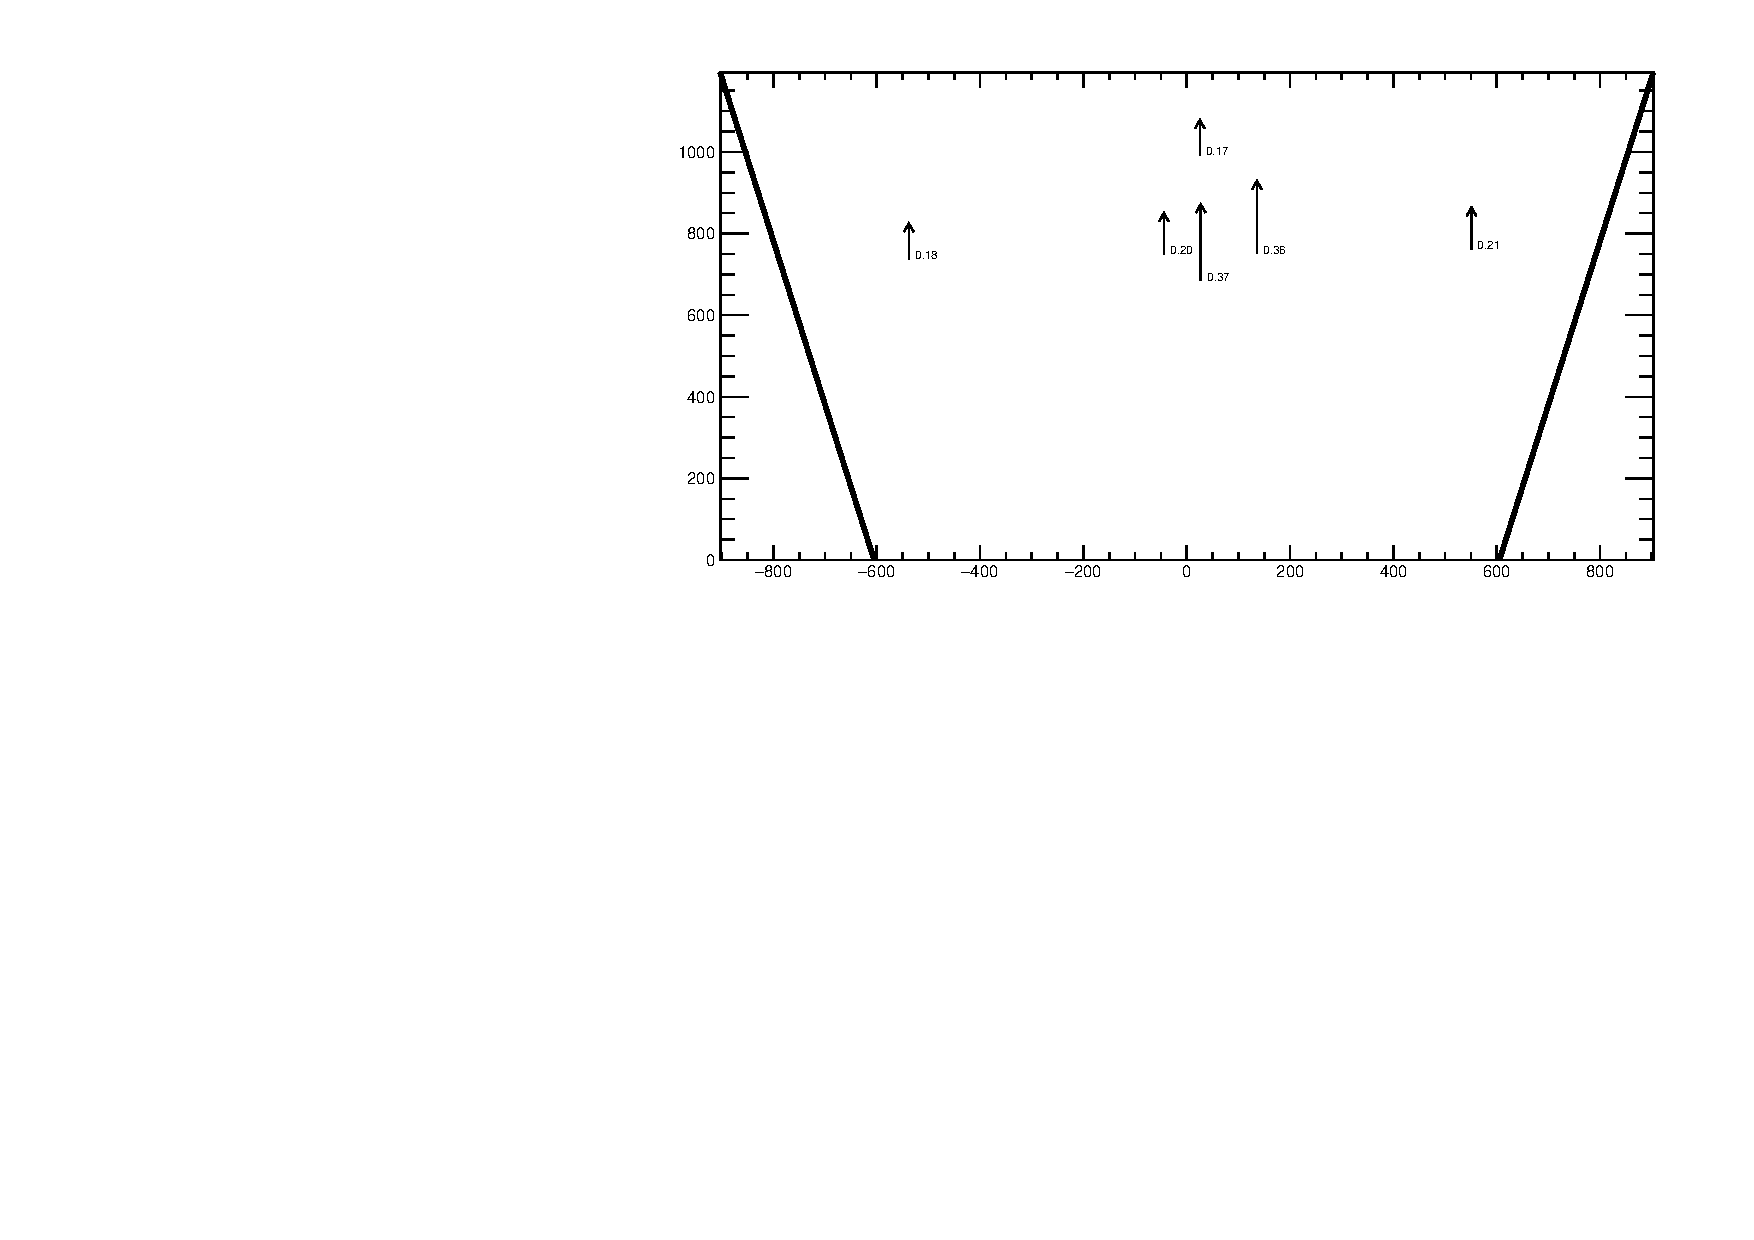
\includegraphics[width=\linewidth]{figures/QL2P11_xray_residuals_layer2_fixedlayers13.pdf}
  \caption{QL2.P.11 x-ray residuals on layer 2, reference layers 1 and 3.}
  \label{fig:xray_res_th2_ql2p11}
\end{subfigure}%
\vspace*{\floatsep}
\begin{subfigure}{\textwidth}
  \centering
  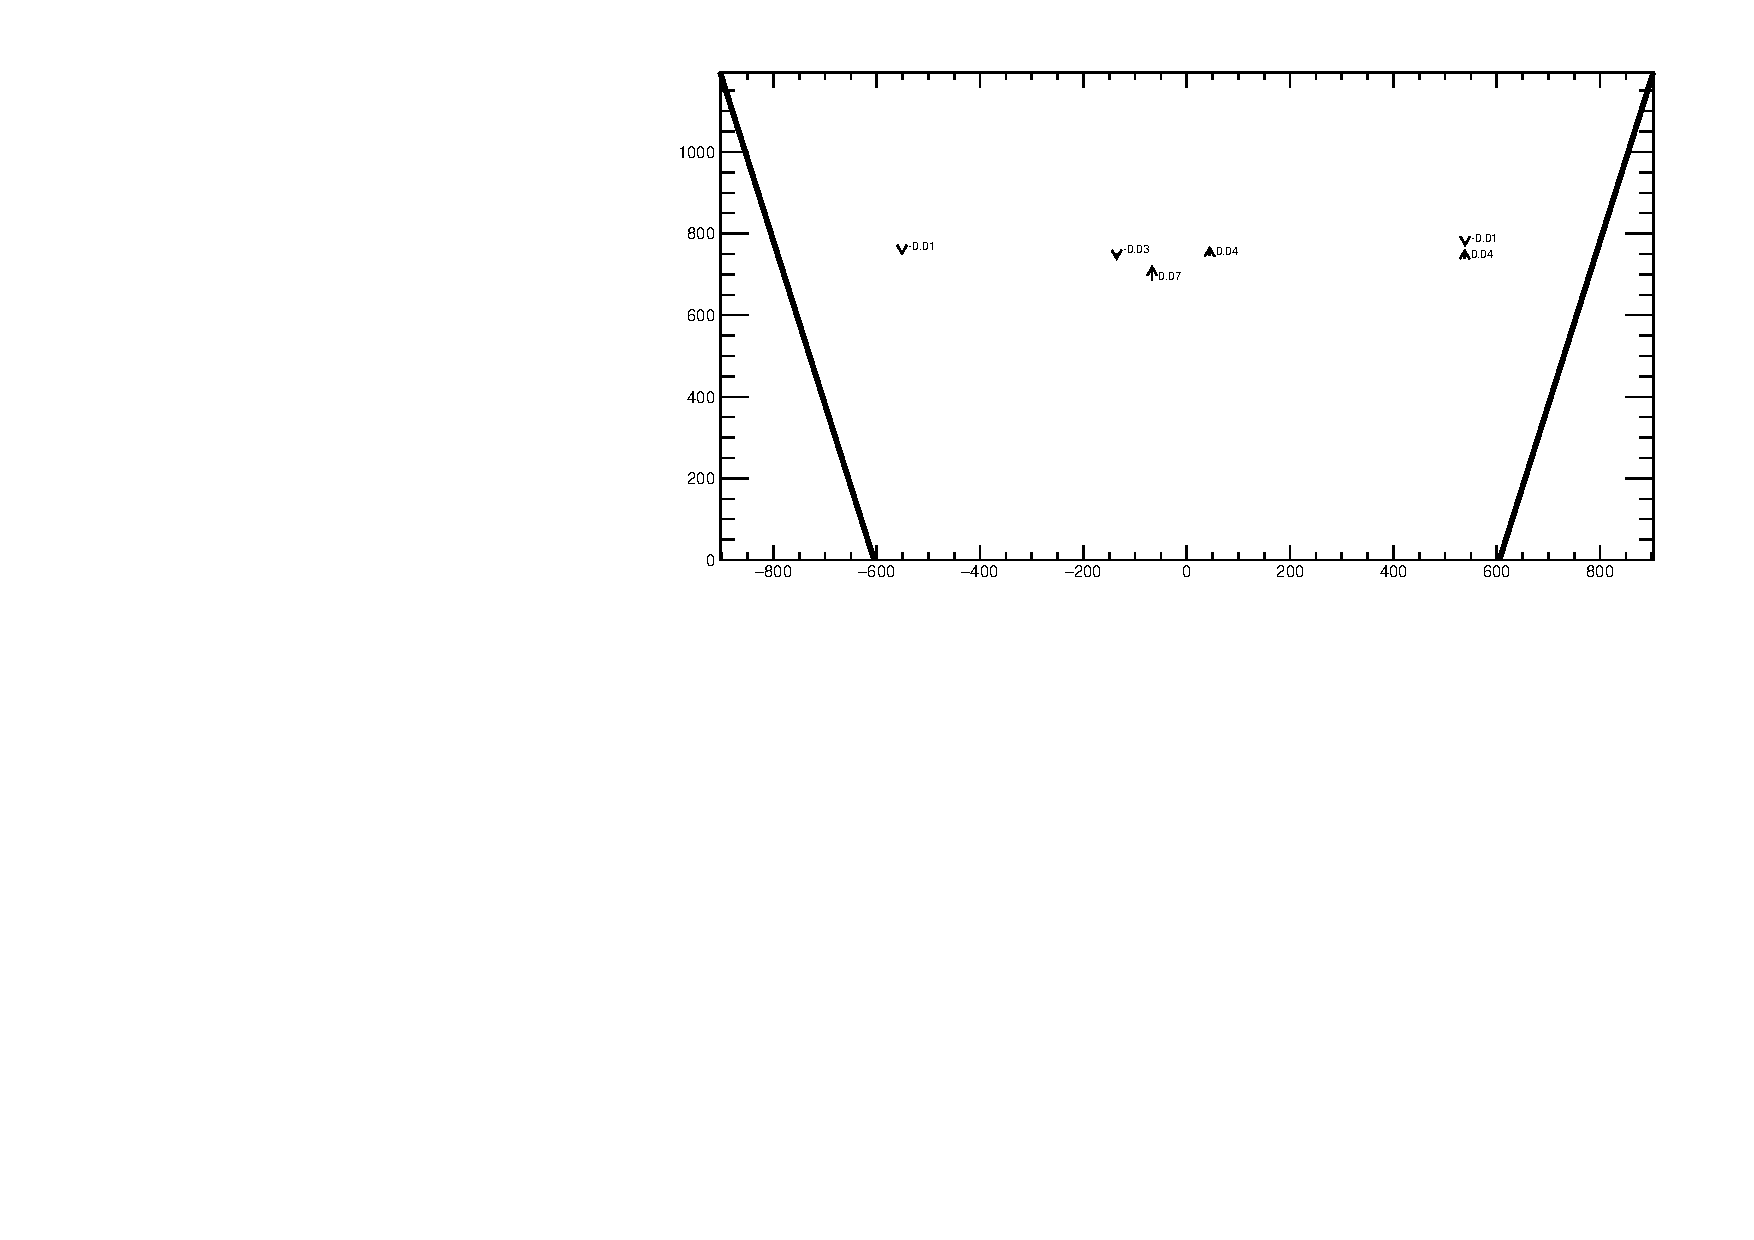
\includegraphics[width=\linewidth]{figures/QL2P08_xray_residuals_layer2_fixedlayers13.pdf}
  \caption{QL2.P.8 x-ray residuals on layer 2, reference layers 1 and 3.}
  \label{fig:xray_res_th2_ql2p8}
\end{subfigure}
\caption{The x-ray residuals on layer 2 calculated from the beam profile centers recorded on layers 1 and 3 for QL2.P.11 and QL2.P.8. The arrows originate from the expected position of the beam profile center assuming a nominal geometry, and the lengths are proportional to the calculated x-ray residuals. The tip of the arrow represents where the recorded hit was with respect to where it should have been recorded nominally. The value of the x-ray residuals are annotated in millimeters and have an uncertainty of $\pm$\SI{0.15}{mm}.}
\label{fig:xray_res_th2}
\end{figure}
\newpage
\restoregeometry

The uncertainty on the x-ray residuals was the error propagated through the tracking, taking an uncertainty of \SI{120}{\micro\meter} on each beam profile center. The uncertainty on the x-ray residuals ranged from \SI{0.15}{mm} to \SI{0.4}{mm} from the most to least geometrically-favourable tracking combination. There is no discernible pattern to the x-ray residuals on QL2.P.8 because they are smaller than the uncertainty. The x-ray residual uncertainties are significantly larger than the uncertainties on the relative local offsets calculated with cosmics data.
% ==================================================
% CHAPTER 6: Comparing cosmic muon and x-ray relative strip position offsets %
% ==================================================

\chapter{Comparing cosmic muon and x-ray relative strip position offsets}
\label{chap:comparison}
% Edit count: Lia - 1, Brigitte - 0

The goal was to validate the local offsets extracted from the x-ray data with cosmics data. The complication was that the x-ray dataset provided absolute local offsets while the cosmics dataset provided relative local offsets, which could not be compared directly. The solution was to analyze the x-ray data in the same relative coordinate system as the cosmics data. The methods and results of the comparison are presented here.

% --------------------------------------------------
\section{Method for comparing x-ray and cosmics data}
% --------------------------------------------------
%TODO : determine if the description of equation 1.1 is suitably general enough to describe the x-ray data

The measured x-ray beam profile centers were systematically affected by local offsets in the same way as the mean cosmics residuals, as modeled by equation \ref{eqn:local_translation}. Therefore, if a 2-layer track is abstracted from the beam profile centers on each layer and the residual calculated on a third layer, that residual should match the local mean cosmics residual. 

The track is "abstracted" because a so-called "beam profile center" is actually the Gaussian mean of all selected mean cluster positions recorded during the x-ray data taking period. Abstracting a track was necessary because the x-rays cause signal in the chamber via the photoeffect so there were not individual "x-ray tracks" to record. In fact the x-ray data was collected separately for each layer. Nonetheless, since the effect of local offsets on the beam profile centers was the same the difference in algorithm between x-ray and cosmics analysis was allowed. 

For each x-ray survey position, the x-ray residual was calculated for all possible tracking combinations (which required an x-ray beam profile on at least three layers). The position of the x-ray residuals are shown as black dots over figure~\ref{fig:res_mean_th2_L2_F13} and \ref{fig:res_mean_th2_L4_F13}. Note that the mean of cosmics residuals around the x-ray points were calculated in bins exactly centered on the nominal x-ray gun position, unlike in figure~\ref{fig:res_mean_th2}.

%---------------------------------------------------
\section{Assessing correlation}
%---------------------------------------------------
\label{sec:assessing_correlation}
Scatter plots of the x-ray and mean cosmics residuals for two sample quadruplets in figures~\ref{fig:correlation} and \ref{fig:no_correlation} reveal the degree of correlation between the datasets.

\begin{figure}
    \centering
    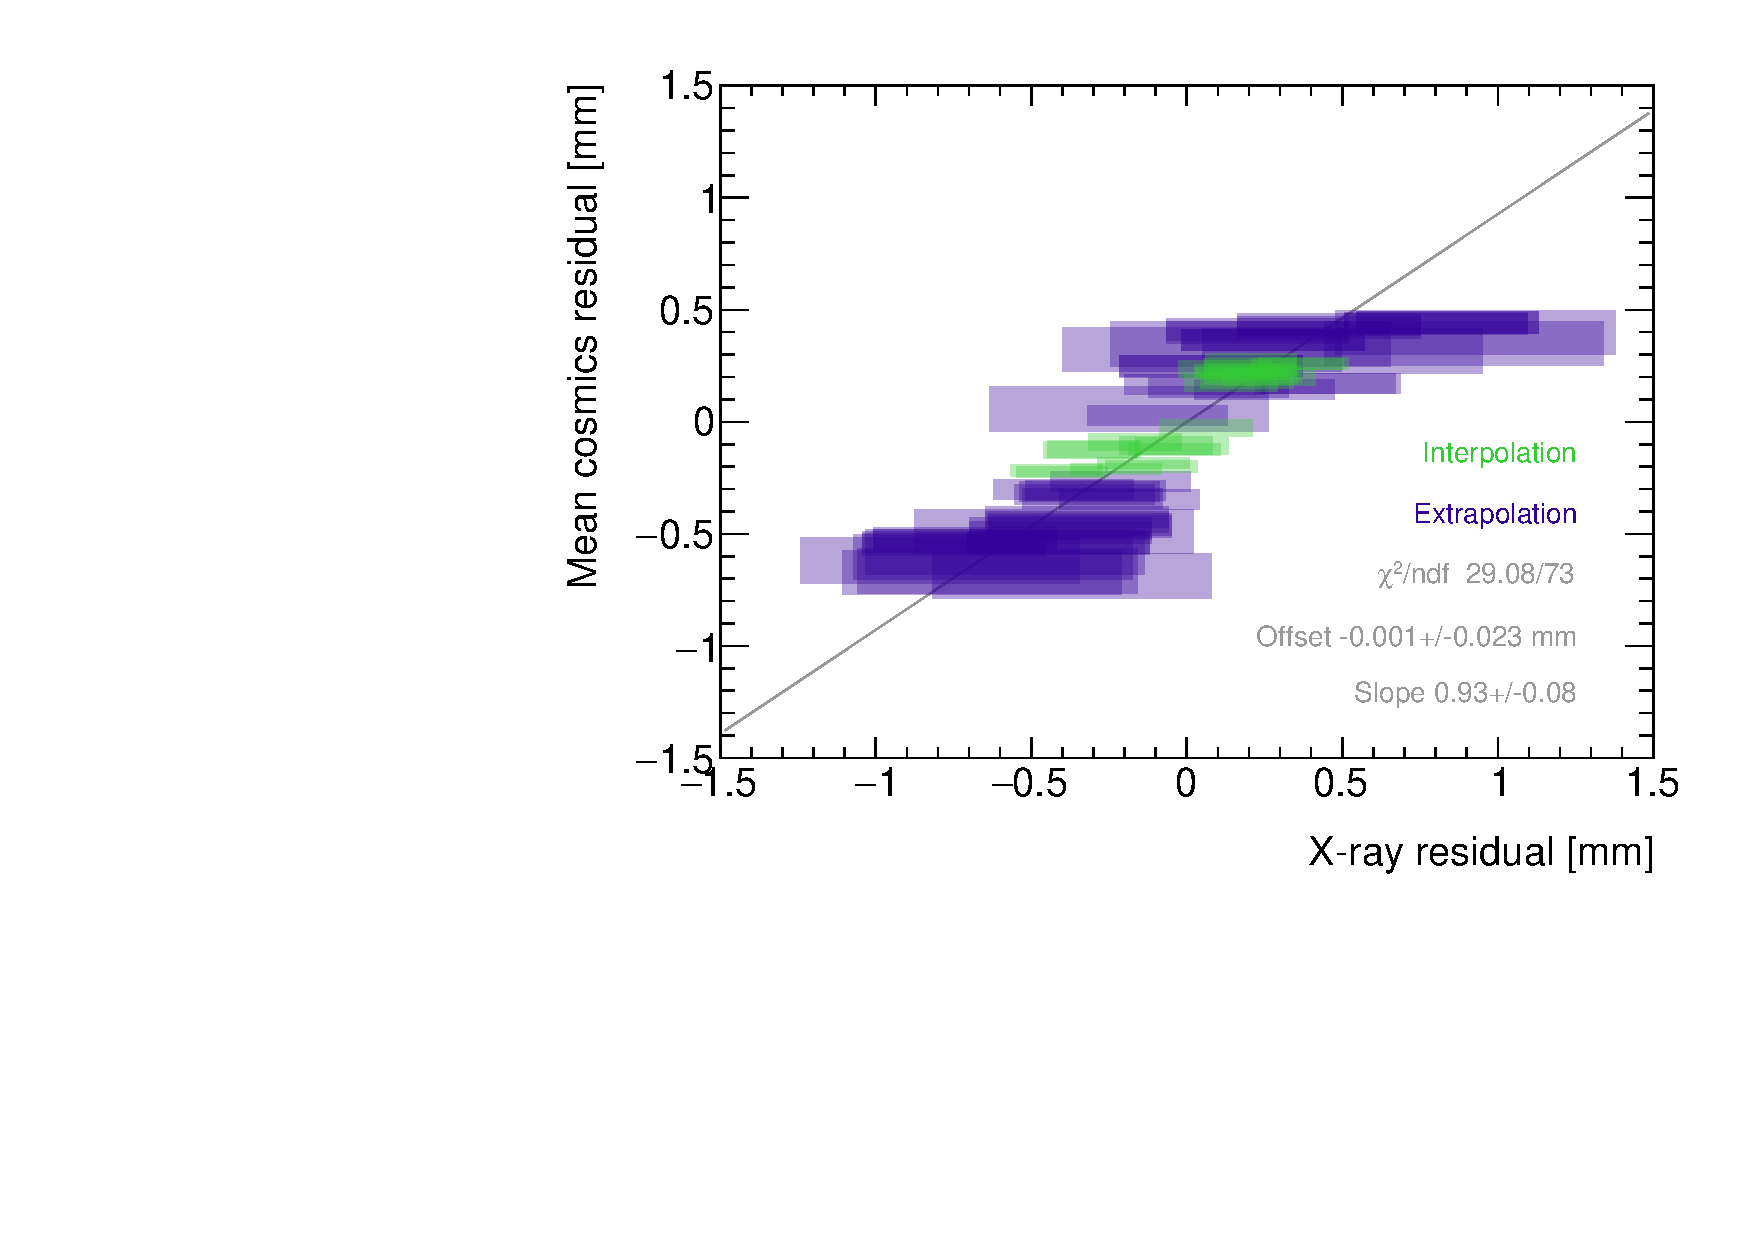
\includegraphics[width = \textwidth]{figures/figure_QL2P11_3100V_2021-08-05_QL2P11_local_cosmic_and_xray_data_correlation_plot.pdf}
    \caption{Correlation plot between x-ray and cosmics residuals for all tracking combinations for QL2.P.11. Each rectangle is centered on an x-ray and mean cosmics residual pair. The width of the rectangles in $x$ and $y$ are the uncertainty in the x-ray and mean cosmics residual respectively. A printer-friendly version of this plot is available in appendix~\ref{appendix:print}.}
    \label{fig:correlation}
\end{figure}

First, the fitted slope and offset in figure~\ref{fig:correlation} show that the two QL2.P.11 datasets are correlated. However, the magnitude of the uncertainties in the x-ray residuals is large (up to half a millimeter) since it comes from propagating the \SI{120}{\micro\meter} uncertainty in the beam profile centers. The large uncertainty set a limit on the sensitivity of the analysis, for if the absolute value of the x-ray residuals of a quadruplet were smaller than the x-ray residual uncertainties, no conclusion about the correlation could be drawn, like for QL2.P.8 (figure~\ref{fig:no_correlation}).

\begin{figure}
    \centering
    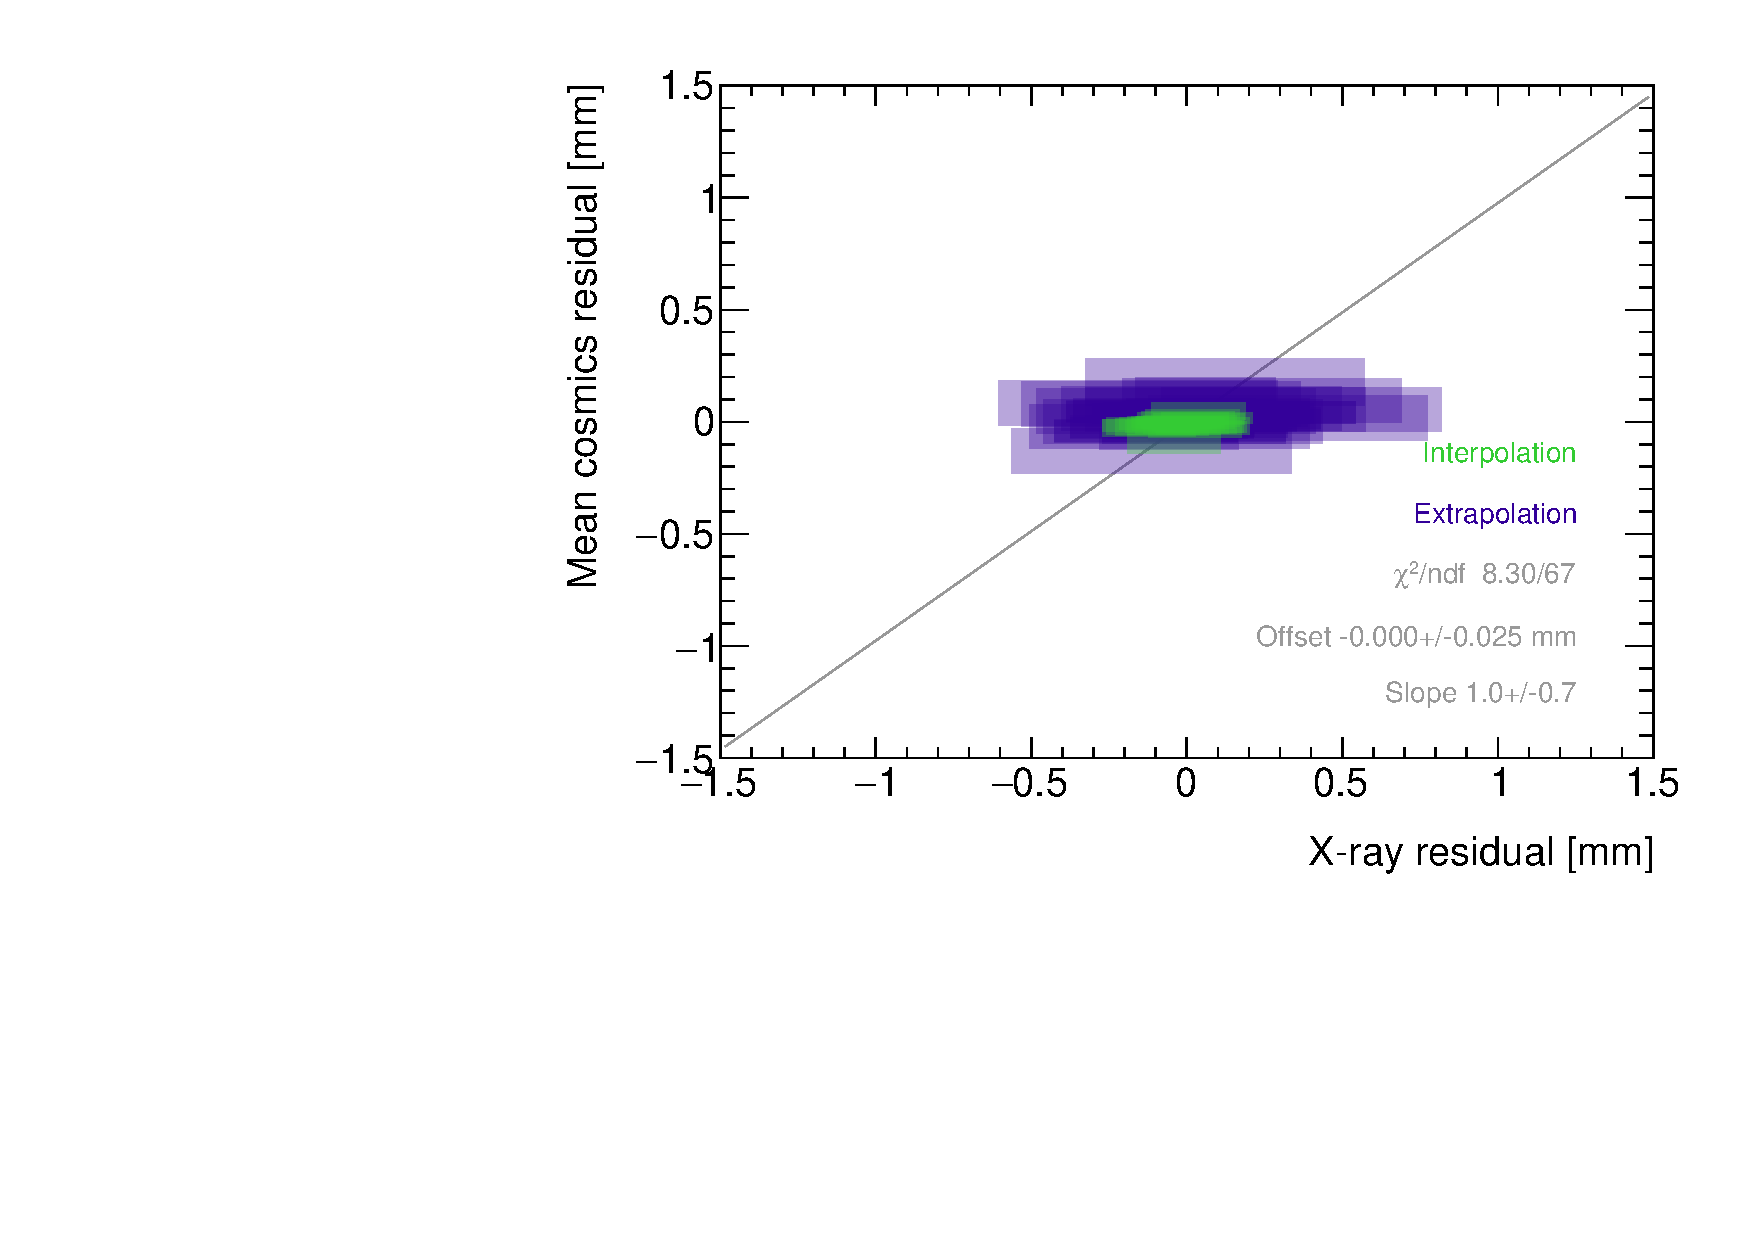
\includegraphics[width = \textwidth]{figures/figure_QL2P08_3100V_2021-08-16_QL2P08_local_cosmic_and_xray_data_correlation_plot.pdf}
    \caption{Correlation plot between x-ray and cosmics residuals for all tracking combinations for QL2.P.8. Each rectangle is centered on an x-ray and mean cosmics residual pair. The width of the rectangles in $x$ and $y$ are the uncertainty in the x-ray and mean cosmics residual respectively. A printer-friendly version of this plot is available in appendix~\ref{appendix:print}.}
    \label{fig:no_correlation}
\end{figure}

Several quadruplets were tested for each quadruplet construction geometry built in Canada: QL2P, QL2C, and QS3P. Each quadruplet fell into one of the two categories: residuals large enough to see a correlation, or residuals too small to see a correlation. Since the x-ray and mean cosmics residuals were measures of the relative local offsets between the layer of a quadruplet and the two reference layers, quadruplets with the most relative misalignment had the largest range of residuals. So, the correlation plots were an easy visual way to identify quadruplets with large relative misalignments.

There are three patterns in the residuals on the scatter plot explained by geometry. First, for both datasets the uncertainty in the extrapolated track residuals were larger than the interpolated track residuals because of the extrapolation lever arm. For the x-ray residuals, the effect of the lever arm on the uncertainty was direct since the residual was calculated from a single abstracted track; for the cosmics residuals it was the widening of the residual distribution on the layer of interest due to the extrapolation lever arm that increased the statistical uncertainty in the fitted mean of residuals. Second, residuals calculated through extrapolation tend to be larger because the extrapolation lever arm can produce more extreme values. Third, the pattern of points in figure~\ref{fig:correlation} is slightly mirrored. This is expected since the residuals calculated for a given set of three layers are geometrically correlated. 

The correlation of the cosmics residuals with the x-ray residuals alone does not validate the method; all the studies in described in appendices~\ref{appendix:statistics} and ~\ref{appendix:systematics} demonstrate its robustness. The analysis could be validated externally by comparing the mean cosmics residuals to the relative misalignment parameters calculated using \package{tgc\_analysis/MatrixMethod}~\cite{lefebvre_tgc_analysis} and JOHN FLORES CHI2 METHOD.

% --------------------------------------------------
\section{Limitations}
% --------------------------------------------------
The most important limit on measuring the degree of correlation between the x-ray and cosmics residuals was the uncertainty on the x-ray residuals, which stemmed from the systematic uncertainty in the x-ray beam profile centers~\cite{lefebvre_precision_2020}. The method was limited primarily by the sTGCs' poor x-ray position resolution, since x-rays do not create real tracks anyways. 

The analysis of certain quadruplets was also limited by the availability of data. Sometimes, less than three layers were surveyed for a given x-ray gun position so no residuals could be calculated. Too few x-ray residuals prevented the analysis from detecting a significant correlation. Often, the analysis of smaller quadruplets suffered as a result because they had fewer alignment platforms, and hence gun positions, on their surfaces. In addition, the analysis was limited to certain quadruplets. The wedges constructed the earliest (typically small wedges) were surveyed when the method was still being designed and so have limited x-ray residuals calculated from beam profiles of lower quality. Also, not all cosmic muon test sites had enough front end electronics to collect data on three layers simultaneously, which is the minimum required to be able to calculate residuals.

Nonetheless, the comparison of x-ray and cosmics residuals was really to confirm the x-ray method's ability to measure local offsets with an independent dataset; the analysis of quadruplets with relative misalignments large enough to detect a correlation achieved this goal.

% ==================================================
% CHAPTER 7: Summary and Outlook %
% ==================================================

\chapter{Outlook and summary}
\label{chap:outlook_and_summary}
% Edit count: Lia - 1, Brigitte - 0

The cosmic muon dataset was used to independently confirm the absolute local offsets measured by the x-ray method. The x-ray offsets are being used to complete the sTGC alignment scheme of the NSWs: the NSW alignment system monitors the position of alignment platforms on the surface of sTGC wedges, and the x-ray measurements provide the offsets of the strip pattern with respect to each alignment platform. The continuation of this analysis is detailed next (section~\ref{sec:outlook}) before considering the larger context (section~\ref{sec:summary}). 

% --------------------------------------------------
\section{Outlook}
% --------------------------------------------------
\label{sec:outlook}

Next all quadruplets with suitable cosmics and x-ray data should be surveyed to flag anomalous quadruplets (as a first step). If a quadruplet's correlation plot like figure~\ref{fig:correlation} or \ref{fig:no_correlation} reveals an unexpected correlation or has a large scatter, it would indicate an issue with either the cosmics or x-ray data collection to be investigated further. The uncertainty in each set of tracking points would inform the interpretation of the anomaly. Then, the quality of the correlation should be evaluated over all quadruplets instead of individually. 
 
For now, the correlation for the individual quadruplets tested support the use of the x-ray data to build a global alignment model~\cite{lefebvre_precision_2020}. Work on creating an alignment model is ongoing with the development of \package{stgc\_as\_built\_fit}~\cite{lefebvre_stgc_as_built_fit}. Currently, the algorithm compares the y-position of a local group of strips at each x-ray gun position as measured by the x-ray and CMM methods in a fit to extract a global slope ($m$) and offset ($b$) per layer, $l$, where the $\chi^2$ is given by equation~\ref{eqn:chi2}.

\begin{equation}
    dy_{cmm, corr} = y_{cmm} + b_l + m_{l}x - y_{nom}
    \label{eqn:dy_cmm_corr}
\end{equation}
\begin{equation}
    \chi^2 = \frac{\left[dy_{cmm, corr} - dy_{xray}\right]^2}{\delta dy_{xray}^2 + \delta dy_{cmm, corr}^2}
    \label{eqn:chi2}  
\end{equation}

Here, $dy$ refers to the corrected CMM and x-ray local offsets, and $\delta dy$ refers to their respective uncertainties. The CMM measurements were taken before the cathode boards were assembled into quadruplets, so alignment parameters for the given layer were extracted from the $\chi^2$ fit by stepping the corrected CMM y-position towards the x-ray y-position by adjusting the alignment parameters. The plan is that the alignment parameters will be provided to \package{Athena}~\cite{the_atlas_collaboration_athena} to precisely reconstruct muon tracks from the NSWs' sTGCs. The large uncertainty on the x-ray local offsets (\SI{120}{\micro\meter}) and the sparseness of the measurements means that including input from other characterization datasets could reduce the uncertainty alignment model parameters. 

The uncertainty in the mean cosmics residuals, the measure of relative local offsets, was smaller than the desired position resolution of the sTGCs, so they provide relevant information about strip positions. Moreover, they can be calculated over the entire area of the quadruplet instead of at specified positions. It would be great to use the cosmics residuals as input to calculate and reduce the uncertainty on the alignment parameters. Since mean cosmics residuals can only provide relative alignment information, one idea would be to use them to constrain the fit of the alignment parameters. In this case, the alignment parameters would need to be fitted on all layers at once, and the shifting y-positions on each layer forced to create an abstracted track residual equal to the local mean cosmics residual (within uncertainty) for each x-ray point. Or, instead of constraining the fit, it could be penalized if the resulting parameters do not result in abstracted track residuals equal to the mean cosmics residuals within uncertainty. Some work on using the three datasets at once in a fit has been started.

% --------------------------------------------------
\section{Summary}
% --------------------------------------------------
\label{sec:summary}

The LHC~\cite{evans_lhc_2008} will be at the energy frontier of particle physics for many years to come, making it a unique tool with which to study particle physics. With the HL-LHC~\cite{hl_lhc_tdr}, high statistics on rare particle physics processes will enable more precise measurements of parameters of the Standard Model and increase the sensitivity to signatures of physics beyond the Standard Model~\cite{dainese_physics_2018}. To capitalize on the increased collision rate, the NSWs of the ATLAS experiment must be replaced to keep good triggering and tracking performance~\cite{nsw_tdr}. 

Small-strip thin gap chambers are gas ionization chambers optimized for a high rate environment~\cite{nsw_tdr}. Using the pad electrodes to define a region of interest makes it possible to get track segments of $\sim$\SI{1}{mrad} angular resolution quickly, which will be used as input to check if a collision originated from the interaction point and should be triggered on or not~\cite{nsw_tdr, perez-codina_small-strip_2016}. sTGCs are also able to provide better than \SI{100}{\micro\meter} position resolution on each detector plane to fulfill precision offline tracking requirements~\cite{abusleme_performance_2016}. 

Ultimately, the positions of the sTGC strip electrodes need to be known in ATLAS to within $\sim$\SI{100}{\micro\meter} so that they can deliver the required position resolution. The ATLAS alignment system will position alignment platforms on the surface of the sTGC wedge, and an alignment model will be used to position the strips with respect to the alignment platforms~\cite{nsw_tdr}. Input to the alignment model comes from the datasets used to characterize the quadruplets. The x-ray method~\cite{lefebvre_precision_2020} is used to measure offsets of strips from their nominal position to achieve this goal. The alignment model could be built on x-ray data alone, but the sparseness of and large uncertainty on the local offsets mean that the alignment model could benefit from more input. Comparing the x-ray offsets to the CMM data~\cite{carlson_results_2019} allows the effect of inter-layer misalignments to be isolated and increases the input to the alignment model. 

The cosmics dataset was used to confirm the local offsets measured with the x-ray gun. It provides relative local offsets between sTGC strip layers. The 2D visualizations of relative local offsets allow personnel to quickly identify areas of misaligned strips and make hypotheses of the physical origin of those misalignments. The correlation seen between the x-ray and cosmics relative local offsets in quadruplets with large relative misalignments both confirms the validity of the x-ray local offsets and again is a quick way to identify quadruplets with anomalous misalignments. Moreover, the mean of track residuals in an area is a robust estimation of the relative local offset, as shown by the estimation of systematic uncertainties; the relative local offsets for all 2-fixed layer reference frames do not change by more than \SI{100}{\micro\meter} given variation in data collection conditions and analysis algorithms. The cosmics relative local offsets are therefore relevant input for alignment studies and could improve the alignment model that will position each strip. 

Achieving the required position resolution on each layer of the NSWs in the particle track bending plane achieves the design momentum resolution for muons ejected towards the end-caps of ATLAS. Muons are important signatures of electroweak and Higgs sector events of interest for the ATLAS Collaboration's future physics goals~\cite{nsw_tdr}. Being the second of two tracking technologies on the NSWs, an effective alignment model of sTGC quadruplets layers is a necessary part of making the NSWs redundant for 10 or more years of recording collisions in the High Luminosity era of the LHC. 

% --------------------------------------------------
% \section{Importance in context}
% --------------------------------------------------
% \label{sec:importance}

%Ultimately, the positions of the sTGC strip electrodes need to be known in ATLAS to within $\sim$\SI{100}{\micro\meter} so that they can provide the required position resolution for the High-Luminosity LHC. The x-ray measurements will account for offsets of strips from their nominal position to achieve this goal. The cosmics dataset was used to confirm the local offsets measured with the x-ray gun, and could be used to improve the alignment model that will position each strip.

%Achieving the required position resolution on each layer of the NSWs in the particle track bending plane achieves the design momentum resolution for muons ejected towards the end-caps of ATLAS. Muons are important signatures of electroweak and Higgs sector events of interest for the ATLAS Collaboration's future physics goals~\cite{nsw_tdr}. Being the second of two tracking technologies on the NSWs, an effective alignment model of sTGC quadruplets is a necessary part of making the NSWs redundant for 10 or more years of recording collisions in the High Luminosity era of the LHC. 

%----------------------------------------------------------------------
% END MATERIAL
% Bibliography, Appendices, Index, etc.
%----------------------------------------------------------------------

% Bibliography

% The following statement selects the style to use for references.  
% It controls the sort order of the entries in the bibliography and also the formatting for the in-text labels.
% Tony used unsrt in his PhD thesis
\bibliographystyle{unsrt}
% This specifies the location of the file containing the bibliographic information.  
% It assumes you're using BibTeX to manage your references (if not, why not?).
% \cleardoublepage % This is needed if the "book" document class is used, to place the anchor in the correct page, because the bibliography will start on its own page.
% Use \clearpage instead if the document class uss the "oneside" argument
\phantomsection  % With hyperref package, enables hyperlinking from the table of contents to bibliography             
% The following statement causes the title "References" to be used for the bibliography section:
\renewcommand*{\bibname}{References}

% Add the References to the Table of Contents
\addcontentsline{toc}{chapter}{\textbf{References}}

\bibliography{thesis}
% Tip: You can create multiple .bib files to organize your references. 
% Just list them all in the \bibliogaphy command, separated by commas (no spaces).

% The following statement causes the specified references to be added to the bibliography even if they were not cited in the text. 
% The asterisk is a wildcard that causes all entries in the bibliographic database to be included (optional).
\nocite{*}
%----------------------------------------------------------------------

% Appendices

% The \appendix statement indicates the beginning of the appendices.
\appendix
% Add an un-numbered title page before the appendices and a line in the Table of Contents
\chapter*{APPENDICES}
\addcontentsline{toc}{chapter}{APPENDICES}
% Appendices are just more chapters, with different labeling (letters instead of numbers).
% ==================================================
% Appendix: Uncertainty in cluster positions %
% ==================================================

%TODO : Organize figure positioning once you're done writing. 

\chapter[Cluster position uncertainty]{Uncertainty in cluster positions}
\label{appendix:clustering}

% Cluster def
% Cluster x from wires, cluster y from strips
% Cluster x uncertainty
% Cluster y statistical uncertainty
% Cluster y systematic uncertainty depending on choice of fitting algorithm

%TODO : What causes variation in cluster size? Why do we see changes in relative cluster size populations between 2900 V and 3100 V data? Benoit's thesis, page 36, references. Need this to correct red sentence.
A cluster is a series of contiguous strip channels on a layer with non-zero amplitude, all part of the same trigger and having the same event number~\cite{lefebvre_thesis}. \textcolor{red}{Clusters result from a muon ionizing gas in the gap, and the number of strips in the corresponding cluster depends on the angle of the track and the gain (operating voltage)}. The peak-detector-output (PDO) of the signal on each strip of a cluster is fit with a Gaussian. The y-position of a particle as it passed through the layer is mean of the cluster, referred to here as the hit position.

The uncertainty assigned to the hit position affects the uncertainty in the calculated residuals, and so informs the appropriate bin width for the residual distributions. There is a statistical uncertainty in the hit position from the estimation of the Gaussian mean, but also a systematic uncertainty that depends on the fit algorithm used. 

The clusters were fit with Guo's method~\cite{guo_simple_2011} and Minuit2 for ROOT~\cite{hatlo_developments_2005}. The difference in cluster means between the two algorithms is shown in figure~\ref{fig:mu_reclustering_minus_mu_cosmics}.

%TODO : Make this figure pretty with a nicer text box?
\begin{figure}
    \centering
    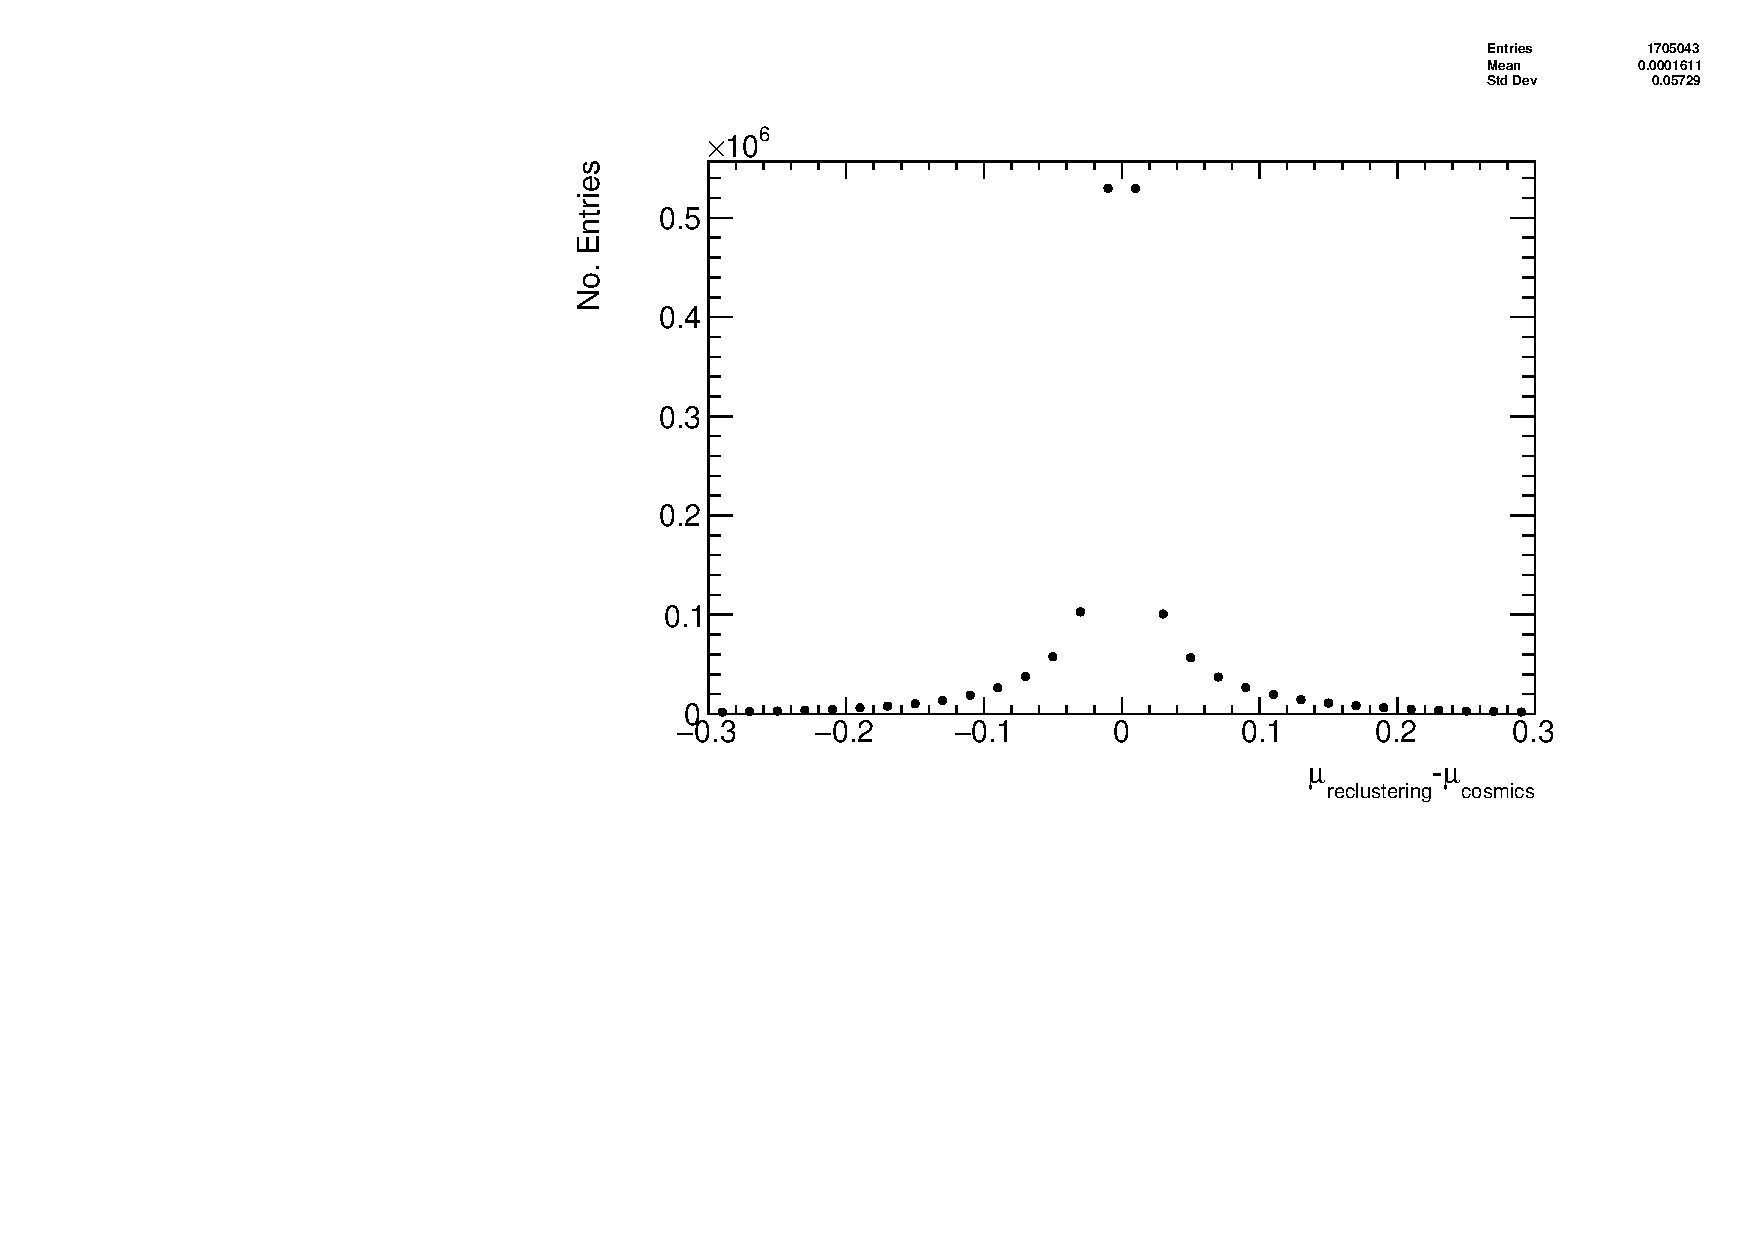
\includegraphics[width = 0.7\textwidth]{figures/figure_QL2P08_3100V_2021-05-21_reclustering_plots_mu_reclustering_minus_mu_cosmics.pdf}
    \caption{The difference between cluster means calculated with Guo's method~\cite{guo_simple_2011} in \package{tgc\_analysis/CosmicsAnalysis} and Minuit2 for ROOT~\cite{hatlo_developments_2005} in \package{strip\_position\_analysis/ReClustering} for data collected with QL2.P.8 at 3.1~kV.}
    \label{fig:mu_reclustering_minus_mu_cosmics}
\end{figure}

The RMS of the distribution in figure~\ref{fig:mu_reclustering_minus_mu_cosmics} is \SI{57}{\micro\meter}, which is much larger than the statistical uncertainty in the mean for the Minuit2 algorithm, which peaks around \SI{7}{\micro\meter}. An RMS of \SI{57}{\micro\meter} is common for data taken with most quadruplets at 3.1~kV. Therefore, the uncertainty in the y-hit positions is assigned \SI{57}{\micro\meter}.

%TODO : How does this inform the residual distribution bin size?

The x position of the cluster is taken to be the center of the wire group with the maximum detected signal, since wire groups are wide enough that usually only one wire picks up the ionization avalanche. 

%TODO : How does this inform the area of the bins we take residual means in?

%TODO : How does reclustering affect residual means?

% ==================================================
% Appendix: Analysis Statistics %
% ==================================================

\chapter[Analysis statistics]{Study of cosmics for alignment analysis statistical uncertainty}
\label{appendix:statistics}
% Edit count: 0

% Plan:
% Quantity of interest is the Gaussian mean of the residual distribution in a region of interest.
% Typically, have 1 million triggers; for QS3.P.18 got 3.5 million triggers.
% See the drop off in peak residual mean error with more triggers (FIGURE).
% We are not statistically limited. Compare residual fits for L1 F34 between 1 million triggers and 3.5 million triggers: means don't change significantly.

Typically, one million triggers (cosmic muon events, noise, photons and $\delta$-rays) were collected for each Canadian quadruplet at McGill University, resulting in roughly half the number of viable tracks after cuts. For QS3.P.18, 3.5 million triggers were collected. To gauge the sensitivity of the analysis to the available statistics, partitions of this data with each with a different number of triggers were analyzed separately. Ultimately, the quantity of interest was the Gaussian mean of the residual distribution in regions of interest, so the peak in the distribution of the statistical uncertainty in the residual means for each area of interest for a specific tracking combination was used to gauge the quality of the analysis. How the peak in the residual mean uncertainty distribution changes with the number of triggers is shown in figure for tracks on layer 1 built from layers 3 and 4 \ref{fig:res_mean_uncert_vs_triggers}. 

\begin{figure}
    \centering
    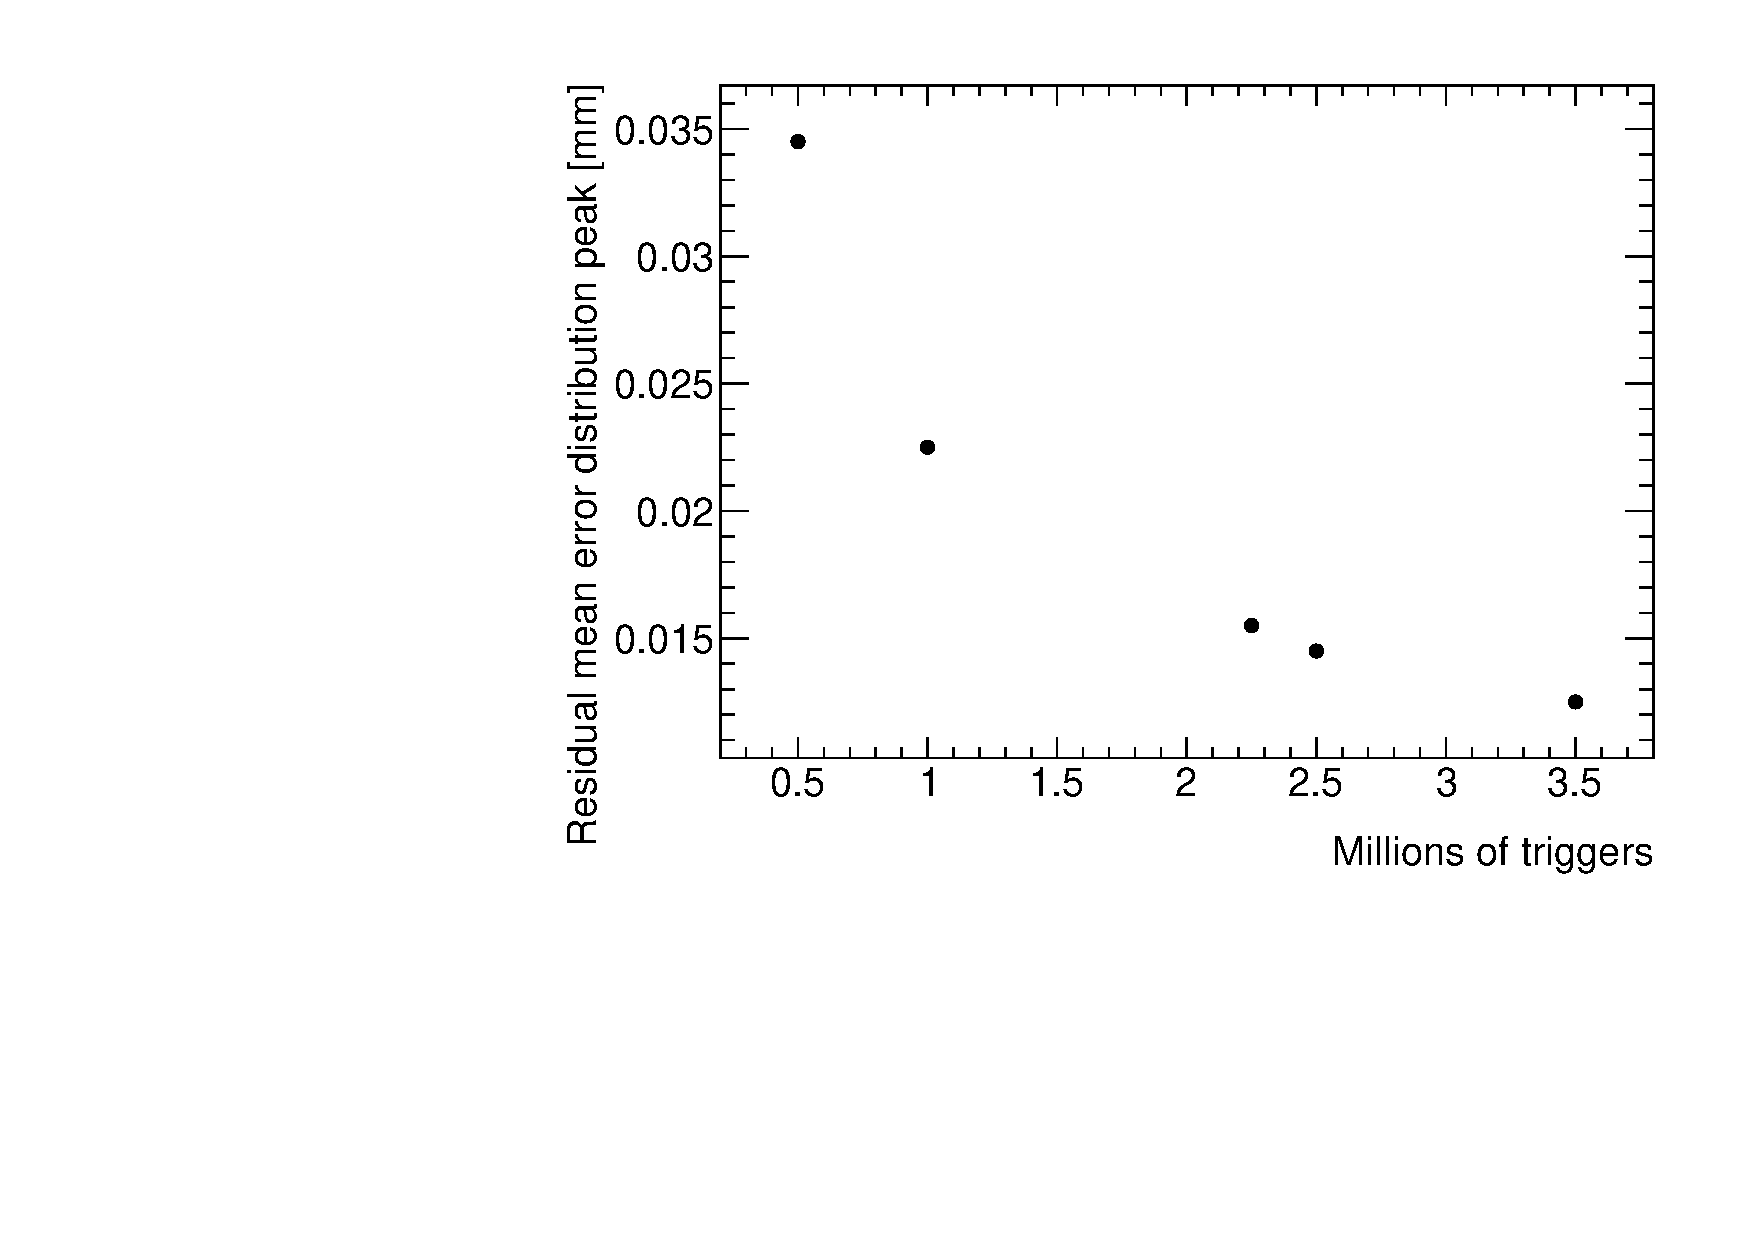
\includegraphics[width = \textwidth]{figures/figure_QS3P18_2900V_peakOfMeanErrorsDistVsTriggers_layer1_fixedlayers34.pdf}
    \caption{How the peak of the distributions of uncertainties in the residual means in regions ofinterest for tracks on layer 1 built from layers 3 and 4 changed with the number of triggers used in the analysis. The distribution falls off as $~\frac{1}{\sqrt{N}}$ as expected.}
    \label{fig:res_mean_uncert_vs_triggers}
\end{figure}

The uncertainty is already around \SI{20}{\micro\meter} at 1 million triggers, suitable for distinguishing differences in offsets of order \SI{50}{\micro\meter} as required. Although increased statistics could decrease the statistical uncertainty, it is not required for the goals of this analysis. Moreoever, the systematic uncertainty on the mean cosmics residuals is around \SI{50}{\micro\meter} so the statistical uncertainty of \SI{20}{\micro\meter} is nearly negligible.

%TODO : Include compare residual fit means for L1 F34 1 million vs 3.5 million triggers?? Do once you know how to make figures.

% ==================================================
% Appendix: Analysis Systematics %
% ==================================================

%TODO : Make mean diff plots not full page portrait. Half page would suffice. 
%TODO : Currently, section A.2 figure goes in A.3 section. Organize this once you're done writing. 
%TODO : Do I need to specify each quad? The voltage? 

\chapter[Analysis systematics]{Study of cosmics for alignment analysis systematic uncertainties}
\label{appendix:systematics}

% Sections:
% Doub gaus vs gaus -- check!
% Area bin size -- check!
% Residual distribution bin size?
%TODO 2900V vs 3100V? I think just saying strip efficiency is higher for 3100V is sufficient, although the sigmas are also smaller. But L4 F12 residual mean difference RMS is 74 um ==> Add 2900V 3100V section
% DNL
% ReClustering fit function? I think just saying I used an accepted standard is ok.

% --------------------------------------------------
\section{Residual distribution fit function}
% --------------------------------------------------
\label{appendix:systematics_res_fit_fcn}
% Edit count: 1

The distribution of residuals should be modelled by a double gaussian fit\cite{lefebvre_thesis}:

\begin{equation}
\label{eqn:doub_gaus}
G(r) = A_{s}exp\left[ \frac{-(r-\mu)^{2}}{2\sigma_s^{2}} \right] + A_{b}exp\left[ \frac{-(r-\mu)^{2}}{2\sigma_b^{2}} \right]
\end{equation}

where $r$ is the residual, $A$ is the gaussian amplitude, $\mu$ is the gaussian mean, $\sigma$ is the gaussian sigma, and the subscripts $s$ and $b$ stand for signal and background respectively. One gaussian captures the real (signal) tracks and the other captures the tracks built from noise (background). The gaussian with the smaller width is identified as the signal. 

A single gaussian fit failed less often than a double gaussian fit. The gaussian fits were performed by initially estimating the amplitude to be 100 tracks, the gaussian mean to be the histogram mean, and gaussian $\sigma$ to be the RMS. The fit range was restricted to $\pm$1 RMS from the histogram mean. The modification helped the gaussian fit capture the signal peak. An example residual distribution is shown in figure \ref{fig:double_gaussian_example_fit}. 

%TODO Why is this figure blurry?
%TODO this doesn't need to be a full page figure.

\begin{figure}
    \centering
    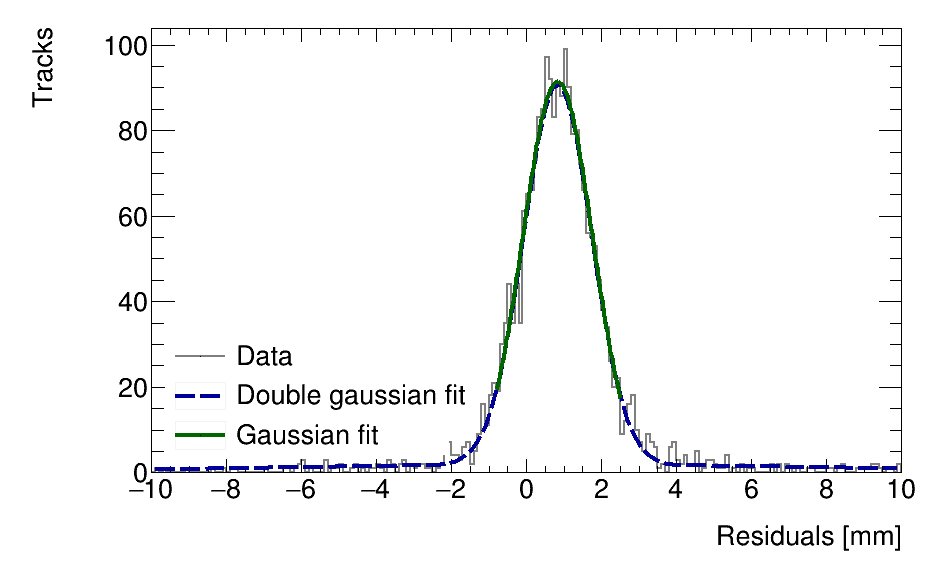
\includegraphics[width = \textwidth]{figures/figure_double_gaussian_quick_and_dirty_2900V_log_scale_gaussian_QL2C04_2900V_2021-02-08_2_xbin_10_ybin_5_100mm.png}
    \caption{Residual distribution for tracks on layer 1 built from hits on layers 3 and 4 for $x\in\left[-3.00, 97.00\right],  y\in\left[394.60, 494.60\right] mm$ for QL2.C.4 fit with a double gaussian and a single gaussian in a range of $\pm$1 RMS from the histogram mean.}
    \label{fig:double_gaussian_example_fit}
\end{figure}

For all residual distributions in \SI{100}{\milli\meter} by \SI{100}{\milli\meter} bins on layer 1 built from hits on layers 3 and 4, the difference in gaussian and double gaussian means and $\sigma$'s is shown in figure \ref{fig:double_gaussian_compare_fits}. Since the RMS of the residual mean differences distribution is less than \SI{50}{\micro\meter} the gaussian fit gave the same result within the required precision. Moreover, this is for the tracking combination with the worst extrapolation lever arm and the widest distribution of mean differences; the interpolation combinations have narrower distributions. 

The gaussian $\sigma$ should be larger than the double gaussian $\sigma$ because the gaussian distribution includes the effect of the noise tracks with large residuals, while the double gaussian models signal and background residuals separately. For this analysis, only the residual mean was important, so the systematic overestimate of the signal $\sigma$ in the gaussian fit shown on the right of figure \ref{fig:double_gaussian_compare_fits} was allowed.

\begin{figure}
    \centering
    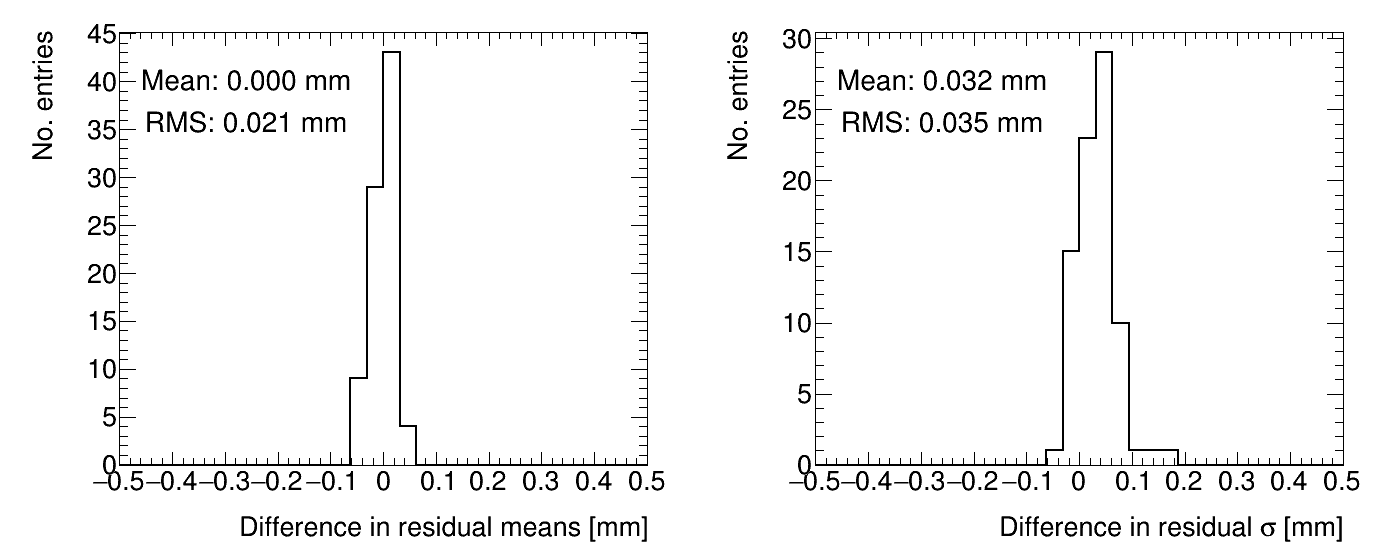
\includegraphics[width = \textwidth]{figures/figure_compare_residual_fits_QL2C04_2900V_2021-02-08_2_fit_range_mean_pm_RMS_minus_quick_and_dirty_2900V_log_scale_layer1_fixedlayers34.png}
    \caption{Difference in residual distribution means and $\sigma$'s for a gaussian and double gaussian fit, for all residual distributions in \SI{100}{\milli\meter} by \SI{100}{\milli\meter} bins on layer 1 built from hits on layers 3 and 4 for QL2.C.4, data taken at 2900 V.}
    \label{fig:double_gaussian_compare_fits}
\end{figure}

% --------------------------------------------------
\section{Area of residual distribution regions of interest}
% --------------------------------------------------
\label{appendix:systematics_bin_size}
% Edit count: 1
% DO I NEED TO EXPLAIN THIS IN MATH? I tried on June 3rd in my notes, it's complicated for such a simple thing.
% If this flies, you'll need to establish that reference frame == two fixed layers' frame as jargon in your thesis.
% Also need to establish x == perpendicular to wires; y == perpendicular to strips. ==> How do I do this consistently?
% May need to add 3100V reference if it's not already defined in your thesis.
% Define ROI as short form?

%TODO : How do I cite the distribution of rotations angles by Dylan?
The area of the region of interest in which to include tracks is primarily motivated by the misalignment model: the width of the region should be less than the scale on which the local offset is expected to change significantly. Changes in offset of order \SI{50}{\micro\meter}, the approximate position resolution of the sTGCs in the $\eta$-coordinate, are significant. In a misalignment model with an offset and rotation, only the rotation changes the local offset with respect to the x-coordinate \footnote{The effect of rotation can be modeled by assuming the recorded track position is related to the hit position by a passive rotation. The angle of rotation is the relative angle between the layer of interest and the nominal geometry. The local offset does change with respect to the track's y coordinate as well, but negligibly in the limit of small rotation angles.}.  The distribution of the as-built cathode board rotation angles shows that the RMS of the rotation angle is \SI{200}{\micro\radian} [https://indico.cern.ch/event/1035057/ PG. 18]; however, the distribution has a long tail so a typical rotation angle of \SI{1000}{\micro\radian} was used here. A rotation of \SI{1000}{\micro\radian} will cause a \SI{50}{\micro\meter} change in local offset over a change in x of \SI{50}{\centi\meter}. Therefore, the width of the region of interest should be less than \SI{500}{\milli\meter}.

Two other factors inform the width of the region. First, since the hits' x-coordinates are discrete the width in x must be larger than the pitch of the wire groups to ensure the bin will have a sufficient number of tracks fall in it. Second, more tracks will be included in a larger area so more statistics will be available for the residual distribution fit. For the bin widths wider than two wire groups, the statistics are sufficient. For each x-ray residual, the mean cosmics residual was calculated for a few different bin widths, and the difference in means plotted. Figure \ref{fig:area_bin_size_mean_diff} shows an example for QL2.C.4. The width of the distribution is on the order of \SI{50}{\micro\meter}, showing that the calculation of the residual mean is relatively robust with respect to the area of the bin. However, \SI{50}{\micro\meter} is greater than the typical statistical uncertainty on the cosmic residual of means, which ranges from \SI{10}{\micro\meter} - \SI{40}{\micro\meter} depending on the tracking combination under study. Therefore, the cosmic residual means are assigned an uncertainty of \SI{50}{\micro\meter}.
%TODO : Verity that you actually apply the 50 um uncertainty.

%TODO : This figure should have the mean and rms on it.
\begin{figure}
    \centering
    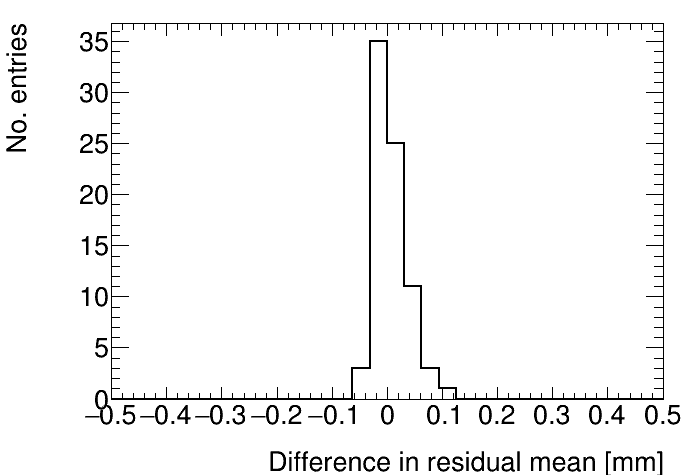
\includegraphics[width = \textwidth]{figures/compare_residual_fits_around_xrays_QL2C04_3100V_2021-05-20_100mm_width_bins_minus_QL2C04_3100V_2021-06-02_200mm_width_bins_means_difference.png}
    \caption{Difference in cosmic residual means around x-ray residuals for square bins of 100 mm width and 200 mm width for QL2.C.4.}
    \label{fig:area_bin_size_mean_diff}
\end{figure}

For this analysis, \SI{100}{\milli\meter} by \SI{100}{\milli\meter} by \SI{100}{\milli\meter} bins were used.

% --------------------------------------------------
\section{Differential non-linearity}
% --------------------------------------------------
\label{appendix:systematics_dnl}
% Edit count: 1
In this context, differential non-linearity (DNL) is when the reconstructed cluster mean is biased by the fit of the discretely sampled PDO distribution over the strips. The bias depends on the relative position of the avalanche with respect to the center of the closest strip. For a summary of DNL, refer to page 40 of Lefebvre's thesis \cite{lefebvre_thesis}. The cluster mean was corrected for DNL using the equation:
\begin{equation}
\label{eqn:dnl_corr}
y' = y + a \sin \left( 2 \pi y_{rel} \right)
\end{equation}

where $y$ is the cluster mean, $y_{rel}$ is the relative position of the cluster mean with respect to the strip's center, $a$ is the amplitude of the correction, and $y'$ is the corrected cluster mean. The amplitude can be derived by comparing the reconstructed hit position to the expected hit position, as done in Abusleme, 2016 \cite{abusleme_performance_2016}. With cosmic muons, there is no reference hit position to compare to, so track residuals were used as a proxy \cite{lefebvre_thesis}. The hallmark of the DNL effect is the periodic pattern in the residual versus $y_{rel}$ profile, and the effect of correcting the cluster means using an amplitude of \SI{50}{\micro\meter} is shown in figure \ref{fig:dnl_corr_effect}. An amplitude of \SI{50}{\micro\meter} was based on Lefebvre's estimate of the DNL amplitudes by layer, quadruplet and cluster size using exclusive cosmic muon tracks in \package{tgc\_analysis/CosmicsAnalysis}. Little variation was seen in the amplitude parameters with respect to the quadruplet tested, the layer and the cluster size so a universal correction was used.
%TODO How little is little? Check your notes.
%TODO exclusive better be defined somewhere clearly.

\begin{figure}
    \centering
    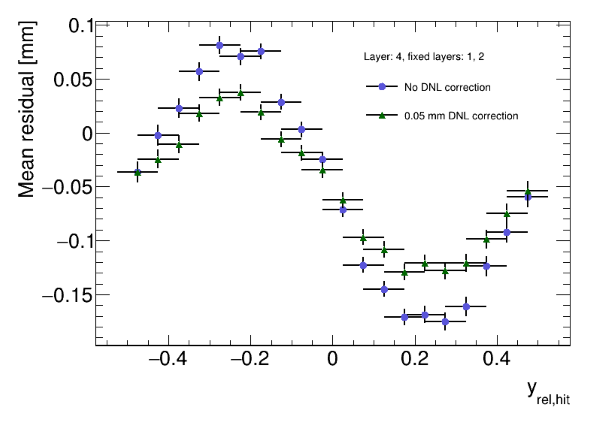
\includegraphics[width = \textwidth]{figures/figure_dnl_profiles_blue_QL2P08_3100V_2021-06-18_no_dnl_green_QL2P08_3100V_2021-06-18_2_50um_universal_DNL_layer4_fixed12.png}
    \caption{Effect applying a \SI{50}{\micro\meter} DNL correction to the cluster means on the residual vs $y_{rel}$ distribution for tracks built from layers 1 and 2 and extrapolated to layer 4 for QL2.P.8.}
    \label{fig:dnl_corr_effect}
\end{figure} 

Although the correction is not large enough in this case, the figure shows that the correction does reduce the DNL effect. Slightly better performance is seen in the interpolation tracking combinations where the quality of the residuals is better. DNL corrections for cosmic muon data are difficult because the DNL effect is obscured by the effect of misalignments and noise. Misalignments cause the center of the sine pattern in figure \ref{fig:dnl_corr_effect} to be shifted off of zero, since the mean of residuals is shifted.

In figure \ref{fig:dnl_compare_fits}, it is apparent that the effect of the DNL correction on the mean of the residual distribution in \SI{100}{\milli\meter} by \SI{100}{\milli\meter} areas is on the order of micrometers in the worst extrapolation case. Although the $\sigma$'s of the residual distributions shrink with the DNL correction, the mean is the parameter of interest. Therefore, for this analysis DNL was not corrected for.

\begin{figure}
    \centering
    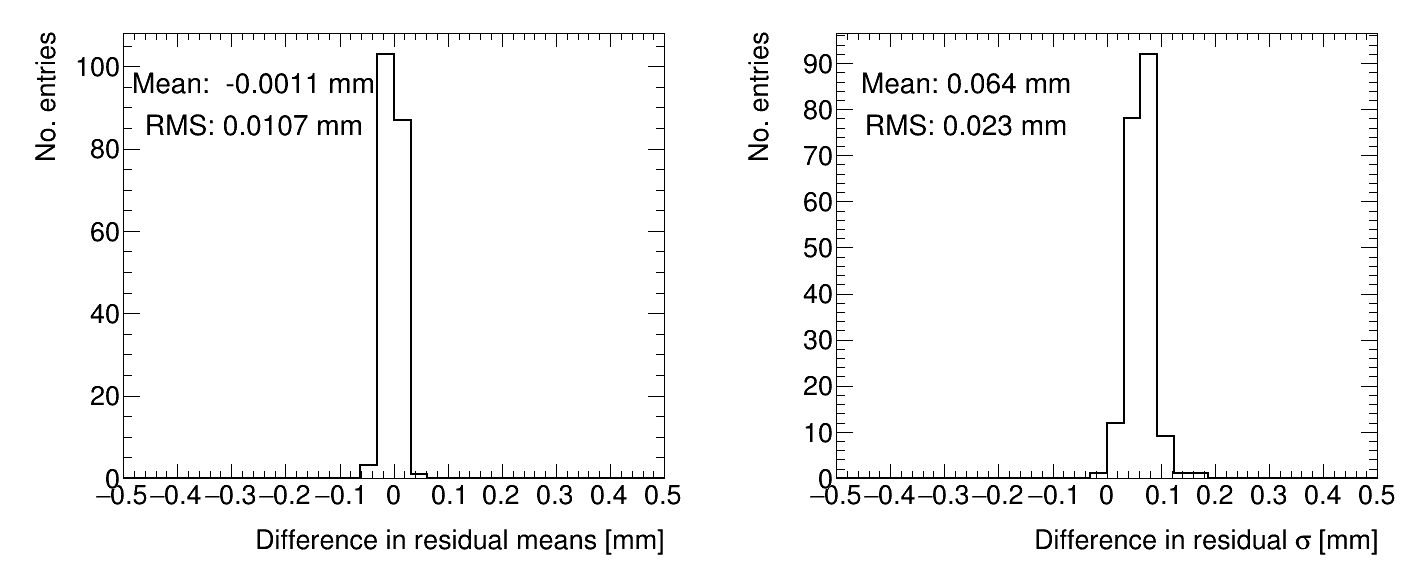
\includegraphics[width = \textwidth]{figures/figure_compare_residual_fits_QL2P08_3100V_2021-06-18_no_dnl_minus_QL2P08_3100V_2021-06-18_2_50um_universal_DNL_layer4_fixedlayers12.png}
    \caption{Difference in residual distribution means and $\sigma$'s with and without DNL correction for residuals on layer 4 from reference layers 1 and 2 for QL2.P.8.}
    \label{fig:dnl_compare_fits}
\end{figure}
































% ==================================================
% Appendix: Printable plots %
% ==================================================

\chapter[Printable plots]{Printable plots}
\label{appendix:print}
% Edit count: 0

\begin{figure}
    \centering
    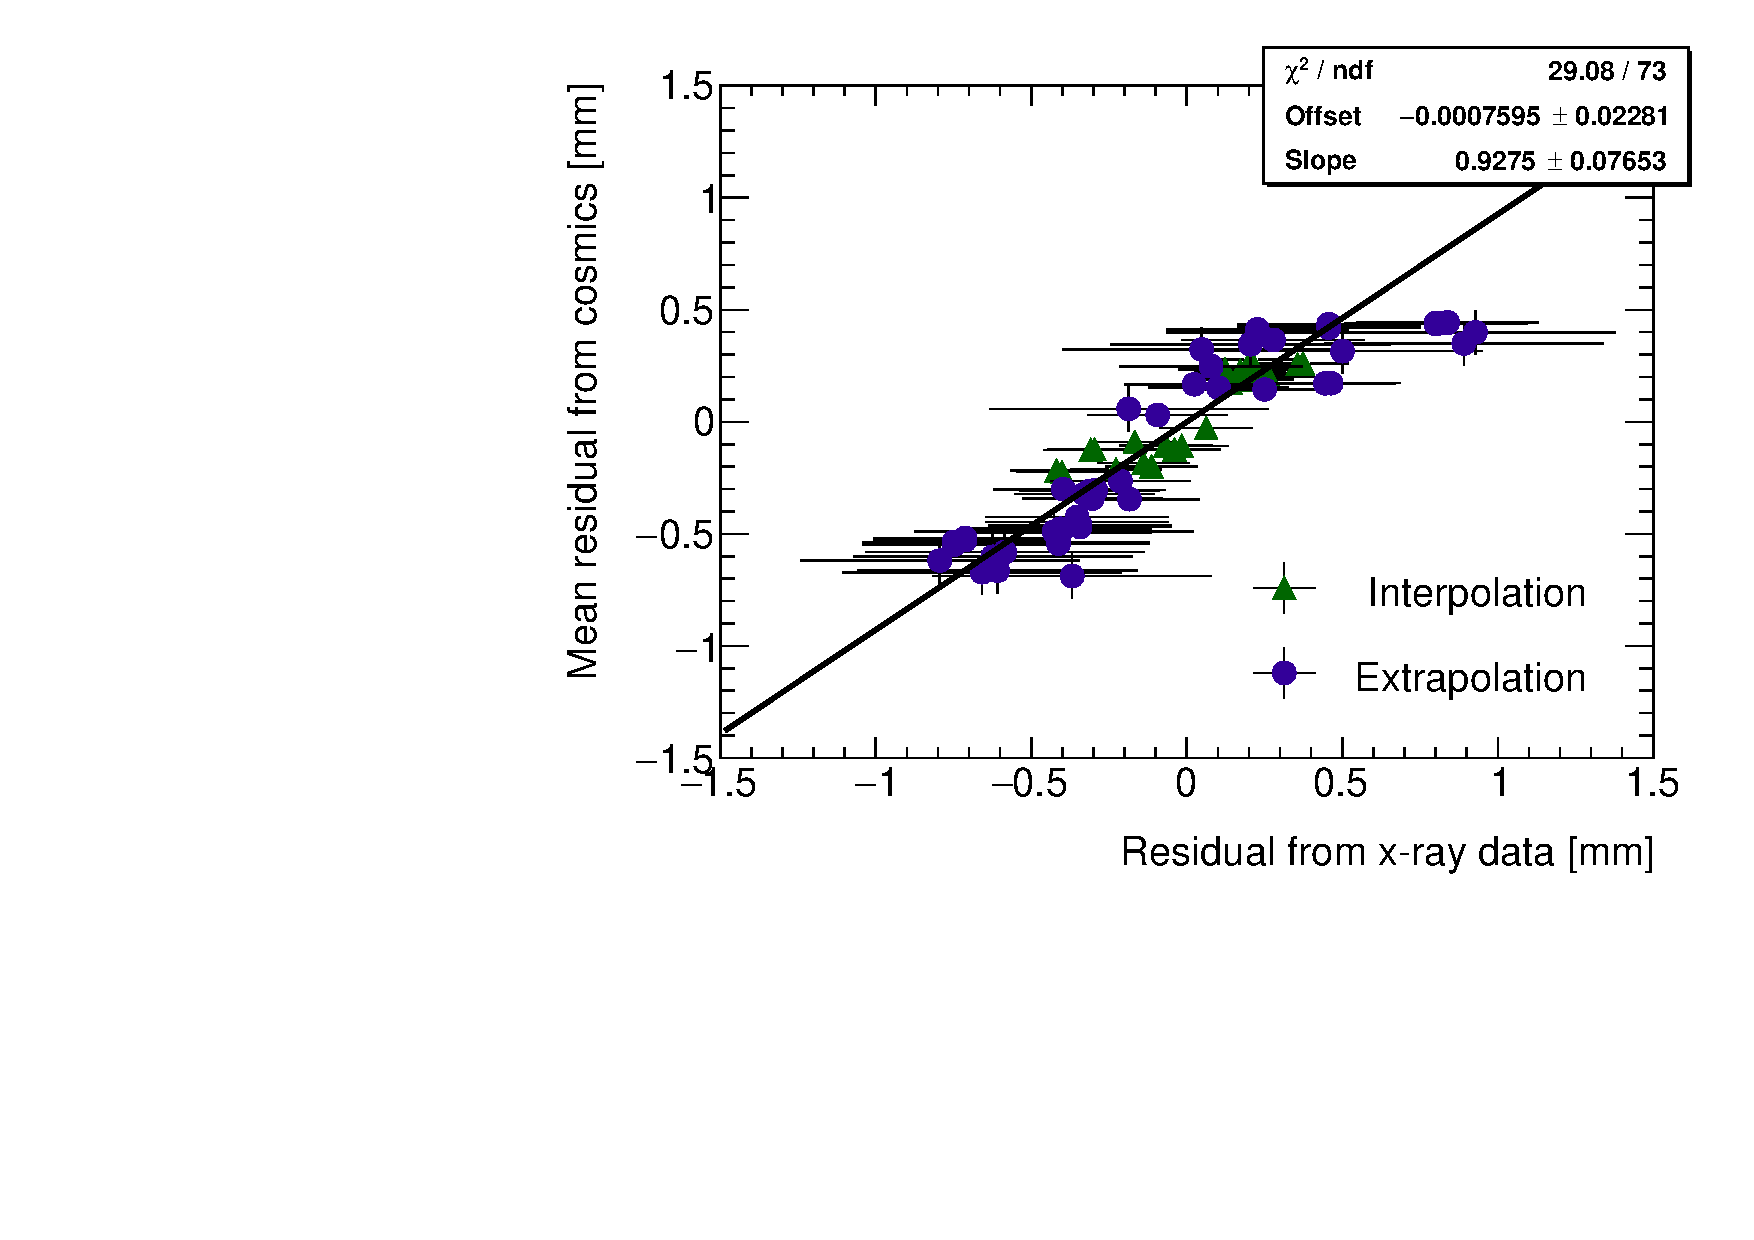
\includegraphics[width = \textwidth]{figures/figure_QL2P11_3100V_2021-08-05_QL2P11_local_cosmic_and_xray_data_correlation_plot_printable.pdf}
    \caption{Correlation plot between x-ray and cosmics residuals for all tracking combinations for QL2.P.11. Each rectangle is centered on an x-ray and mean cosmics residual pair. The width of the rectangles in $x$ and $y$ are the uncertainty in the x-ray and mean cosmics residual respectively. A printable version of figure~\ref{fig:correlation} in section~\ref{sec:assessing_correlation}.}
    \label{fig:correlation_print}
\end{figure}

\begin{figure}
    \centering
    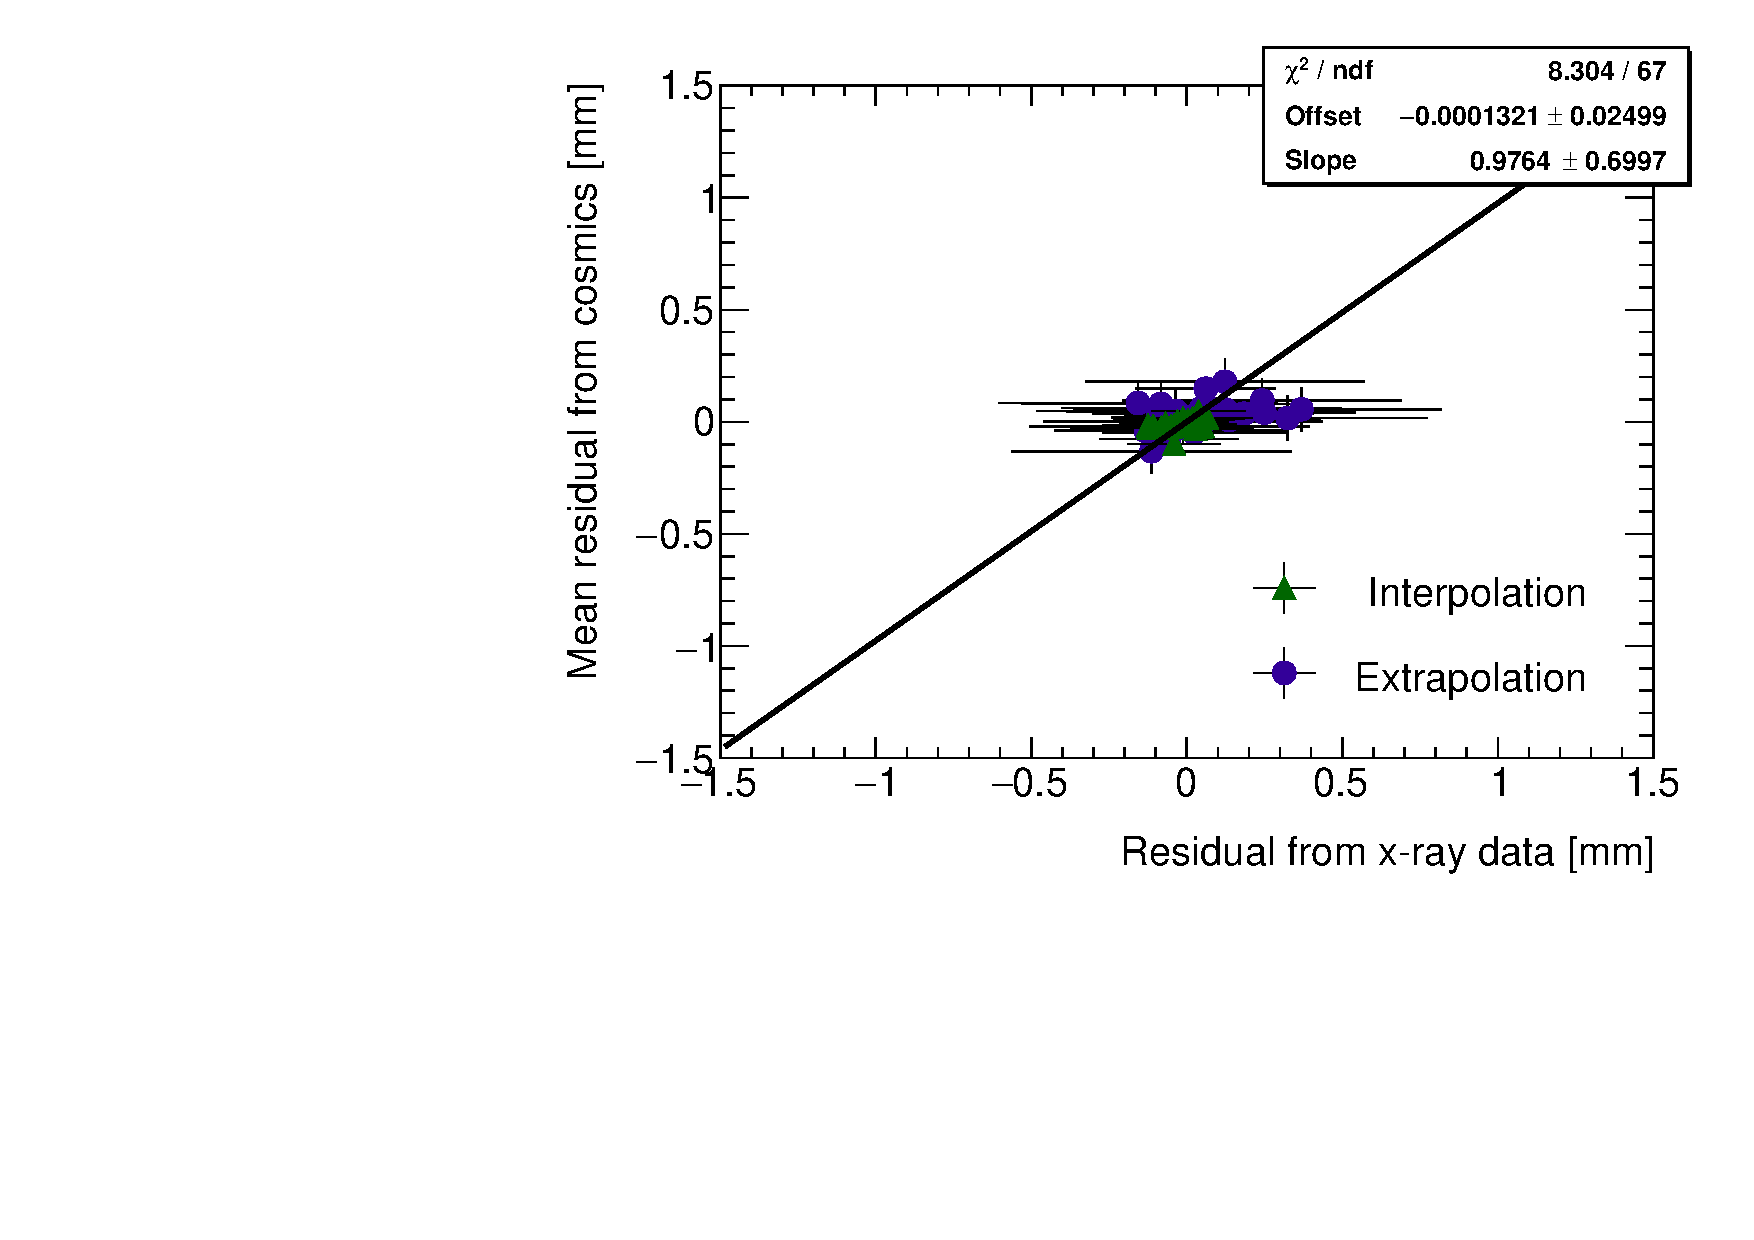
\includegraphics[width = \textwidth]{figures/figure_QL2P08_3100V_2021-08-16_QL2P08_local_cosmic_and_xray_data_correlation_plot_printable.pdf}
    \caption{Correlation plot between x-ray and cosmics residuals for all tracking combinations for QL2.P.8. Each rectangle is centered on an x-ray and mean cosmics residual pair. The width of the rectangles in $x$ and $y$ are the uncertainty in the x-ray and mean cosmics residual respectively. A printer friendly version of this plot is available. A printable version of figure~\ref{fig:no_correlation} in section~\ref{sec:assessing_correlation}.}
    \label{fig:no_correlation_print}
\end{figure}

% GLOSSARIES (Lists of definitions, abbreviations, symbols, etc. provided by the glossaries-extra package)
% -----------------------------
% \printglossaries
% \cleardoublepage
% \phantomsection		% allows hyperref to link to the correct page

%----------------------------------------------------------------------
\end{document} % end of logical document
